%                                     MMMMMMMMM
%
%  MMA    MM   MMMMMM  MMMMMMM   MM    MMMMMMMM   MMA   MM  MMMMMMM MMMMMMM
%  MMMA AMMM   MM        MM     MMMM              MMMM  MM  MM        MM
%  MM MMM MM   MMMMMM    MM    IM  MI   MMMMMMM   MM MMxMM  MMMMMM    MM
%  MM  M  MM   MM        MM   .MMMMMM.            MM  MMMM  MM        MM
%  MM     MM   MMMMMM    MM   MM    MM            MM   MMM  MMMMMMM   MM
%
%
%          - META-NET Strategic Research Agenda | English SRA -
% 
% ----------------------------------------------------------------------------

\documentclass[10pt, plain]{../../metanetpaper}

\usepackage{acronym}

%!TEX TS-program = xelatex
\RequireXeTeX %Force XeTeX check

%                                     MMMMMMMMM
%
%  MMA    MM   MMMMMM  MMMMMMM   MM    MMMMMMMM   MMA   MM  MMMMMMM MMMMMMM
%  MMMA AMMM   MM        MM     MMMM              MMMM  MM  MM        MM
%  MM MMM MM   MMMMMM    MM    IM  MI   MMMMMMM   MM MMxMM  MMMMMM    MM
%  MM  M  MM   MM        MM   .MMMMMM.            MM  MMMM  MM        MM
%  MM     MM   MMMMMM    MM   MM    MM            MM   MMM  MMMMMMM   MM
%
%
%          - META-NET Strategic Research Agenda | English Metadata -
% 
% ----------------------------------------------------------------------------

\usepackage{polyglossia}
\setotherlanguages{english}

\title{Strategic Research Agenda for Multilingual Europe 2020 --- ~}

\spineTitle{The META-NET Strategic Research Agenda for Multilingual Europe 2020}

\subtitle{~ --- ~}

\author{
  Aljoscha Burchardt \\
  Georg Rehm \\
  Hans Uszkoreit \\
  \footnotesize{(editors)}
}

\authoraffiliation{
  Aljoscha Burchardt~ {\small DFKI}\\
  Georg Rehm~ {\small DFKI}\\
  Hans Uszkoreit~ {\small DFKI, Universität des Saarlandes}\\
  \footnotesize{(editors)}
}

\editors{
  % Georg Rehm, Hans Uszkoreit\\(editors)
}

% Text in left column on backside of the cover
\SpineLText{%
}

% Text in right column on backside of the cover
\SpineRText{%
}

% Quotes from VIPs on backside of the cover
\quotes{% 
  In everyday communication, Europe’s citizens, business
  partners and politicians are inevitably confronted with language
  barriers. Language technology has the potential to overcome these
  barriers and to provide innovative interfaces to technologies and
  knowledge. This document presents a Strategic Research Agenda for
  Multilingual Europe 2020.
  %
  The paper was prepared by META-NET, a Network of Excellence
  funded by the European Commission. META-NET consists of 60 research
  centres in 34 countries, who cooperate with stakeholders from
  economy, government agencies, research organisations,
  non-governmental organisations, language communities and European
  universities. META-NET’s vision is high-quality language technology
  for all European languages.\\\\
  %
  ``The research carried out in the area of language technology is of
  utmost importance for the consolidation of Portuguese as a language
  of global communication in the information society.''\\
  \textcolor{grey2}{--- Dr.~Pedro Passos Coelho (Prime-Minister of
  Portugal)}\\[2mm]
  %
  ``It is imperative that language technologies for Slovene are
  developed systematically if we want Slovene to flourish also in the
  future digital world.''\\
  \textcolor{grey2}{--- Dr. Danilo Türk (President of the Republic of
  Slovenia)}\\[2mm]
  %
  ``For such small languages like Latvian keeping up with the ever
  increasing pace of time and technological development is
  crucial. The only way to ensure future existence of our language is
  to provide its users with equal opportunities as the users of larger
  languages enjoy. Therefore being on the forefront of modern
  technologies is our opportunity.''\\ \textcolor{grey2}{--- Valdis
  Dombrovskis (Prime Minister of Latvia)}\\[2mm]
  %
  ``Europe's inherent multilingualism and our scientific expertise are
  the perfect prerequisites for significantly advancing the challenge
  that language technology poses. META-NET opens up new opportunities
  for the development of ubiquitous multilingual technologies.''\\
  \textcolor{grey2}{--- Prof. Dr. Annette Schavan (German Minister of
  Education and Research)} }

% Funding notice
\FundingNotice{%
  The development of the META-NET Strategic Research Agenda for
  Multilingual Europe 2020 has been funded by the Seventh Framework
  Programme of the European Commission under the contract T4ME (Grant
  Agreement 249\,119).}

% LTInfoBox
\LTInfoBox{
  \begin{tabular}{p{.90\linewidth}}
  \rowcolor{orange2}\vspace{.10cm}\centerline{{\textcolor{white}{\Large  What is Language Technology?}}}\\[-2mm]
  \rowcolor{orange2} Language technologies are specialised information technologies for processing automatically the most complex information medium in our world: \emph{human languages} -- in both modalities (spoken and written language) and also in both directions (analysis and generation of language). 

  Language technologies are developed by experts involved in computer
  science, linguistics, computational linguistics and related
  disciplines. References: \cite{jurafsky-martin01,manning-schuetze1,lt-world1,lt-survey1}
  \vspace*{3mm} \\

  \rowcolor{orange1} \vspace{.15cm}\centerline{{\textcolor{white}{\Large  What are common Language Technology applications?}}}\\[-2mm]
  \rowcolor{orange1} Spell and grammar checking in text processing applications and editing tools; 
  web search; voice dialing; interactive dialogue systems (from banking over the phone to train reservation systems to Apple's Siri); cross-lingual search in digital libraries (such as, e.\,g., Europeana); synthethic voices for navigation systems; recommender systems for online shops; machine translation systems such as Google Translate, etc.
  \vspace*{3mm} \\ 

  \rowcolor{orange2} \vspace{.15cm}\centerline{{\textcolor{white}{\Large  What are the major topics?}}}
  \center
  \begin{tabular}{p{.30\linewidth} p{.30\linewidth}p{.30\linewidth}}
  \rowcolor{yellow} \vspace{.001cm} {\Large Information} & \vspace{.001cm} {\Large Communication} & \vspace{.001cm}  {\Large Translation} \\[-1.2mm]
  \rowcolor{yellow} \small Access and management & \small Human-human; human-machine & \small Spoken and written \\[.4em]
  \rowcolor{yellow} Example: & Example: & Example: \\[-1.2mm]
  \rowcolor{yellow} Information retrieval & Spoken dialogue system & Document translation\\[2mm]
  \end{tabular}
  \vspace*{2mm} \\

  \end{tabular}
}


\begin{document}

\maketitle

\cleardoublepage

\pagenumbering{roman}
\makefundingnotice

\cleardoublepage

% ----------------------------------------------------------------------------

\ssection*[What Europe says]{What Europe says}

\textbf{Croatia:} ``Language technologies play [\dots] a crucial role in showcasing the linguistic richness of Europe [\dots].'' --- Prof.~Milena Žic Fuchs (Fellow of the Croatian Academy of Sciences and Arts, Chair of the Standing Committee for the Humanities of the European Science Foundation)

\medskip \textbf{Czech Republic:} ``META-NET brings a significant contribution to the technological support for languages of Europe and as such will play an indispensable role in the development of multilingual European culture and society.'' --- Prof.~Ing.~Ivan Wilhelm, CSc., Dr.~h.\,c.~mult.~(Deputy minister for education, youth and sport)

\medskip \textbf{Denmark:} ``If we have the ambition to use the Danish language in the technological universe of the future, an effort must be made now to maintain and further develop the knowledge and expertise that we already have. This emerges from the META-NET report with great clarity. Otherwise we run the risk that only people who are fluent in English, will profit from the new generations of web, mobile and robot technology which are up and coming.'' --- Dr.~Sabine Kirchmeier-Andersen (Director of the Danish Language Council)

\medskip ``Given the right attention, the diversity of the European languages can enrich the cultural and commercial development in Europe.  However, if not properly addressed the linguistic diversity can be a serious threat to Europe’s global economic growth. The META-NET [SRA] makes way for essential discussions and initiatives, may it be read by many!'' --- Bo Vincents (CEO, Ankiro)

% \medskip ``A focus on language technology is one of the most important tools for preserving the linguistic diversity that is one of the core values of the EU. This is why META-NET is so important. After all, multilingualism in Europe contributes to exactly what the EU wishes to stand for: Democracy, equality and transparency. The increased focus on the development of language technology underpins these core values in a digital age. Communication between businesses, between organisations, and within the public sector across borders is highly dependent on language technology. There is also an indisputable democratic aspect to language technology in that it offers all inhabitants in the EU the opportunity to contribute economically, politically and socially to the European project, which affects all of our lives. Language technology will be essential to breaking down the linguistic and cultural barriers which are otherwise bound to develop.'' --- Sanne Hoffensetz Andresen (Ordbogen)

\medskip \textbf{Estonia:} ``If we do not implement the development plan for language technology or do not cooperate with other countries in the same direction, in future Estonian will [\dots] be marginalized in information society.'' --- Development Plan of the Estonian Language 2011--2017

\medskip \textbf{Finland:} ``Without languages we could not communicate. The META-NET network is a valuable support for a multilingual Europe.'' --- Alexander Stubb (Minister for European Affairs and Foreign Trade of Finland)

\medskip ``The big issues are handled well. This is a good agenda!'' --- Niko Papula (Managing Director, Multilizer)

\medskip \textbf{France:} ``META-NET provides an invaluable contribution to the development of a genuine European strategy in support to multilingualism, based on existing technologies while encouraging the development of new innovative technologies.'' --- Xavier North (Délégué Général à la Langue Française et aux Langues de France)

% \medskip ``The SRA is a very important document!'' --- Max Silberztein (Université de Franche-Comté)

% \medskip ``I am very happy to have been able to read the [\dots] SRA.'' --- Antonio Balvet (Université Lille~3)

\medskip \textbf{Germany:} ``Europe's multilingualism and our scientific expertise are the perfect prerequisites for significantly advancing the challenge that language technology poses. META-NET opens up new opportunities for the development of ubiquitous multilingual technologies.'' --- Prof.~Dr.~Annette Schavan (German Minister of Education and Research)

% \medskip ``Thanks to all of you for putting together such an impressive document!'' --- Miriam Butt (University of Konstanz)

% \medskip ``The [SRA] represents myself and also my area of research very well. I would like to thank you for all the hard work and effort you put into this!'' --- David Schlangen (University of Bielefeld)

% \medskip ``Thank you for the excellent SRA.'' --- Günther Roscher (ICS Dr.~G.~Roscher GmbH)

% \medskip ``META-NET have laid out a highly compelling vision of how Europe can bridge the digital and the analog, the computer and the human, thus strengthening the communication between us humans -- while preserving our cultural diversity. And not only do they have the vision; their SRA shows that clearly do they have the means, too. For us as a company building social media research tools for the knowledge workers of tomorrow, their research themes are bound to feed right into the success of our core products.'' --- Matthias Bärwolff (Tazaldoo)

% \medskip ``The SRA is a really good piece of work.'' --- Caterina Berbenni-Rehm (FUTUREtec)

\medskip ``Global communications are a significant success factor for a globally active company. Accordingly, their importance is steadily increasing with the increased globalization and growing complexity of international business. In this context, the design of effective and efficient language management processes makes an important contribution. The development of language technologies already plays a decisive role today and will continue to do so in the future. META-NET makes a pivotal contribution in the area of reseach and maintenance of networks with developers and users of language technologies.'' ---
Johannes Bursch (Head of Corporate Language Management, Daimler AG)

\medskip \textbf{Greece:} ``Further support to language technologies safeguards the presence of Greek language and culture in the digital environment, while at the same time promoting development and fostering communication among citizens within the Information Society.'' --- George Babiniotis (Minister of Education, Lifelong Learning and Religious Affairs)

\medskip \textbf{Hungary:} ``META-NET is making a significant contribution to innovation, research and development in Europe and to an effective implementation of the European idea.'' --- Valéria Csépe (Deputy General Secretary of Hungarian Academy of Sciences)

\medskip ``I am happy that such a paper and a common effort for research is planned in such a way and I [am] excited about this common effort.'' --- Attila Törcsvári (Arcanum Development)

\medskip \textbf{Iceland:} ``Language technology is an essential tool in a variety of linguistic research, and supports the official Icelandic policy of promoting the national language in all aspects of communication.'' --- Dr.~Guðrún Kvaran (Chair of the Icelandic Language Council)

\medskip \textbf{Ireland:} ``Language technology is no longer a luxury for most European languages -- it is now essential to their survival as viable means of expression across the whole range of areas from business to the arts, and this is as much the case for Irish as any other European language.'' --- Ferdie Mac an Fhailigh (CEO, Foras na Gaeilge)

\medskip \textbf{Israel:} ``Congratulations on the [\dots] SRA. This is an impressive document.'' --- Ilan Kernerman (CEO, K Dictionaries)

\medskip \textbf{Latvia:} ``For such small languages like Latvian keeping up with the ever increasing pace of time and technological development is crucial. The only way to ensure future existence of our language is to provide its users with equal opportunities as the users of larger languages enjoy. Therefore being on the forefront of modern technologies is our opportunity.'' --- Valdis Dombrovskis (Prime Minister of Latvia)

\medskip \textbf{Lithuania:} ``Conserving [Lithuanian] for future generations is a responsibility of the whole of the European Union. How we proceed with developing information technology will pretty much determine the future of the Lithuanian language.'' --- Andrius Kubilius (Prime Minister of the Republic of Lithuania)

% \medskip \textbf{Luxembourg:} ``This is a European challenge of enormous importance!'' --- Roman Jansen-Winkeln (CTO, Belingoo Media Group)

\medskip \textbf{Malta:} ``It will be really unfortunate if we do not exploit the developments in technology to apply them to the linguistic field. The synergy between these two sciences has to be brought to the service of the people so that it makes our life easier and helps to break the barriers in a globalised world. Thus the technology support for the Maltese language should serve our language to be continuously cultivated, used and placed on the same level as other languages.'' --- Dolores Cristina (Minister for Education and Employment)

\medskip ``The SRA is very stimulating, exhaustive and effective.'' --- Ray Fabri (National Council for the Maltese Language)

\medskip \textbf{Netherlands:} ``I like the vision described very much and the research priorities formulated.'' --- Alice Dijkstra (Nederlandse Organisatie voor Wetenschappelijk Onderzoek)

\medskip ``The SRA provides an interesting and stimulating outlook for the years ahead in a quickly evolving landscape.'' --- Marc Kemps-Snijders (Meertens Instituut)

\medskip \textbf{Poland:} ``Language technologies [\dots] will have a growing influence on capabilities and communication models of the contemporary world as well as on the way human natural languages, such as the Polish language, take part in this process. [Language technologies] are more and more present in our everyday life. For their presence to be rational and functional, for it to serve the needs of the economy, as well as the social and cultural life well, further large-scale work in this area is needed.'' --- Prof.~Michał Kleiber (President of the Polish Academy of Sciences)

\medskip \textbf{Portugal:} ``The research carried out in the area of language technology is of utmost importance for the consolidation of Portuguese as a language of global communication in the information society.'' --- Dr.~Pedro Passos Coelho (Prime-Minister of Portugal)

\medskip \textbf{Romania:} ``We write messages on the mobile phone and we are not even aware of the technology that predicts the words we intend to write. Linguistic technologies represent a central element of the European Union, because languages themselves occupy a central place in the functioning of the EU.'' --- Leonard Orban (former European Commissioner for Multilingualism)

\medskip \textbf{Slovenia:} ``It is imperative that language technologies for Slovene are developed systematically if we want Slovene to flourish also in the future digital world.'' --- Dr.~Danilo Türk (President of the Republic of Slovenia)

\medskip \textbf{Spain:} ``I like the spirit of the agenda!'' --- Juanjo Bermudez (Founder, Lingua e-Solutions SL)

\medskip \textbf{Sweden:} ``High-quality language technology may be the most effective means of preserving the linguistic diversity of Europe. Being able to use all languages fully in modern society is a question of democracy. In this connection META-NET fulfils a central, even crucial, function.'' --- Lena Ekberg (Swedish Language Council)

% \medskip ``A joint Nordic challenge is the development of language technology for texting and reading subtitles. The Nordic countries are small language areas, and therefore the market is not driving the development of language technology by itself. However, the need for reading subtitles is large, because we in the Nordic countries have a tradition of subtitling foreign broadcasts instead of dubbing them, as in many other countries.'' --- Rickard Domeij (head of the Swedish Language Council)

\medskip ``Thank you for authoring this text! [The SRA] will provide great support for many interesting and necessary research and development projects in the near future!'' --- Jussi Karlgren (CEO, Gavagai)

% \medskip ``The Priority Research Themes hit the bull's eye. Let's all hope for the best for the report.'' --- Jens Erik Rasmussen (New Business Manager, Mikro Værkstedet)

% \medskip ``Thank you for the work that went into compiling the SRA. It is impressive and clearly shows coverage of the LT area hot topics.'' --- Olga Caprotti (University of Gothenburg)

\medskip \textbf{Turkey:} ``This agenda is excellent.'' --- Erhan Mengusoglu (Mantis Software)

\medskip \textbf{UK:} ``Language is a fundamental part of society. Research into Language Technology has already led to the development of software that many people are familiar with, when searching the web, checking spelling in a word processor or booking cinema tickets over the telephone. The work of META-NET is an important step towards a future in which Language Technology will be all around us, allowing us to collaborate, conduct business and share knowledge with friends and colleagues, whether or not we speak the same language.'' --- David Willets (Minister of State for Universities and Science, Department for Business, Innovation and Skills)

\medskip \textbf{European Commission:} ``Having worked on automatic media analysis for many years and in tens of languages, we are painfully aware of the lack of text analysis tools and resources in most languages. META-NET's analysis is very accurate. Language Technology is a key enabling ingredient for future generations of IT. Languages for which no tools and resources will exist soon will not participate in the next major technological developments.'' --- Ralf Steinberger (Joint Research Centre, 
IPSC -- GlobeSec -- Open-Source Text Information Mining and Analysis, Ispra, Italy)

\smallskip \centerline{\small See \url{http://www.meta-net.eu/whitepapers/all-quotes-and-testimonials} for additional quotes and testimonials.}

\clearpage

~

\vfill

\centerline{\normalsize\fbox{\parbox{\dimexpr 0.85\linewidth - 2\fboxrule - 2\fboxsep}{``The Commission will [\dots] work with stakeholders to develop a new generation of web-based applications and services, including for multilingual content and services, by supporting standards and open platforms through EU-funded programmes.'' -- \emph{A Digital Agenda for Europe} \cite{DA2010}, p.~24}}}

\bigskip
\centerline{\normalsize\fbox{\parbox{\dimexpr 0.85\linewidth - 2\fboxrule - 2\fboxsep}{``Everybody must have the chance to communicate efficiently in the enlarged EU. This does not only affect those who already are multilingual but also those who are monolingual or linguistically less skilled.\newline
%
The media, new technologies and human and automatic translation services can bring the increasing variety of languages and cultures in the EU closer to citizens and provide the means to cross language barriers. They can also play an important role to reduce those barriers and allow citizens, companies and national administrations to exploit the opportunities of the single market and the globalising economy.\newline
%
Faced with the globalising online economy and ever-increasing information in all imaginable languages, it is important that citizens access and use information and services across national and language barriers, through the internet and mobile devices. Information and communication technologies (ICT) need to be language-aware and promote content creation in multiple languages.'' -- \emph{Multilingualism: an Asset for Europe and a Shared Commitment} \cite{EC2}, p.~12\,f.}}}

\bigskip
\centerline{\normalsize\fbox{\parbox{\dimexpr 0.85\linewidth - 2\fboxrule - 2\fboxsep}{``The Council of the European Union [\dots] encourage[s] the development of language technologies, in particular in the field of translation and interpretation, firstly by promoting cooperation between the Commission, the Member States, local authorities, research bodies and industry, and secondly by ensuring convergence between research programmes, the identification of areas of application and the deployment of the technologies across all EU languages.'' -- \emph{Council Resolution of 21 November 2008 on a European strategy for multilingualism} \cite{ecouncil2008}}}}

\bigskip
\centerline{\normalsize\fbox{\parbox{\dimexpr 0.85\linewidth - 2\fboxrule - 2\fboxsep}{``The language of Europe is translation.'' -- Umberto Eco (1993)}}}

\vfill

~

\clearpage

% ----------------------------------------------------------------------------

\ssection*{Table of Contents}

\renewcommand\contentsname{}
\tableofcontents

\addtocontents{toc}{\protect\thispagestyle{empty}\protect}
\addtocontents{toc}{{\protect\vspace*{-20mm}\protect}}

\cleardoublepage

% --------------------------------------------------------------------------
% --------------------------------------------------------------------------
% --------------------------------------------------------------------------
% Content begins here.
% --------------------------------------------------------------------------
% --------------------------------------------------------------------------
% --------------------------------------------------------------------------

\setcounter{page}{1}
\pagenumbering{arabic} 
\pagestyle{scrheadings}

% FIXMEs:
%
% - One final editing pass to make the text coherent and cohesive and also to shorten it substantially.
% - Bold-face important terms, sentences, key messages (?)
%
% FIXME: Comment from RC: "the final version must include a punchy executive summary, possibly co-signed by prominent figures in the field; a long list of organisations (private and public, especially private!) contributing/commenting/endorsing the SRA; (tabular) elements of the implementation roadmaps (I guess 1 per priority theme): chart, phases of work, intended intermediate and final deadlines with major outputs/spinoffs, likely size/scale of effort."

% --------------------------------------------------------------------------

\ssection*[Key Messages]{Key Messages}
\phantomsection
\addcontentsline{toc}{section}{\protect\hspace*{5.7mm}Key Messages}

% FIXME: Is this story ok? Any important points missing?

\vspace*{-6mm}
\begin{multicols}{2}
  \begin{itemize}
  \item Europe is a multilingual society. The EU has 23 official languages, geographical Europe has more than 60 languages. Minority and immigrant languages push the number well beyond 80.
  \item Europe has been very successful in tearing down barriers, from political barriers to financial barriers. The last remaining barriers are language barriers.
  \item Language is a core business process and critical enabler for a wide range of economic, political, and humanitarian activities.
  \item Our many languages are hindering the free flow of information, knowledge, goods, debates, innovations. 
  \item Language barriers must be torn down. The only feasible solution is to further develop and deploy language technologies.
  \item Language technology is a field between computer science and linguistics. European research has a long-standing tradition in this field.
  \item META-NET is a network of excellence consisting of 60 research centres in 34 countries. Our open technology alliance META has more than 650 members.
  \item META-NET cooperates with many European projects, research organisations, companies, language communities and industry associations.
  \item If the European community now makes a dedicated statement and goes for a major push, we can get rid of language barriers until 2020.
  \item A few good technologies exist for English. Almost all European languages are seriously under-supported.
  \item The modest investment required will pay off immensely with all the benefits it will bring about.
  \item Europeans will be able to communicate with one another through technology (both spoken and written).
  \item The single digital market will finally become a reality.
  \item Technologies will enable Europeans to discuss important questions on the European level instead of their respective language communities' confines.
  \item Online technologies will be far superior.
  \item We suggest three priority research themes: \emph{Translation Cloud}; \emph{Social Intelligence and e-Participation}; \emph{Socially Aware Interactive Assistant}.
  \item We suggest a shared programme between the EU, member states and associated countries.
  \item Our technologies will be a quantum leap for the development of the EU, Europe and the whole planet.
  \item Our technologies will be available in the cloud through a fully fledged sustainable multilingual service ecosystem.
  \item Our technologies will revolutionise technology-supported communication over mobile devices, they will enable us to analyse and make efficient use of social media information streams and to transform text into knowledge. They will enable us to use and interact with machines through our most natural user interface: spoken language. They are a prerequisite for handling, exploiting and further analysing Linked Open Data, Big Data and the Semantic Web.
  \item Language is \emph{the} common denominator of digital communication. If we as Europeans decide not to bring about the situation in which \emph{our} languages are supported through \emph{our} technologies (including a plethora of research and business opportunities), \emph{others} will -- at inferior quality and with higher total costs. This would even include a technology lock-in that Europe cannot afford.
  \end{itemize}
\end{multicols}

% --------------------------------------------------------------------------

\ssection*[Executive Summary]{Executive Summary}
\phantomsection
\addcontentsline{toc}{section}{\protect\hspace*{5.7mm}Executive Summary}
\addtocontents{toc}{\protect\medskip}

% FIXME: Comments from Alice Dijkstra:
%
% - For a summary, it is still pretty long.
% - I am afraid that non-expert policy makers (and most of them are non-experts) may still read in the summary that research has been done and it is now up to Google, IBM, Apple, Nuance, Autonomy etc to finish the job. I am missing a clear short paragraph stressing and explaining that fundamental/application oriented RESEARCH in this area is required. For that you need to read the full Strategic Research Agenda.
% - I am missing clear references to some Horizon 2020 “sesame words” like e.g. “Grand (Societal) Challenges”, “Inclusive, Innovative and Reflective Societies”; “Social Innovation”. “E-Infrastructure”.
%
% FIXME: Comments from Johannes Bursch:
%
% Das Executive Summary muss noch stärker die Gründe für diese drei Forschungsschwerpunkte und den zu erwartenden Nutzen (gesellschaftlich und wirtschaftlich) darlegen.
%
% FIXME: Comments from Jürgen Wedekind:
% 
% It seems that the aim of the strategy is twofold: (i) provide language technology support for all European languages and (ii) enable European research and development in the field to compete with the US. If this is true then it should be made more clear, in particular, because the two goals might require different actions. For instance, one could facilitate start-up financing or make research in Europe more attractive to achieve (ii) but this wouldn't necessarily support (i).
%
% FIXME: Comment from Peter Spyns: Report is too long, the content is too complex. Needs to be boiled down into simple messages. You have to present concrete scenarios of future daily life that exemplify the the three solution scenarios.
%
% FIXME: Comments from Anton Bregar:
%
% "The Executive Summary is not well yet. Needs to be refined – too many unnecessary details, while certain thoughts, dilemmas etc. should be more clearly written and exposed.
%
% Attention of polititians and policy-makers can in best way be attracted by efficient Executive Summary” (derived from / supported by the rest of text).
% - In particular, it'll be more attractive for polititians and policy-makers if it is mentioned in the executive summary what is the purpose of the META document in respect of policy-making, and also if some dilemmas or findings concerning language policy factor is presented here already, thus reflecting further text. 
% Also, if there was clear declaration about the purpose of the META document in respect of policy-making at the very beginning, it would then be easier to comment the way how the EU language policy factor is to be included into whole text (so that attracted polititians reading it would not be dissapointed).  
% - Exposed here should be clear short picture of EU policy factor: 
% The question here is how should be directed the EU funds in the period 2014-2020 intended to cope with subject issues, and what will be the level of these funds. Polititians wish to see where the EU money goes, for what kinds of objectives and results they were, they are and will be used.   
%
% META is only mentioned on page 2; it should be mentioned that it is financed from the European budget, it is element of the EU language policy. This META document itself must be clear and informative about elements of EU language policy, financial issues, relationship between EU and national policy factors etc.
%
% SRA – is the key term, but mentioned only on page 3 of ES, and only with abbreviation! (It is a strategic document, but it should be explained if it is instrument of EU language policy, and if META has the mission to propose, contribute to this instrument.)
%
% Programmes Horizon 2020 [10] and CEF [11] should be mentioned in the beginning of ES, together with Digital Agenda [5]. 
%
% More should be said about language-related needs of European subjects (basic needs), and through this should be made transition to presentation of technology needs and the need to support the „LT community”, so that, consequently, further development of techology will serve these basic needs of European subjects and not only interests of technology community. (This concerns the important issue tackled in Introduction with statements such as about the need for  „... rapid and affectual flow of results into...”,  and about delivering valuable results „often failing to make impact...”!) 
% (This also refers to „analytical part” of document – (Chapters 1-4).)
% „Vision of the role of language technology in the year 2020” (Chapter 5) should be then appropriately outlined in this way, and then also „action lines” (Chapter 6).   
% Chances of Europe to become world  leader in LT should also be checked (where competition and dominance, where cooperation).   
%
% Text presenting „five action lines” should be better – e.g. more based on what has already been done and in context of existing and addressed problems. 
%
% „These priority themes have been designed with the aim of turning our joint vision into reality” - this shows how crucial is what is the vision (how we wish it be), how technological objectives are derived. It is important for polititians and policy-makers. If a vision is wrong, money will be lost and policy factor will not achieve desired efects in terms of improvements as for addressed language-related needs. There needs to be some more flexibility: acting in the name of one fixed vision may be problematic. 
%
% Much of what is currently in Executive Summary belongs to Introduction or into Chapters (e.g. wider presentation of main problems, description of META, information about what Chapters include). Instead, here focus should be on main, refined conclusions from Chapters.

\begin{multicols}{2}
The unique multilingual setup of our multicultural European society imposes considerable challenges in political, economic and social integration, especially in the creation of the united digital information and market space targeted by Europe’s Digital Agenda \cite{DA2010}.

Of the world’s 6,000 plus languages, more than 2,000 may not survive this century, and more than 4,000 have little chance of ever playing any role in the information society. Although the situation looks far better on our continent, many European languages run the risk of becoming victims of the digital age as they are under-represented in digital content and software products and under-resourced with respect to language tools and technologies.

Today huge regional market opportunities remain untapped because of language barriers \cite{EC3, EC6}. If no action is taken, European citizens will find that speaking their mother tongue is a severe social and economic disadvantage. While the preservation of our linguistic and cultural diversity could become a serious economic burden for an integrated European society, it could also turn into a strong competitive advantage, since the technologies needed to overcome language barriers and support languages in the digital age are key enabling technologies for the next revolution in IT. 

One of the last remaining frontiers of information technology is the deep rift that still separates our rapidly evolving technological world of mobile devices, PCs and the internet from the most precious and powerful asset of mankind: the human mind -- the only system capable of thought, knowledge and emotion. Although we use computers to write, telephones to chat and the web to search for knowledge, today’s information technology has no direct access to the meaning, purpose and sentiment behind our trillions of written and spoken words. Language technology will bridge this rift through sophisticated technologies for understanding. 
Spectacular recent innovations powered by language technology such as Google’s web search, Autonomy’s text analytics, Nuance’s speech tools, free online translation services, IBM Watson’s question answering and Apple's personal assistant Siri have given us but a first glimpse of the massive potential behind this emerging key technology. Today’s computers cannot understand texts and questions well enough to provide reliable answers, translations and summaries, but in less than ten years from now, such services will be offered for many languages. Technological mastery of human language will enable a host of innovative IT products and services in business administration, commerce, government, education, health care, entertainment, tourism and many other sectors of our life.

With its special needs, experience, potential and markets, Europe is the most appropriate place for progress in this technology area. Europe has half a billion citizens speaking more than 40 European languages and many non-European ones as their mother tongue \cite{eurobarometer2012}, with more than 2,500 small and medium sized enterprises in language, knowledge and interface technologies, and more than 5,000 enterprises providing language services that can be improved and extended by technology. It also has a longstanding research tradition at more than 800 centres of scientific and technological research on all European and economically relevant non-European languages. 

The European LT community is dedicated to fulfilling the technology requirements of Europe’s multilingual society and turning these needs and the emerging business opportunities into competitive advantages for our economy. Recognizing Europe’s exceptional demands and opportunities, 60 leading IT research centres in 34 European countries with a strong track record in language technology joined forces in META-NET, a European Network of Excellence dedicated to the technological foundations of the multilingual European society in the digital age. 

META-NET assembled the Multilingual Europe Technology Alliance (META) with more than 600 organisations and experts representing stakeholders such as industries that provide or use language technologies, professional associations, public administrations and language communities. Working together with numerous additional stakeholder organisations and experts from a variety of fields, META (including META-NET) has developed this Strategic Research Agenda. The plan is based on a shared vision and a thorough planning process involving a total of more than 1,200 experts and stakeholders. 

In the first four chapters, we analyse the multilingual technology needs that arise from the multicultural setup of our continent and its emerging single digital market. Some of the new findings come from 30 comprehensive Language White Papers compiled by META-NET, each of which summarises the state of one European language with respect to its role and vitality in the digital age. We also survey the major trends in information technology with respect to their relevance for language technology. 

Chapter~\ref{sec:lt2020} summarises our shared vision of the role of language technology in the year 2020 in non-technical terms. In line with many widely cited and respected forecasts, we predict that a new generation of information technology will be able to deal with human language, knowledge and emotion in competent and meaningful ways. These essential new competencies will enable an endless stream of novel services that will improve understanding. Many services will help people to learn and understand the world including history, technology, economy and nature. Others will help us to better understand each other across language and knowledge boundaries. These new capabilities will also enable many other IT services including programs for commerce, personal assistance, and enable robots and appliances to better understand what their human users want and need without even knowing. 

In Chapter~\ref{sec:pts} five action lines for large-scale research and innovation have been identified:

\begin{itemize}
\item Three priority themes connected with powerful application scenarios that can drive research and innovation. These will demonstrate novel technologies in attractive show-case solutions of high economic impact. At the same time they will open up numerous new business opportunities for European language-technology and -service providers.
\item A steadily evolving system of shared, collectively maintained interoperable core technologies and resources for the languages of Europe (and selected economically relevant languages of its partners). These will ensure that all of our languages will be sufficiently supported and represented in the next generations of IT solutions.
\item The creation of a pan-European language technology service platform for supporting research and innovation by testing and showcasing research results, integrating various services even including professional human services. This showcase platform will allow SME providers to offer component and end-user services, and share and utilise tools, components and data resources. 
\end{itemize}

The three solution scenarios are:

\begin{itemize}
\item \textbf{Translation Cloud} – generic and specialised federated cloud services for instantaneous reliable spoken and written translation among all European and major non-European languages.
\item \textbf{Social Intelligence} – understanding and dialogue within and across communities of citizens, customers, clients and consumers to enable e-participation and more effective processes for preparing, selecting and evaluating collective decisions.
\item \textbf{Socially Aware Interactive Assistants} – socially aware pervasive assistants that learn and adapt and that provide proactive and interactive support tailored to specific situations, locations and goals of the user through verbal and non-verbal multimodal communication.
\end{itemize}

These priority themes have been designed with the aim of turning our joint vision into reality and letting Europe benefit from a technological revolution that will overcome barriers of understanding between people of different languages, between people and technology, and between people and the accumulated knowledge of mankind. The three research priority themes connect societal needs with LT applications and concrete roadmaps for the organisation of research, development and scientific innovation. The themes are contextualized in the advanced networked society and cover the main functions of language: storing, sharing and using information and knowledge, and improving social interaction among humans and enabling social interaction between humans and technology. As multilingualism is at the core of European culture and becoming a global norm, one theme is devoted to overcoming language barriers. 

The SRA proposes ways in which research and innovation need to be organised in order to achieve the targeted breakthroughs and to benefit from the immense economic opportunities \cite{bruegel12} they create. Core components of the strategy are novel modes of large-scale collective research and interaction among the major stakeholder constituencies: researchers in several disciplines, technology providers, technology users, policy makers and language communities. They include effective schemes for sharing resources such as data, computational language models, and generic base technologies.

Of central importance is a rapid and effectual flow of intermediate results into profitable solutions of societal impact contributing to the fertile culture of technological, social and cultural innovation targeted by the Digital Agenda \cite{DA2010} as well as the programmes Horizon 2020 \cite{H2020} and Connecting Europe Facility (CEF) \cite{CEF2011}. 

We believe that this Strategic Research Agenda has the potential to become the starting point and compass for the envisaged massive cooperation of the contributing communities that is needed to turn our shared vision into reality. The Multilingual Europe Technology Council welcomes all comments and suggestions that can help us to reach this ambitious goal.
\end{multicols}

% More interesting quotes from the Digital Agenda:

% ``The Commission will [...] As part of the review of EU  standardisation policy, propose legal measures on ICT interoperability by 2010 to reform the rules on implementation of ICT standards in Europe to allow use of certain ICT fora and consortia standards.'' (DA, p. 15)

% "... Promote interoperability by adopting in 2010 a European Interoperability Strategy and European Interoperability Framework;" (DA, p. 15)

% "The Commission will [...] Leverage more private investment  through the strategic use of precommercial procurement and public-private partnerships, by using structural funds for research and innovation and by maintaining a pace of 20% yearly increase of the ICT R&D budget at least for the duration of FP7;" (DA, p. 24)

% "Ensure sufficient financial support to  joint ICT research infrastructures and innovation clusters, develop further eInfrastructures and establish an EU strategy for cloud computing notably for government and science;" (DA, p. 24)

% There's more in the Digital Agenda, for example, concerning E-Government. Ambient Assisted Living and Europeana are explicitly mentioned!

\clearpage

% --------------------------------------------------------------------------

\ssection[Introduction]{Introduction}

\begin{multicols}{2}
During the last 60 years, Europe has become a distinct political and economic structure. Culturally and linguistically it is rich and diverse. However, from Portuguese to Polish and Italian to Icelandic, everyday communication between Europe's citizens, enterprises and politicians is inevitably confronted with language barriers. They are an invisible and increasingly problematic threat to economic growth as several recent studies have shown \cite{economist12}.

The EU's institutions spend about \emph{one billion Euros per year} on maintaining their policy of multilingualism \cite{EC7}, i.\,e., translating texts and interpreting spoken communication. The European market for translation, interpretation, software localisation and website globalisation was estimated at 5.7 billion Euros in 2008. Are these expenses necessary? Are they even sufficient? Despite this high level of expenditure, the documents actually translated represent only a fraction of the information that is available to the whole population in countries with only one predominant language, such as the USA, China or Japan.

Language technology and linguistic research as well as related fields such as the digital humanities, social sciences and psychology can significantly contribute to overcoming linguistic barriers. Combined with intelligent devices and applications, a European language technology platform will help European citizens to talk and do business together even if they do not speak a mutual language.

The economy benefits from the European single market. But language barriers can bring business to a halt, especially for SMEs who do not have the financial means to compete on a European or global level. The only (unacceptable) alternative to a multilingual Europe \cite{lre2011} would be to allow a single language to take a predominant position and replace all other languages in transnational communication. Another way to overcome language barriers is to learn foreign languages, and language technologies can play a key role in this.

But given the multitude of of 23 official EU languages and 60 or more others \cite{eurobarometer2012}, language learning on its own just cannot solve the problem of cross-border communication or cross-border commerce \cite{economist12}. Without technological support such as machine translation, our linguistic diversity will be an insurmountable obstacle for the entire continent. Only about half of the 500 million people who live in the European Union speak English! It is evident that there is no such thing as a lingua franca shared by the vast majority of the population of our continent.

Less than 10\% of the EU's population accept to use online services in English which is why multilingual services based on language technologies are badly needed to support and to unify the EU online market -- from more than 20 language-specific sub-markets to a unified single digital market with more than 500 million users and consumers. The main idea, foreseen in the Digital Agenda EU policy framework \cite{DA2010}, is to build a single digital market in which content and services can flow freely. In order to support cross-border exchanges between users, consumers, countries and regions \cite{economist12}, robust and high-quality cross- and multilingual language technologies need to be developed urgently. In fact, the current situation with ``many fragmented markets'' is considered one of the main obstacles that seriously undermine Europe's efforts to exploit ICT to their fullest \cite{DA2010}! A fully functioning single digital market can only be established once the language barrier has fallen. This can only be achieved through research, development and wide deployment of language technologies. The single digital market is functioning insufficiently because multilingual Europe itself is functioning insufficiently.

Language technology is a key enabling technology for sustainable, cost-effective and socially beneficial solutions to overcome language barriers. It will offer European stakeholders tremendous advantages, not only within the European market, but also in trade relations with non-European countries, especially emerging economies. One prerequisite to develop these solutions was a systematic survey of the linguistic particularities of all European languages and the current state of language technology support for them. With the publication of the META-NET White Paper Series ``Europe's Languages in the Digital Age'' \cite{LWP2012} this important step has now been taken (see also Chapter~\ref{sec:lwp}, p.~\pageref{sec:lwp}\,ff., and Appendix~\ref{vision-evolution}, p.~\pageref{vision-evolution} for an overview of the timeline and history of this document).

There are two main axes around which language technologies are needed and able to bring about the next IT revolution: for \emph{communication} and for \emph{data analysis}. Communication includes support for activities such as talking, conversing, carrying out dialogues and debates (both spoken and written), authoring and further processing (summarising, distilling, fusioning, categorising etc.) texts (from instant messages to complex documents), and also translation, of course. Data analysis includes organising, structuring and understanding data, extracting information and relations between entities. The term data, in turn, refers to arbitrary types of unstructured data, (Linked) Open Data, Big Data, the Semantic Web, social media streams, user generated content -- any type of text. In the medium to long term we want to realise technologies for socially-aware and context-aware natural language understanding and generation, including translation.

In the late 1970s the EU realised the profound relevance of language technology as a driver of European unity and began funding its first research projects, such as EUROTRA. After a longer period of sparse funding \cite{laz1,euromap}, the European Commission set up a department dedicated to language technology and machine translation a few years ago; in an internal reorganisation this department was recently integrated into a new unit called ``Data Value Chain'', part of Directorate G, ``Media \& Data'', in the EC Directorate General for ``Communications Networks, Content and Technology'' (DG Connect). In the past ca.~five years, the EU has been supporting projects such as EuroMatrix and EuroMatrix+ (since 2006) and iTranslate4 (since 2010), which use basic and applied research to generate resources for establishing high-quality solutions for all European languages.

These selective funding efforts have led to a number of valuable results. For example, the EC's translation services now use the Moses open source machine translation software, which has been mainly developed in European research projects. However, these projects never led to a concerted European effort through which the EU and its member states systematically pursue the common goal of providing technology support for all European languages. Figure~\ref{fig:languages-in-research} depicts the languages that have been studied by Language Technology researchers in 2010, taking into account major conferences and journals. It illustrates how research has focussed mainly on English followed by Chinese, German, French, and a few other bigger languages. Many European languages are without any reference whatsoever, e.\,g., Slovak, Maltese, Lithuanian, Irish, Albanian, Croatian, Macedonian, Montenegrin, Romansh, Galician, Occitan, or Frisian.

\begin{figure*}[htb]
  \colorrule{grey3}{\textwidth}{1.5pt}
  \center
  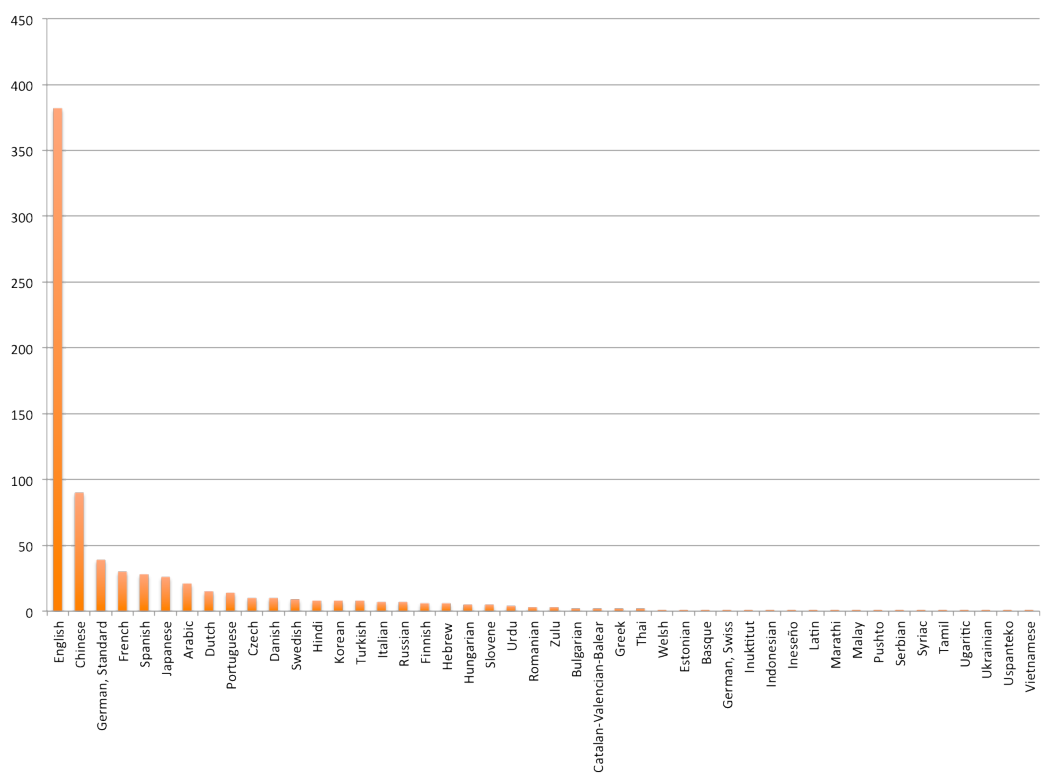
\includegraphics[width=0.71\textwidth]{../_media/Languages-in-LT-Research}
  \caption{Languages treated in research published in the 2010 edition of the Journal of Computational Linguistics and the conferences of ACL, EMNLP and COLING (internal, unpublished study)}
  \label{fig:languages-in-research}
  \colorrule{grey3}{\textwidth}{1.5pt}
\end{figure*}

Research activities have tended to be isolated, delivering valuable results, often failing to make a decisive impact on the market. In many cases research funded in Europe eventually bore fruit outside Europe. Companies such as Google and Apple have been noteworthy beneficiaries. In fact, many of the predominant actors in the field today are enterprises based in the United States.

%%%%%%%
%
% This bit commented out as suggested by Volker Steinbiss et al.
%
%Statistical methods have been succesful, scaling to many languages and application domains but in many cases reached a performance plateau and inclusion of and combination with deep linguistic methods and insights is seen as a promising a way forward.
%
%In the pure statistical approach, sentences are automatically translated by comparing each new sentence against thousands of sentences previously translated by humans; the quality of the output largely depends on the size and quality of the available data. While the automatic translation of simple sentences in languages with sufficient amounts of available textual data can achieve useful results, statistical methods are likely to fail in the case of languages with a much smaller body of sample data or in the case of new sentences with complex structures. Analysing the deeper structural properties of languages is a promising avenue if we want to build applications that perform well across the entire range of European languages.
%
%%%%%%%

Europe now has a well-developed research base. Through initiatives such as CLARIN and META-NET the research community is well-connected and engaged in a long term agenda that aims gradually to strengthen language technology's role. Yet at the same time, our position is worse when compared to other multilingual societies. Despite fewer financial resources, countries like India (22 official languages) and South Africa (11 official languages) have set up long-term national programmes for language research and technology development. What is missing in Europe is awareness, political determination and courage that would take us to a leading position in this technology area through a concerted funding effort. This major dedicated push needs to include the EU-wide political determination to modify and to adopt a shared, EU-wide language policy that foresees an important role for language technologies. 

Drawing on the insights gained so far, today’s hybrid language technology mixing deep processing with statistical methods could be able to bridge the gap between all European languages and beyond. In the end, high-quality language technology will be a must for all of Europe's languages for supporting the political and economic unity through cultural diversity. Language technology can help tear down existing barriers and build bridges between Europe’s languages. In the digital age, communication with people and machines, as well as the unrestricted access to the knowledge of the world should be possible for all languages. The European LT community is dedicated to fulfilling the technology demands of the multilingual European society and to turn these needs and emerging business opportunities into competitive advantages. To this end, we have developed this Strategic Research Agenda (see Appendix~\ref{vision-evolution}, p.~\pageref{vision-evolution}).

In the first chapters we analyse the multilingual technology needs arising from the multicultural setup of our continent with its emerging single digital market. We also discuss the current state of technologies for European languages. The two core chapters of this document summarise our shared vision of the role of language technology in the year 2020 in non-technical terms (Chapter~\ref{sec:lt2020}, p.~\pageref{sec:lt2020}\,ff.) and outline three priority themes for large-scale research and innovation (Chapter~\ref{sec:pts}, p.~\pageref{sec:pts}\,ff.):

\begin{enumerate}
\item \textbf{Translation Cloud} -- Services for instantaneous reliable spoken and written translation among all European and major non-European languages
\item \textbf{Social Intelligence and e-Participation} -- understanding and dialogue within and across communities of citizens, customers, clients, consumers
\item \textbf{Socially Aware Interactive Assistants} -- analysis and synthesis of non-verbal, speech and semantic signals
\end{enumerate}
 
These thematic directions have been designed with the aim of turning our joint vision into reality and to letting Europe benefit from a technological revolution that will overcome barriers of understanding between people of different languages, between people and technology and between people and the accumulated knowledge of mankind. The themes build the bridge between societal needs, applications, and roadmaps for the organisation of research, development and scientific innovation. They cover the main functions of language: storing, sharing and using information and knowledge, as well as improving social interaction among humans and enabling social interaction between humans and technology. As multilingualism is at the core of European culture and becoming a global norm, one theme is devoted to overcoming language barriers.

We also present ways in which research and innovation need to be organised in order to achieve the targeted breakthroughs and to benefit from the immense economic opportunities they create. Core components of the sketched strategy are novel modes of large-scale collective research and interaction among the major stakeholder constituencies including research in several disciplines, technology providers, technology users, policy makers and language communities. Effective schemes for sharing resources such as data, computational language models and generic base technologies are also an integral part of our strategy. Of central importance is a rapid flow of intermediate results into commercially viable solutions of societal impact contributing to the fertile culture of technological, social and cultural innovation targeted by the Digital Agenda \cite{DA2010} and the programmes Connecting Europe Facility (CEF) \cite{CEF2011} and Horizon 2020 \cite{H2020}.

The three priority research themes are mainly aimed at Horizon 2020 (2014--2020). The more infrastructural aspects, platform design and implementation and concrete language technology services are aimed at CEF. Our suggestion for integrating multilingual technologies into the wider CEF framework is to develop innovative solutions that enable providers of online services to offer their content and services in as many EU languages as possible, in a most cost effective way. These are to include public services, commercial services and user-generated content. An integral component of our strategic plans are the member states and associated countries: it is of utmost importance to set up, under the overall umbrella of our SRA and priority research themes, a coordinated initiative both on the national (member states, regions, associated countries) and international level (EC/EU), including research centres as well as small, medium and large enterprises who work on or with language technologies. Only through an agreement and update of our national and international language policy frameworks, close cooperation between all stakeholders, and tightly coordinated collaboration can we realise the ambituous plan of researching, designing, developing and putting into practice a European platform \cite{bruegel12} that supports all citizens of Europe, and beyond, by providing, among others, sophisticated services for communication across language barriers.  
\end{multicols}

\clearpage

% --------------------------------------------------------------------------

\ssection[Multilingual Europe: Facts, Challenges, Opportunities]{Multilingual Europe:\newline Facts, Challenges, Opportunities}

\begin{multicols}{2}

\subsection{Europe's Languages in the Networked Society}
\label{sec:status-europes-languages}

Europe’s more than 80 languages are one of its richest and most important cultural assets, and a vital part of its unique social model \cite{EC2,eurobarometer2012}. While languages such as English and Spanish are likely to thrive in the emerging digital marketplace, many European languages could become marginal in a networked society. This would weaken Europe’s global standing, and run counter to the goal of ensuring equal participation for every European citizen regardless of language. A recent UNESCO report on multilingualism states that languages are an essential medium for the enjoyment of fundamental rights, such as political expression, education and participation in society \cite{Unesco1}. From the very beginning, Europe had decided to keep its cultural and linguistic richness and diversity alive during the process of becoming an economic and political union. For maintaining the policy of multilingualism, the EU’s institutions spend about one billion Euros a year on translating texts and interpreting spoken communication. For all European economies the translation costs for compliance with the laws and regulations are much higher.

A single European market that secures wealth and social well-being is possible, but linguistic barriers still severely limit the free flow of goods, information, services, debates and innovation. With the increased number of EU members and the general trend towards timely trans-border interaction, everyday communication between Europe’s citizens, within business and among politicians is more and more becoming confronted with language barriers. Many Europeans find it difficult to interact with online services and participate in the digital economy. According to a recent study, 57\% of internet users in Europe purchase goods and services in languages that are not their native language (English is the most common foreign language followed by French, German and Spanish). 55\% of users read content in a foreign language while only 35\% use another language to write e-mails or post comments on the web \cite{EC1}. A few years ago, English might have been the lingua franca of the web -- the vast majority of content on the web was in English -- but the situation has now drastically changed. The amount of online content in other European as well as Asian and Middle Eastern languages has exploded \cite{Ford11}. Already today, more than 55\% of web-based content is not in English. One language is especially becoming more and more dominant: a recent study by the UN Broadband Commission reports that Chinese internet users will overtake English language users by 2015 \cite{chinese2012}.

Figure~\ref{fig:european-languages-in-twitter} shows the European language communities of Twitter: the map was created by identifying automatically the languages millions of tweets are written in and placing them onto a map using their GPS-coordinates \cite{fisher11}. To a large degree the resulting map replicates Europe's language borders -- and barriers.

% Figure removed, it doesn't add anything. Suggestion by Peter Spyns.
% 
%\begin{figure*}[htb]
%  \colorrule{grey3}{\textwidth}{1.5pt}
%  \center
%  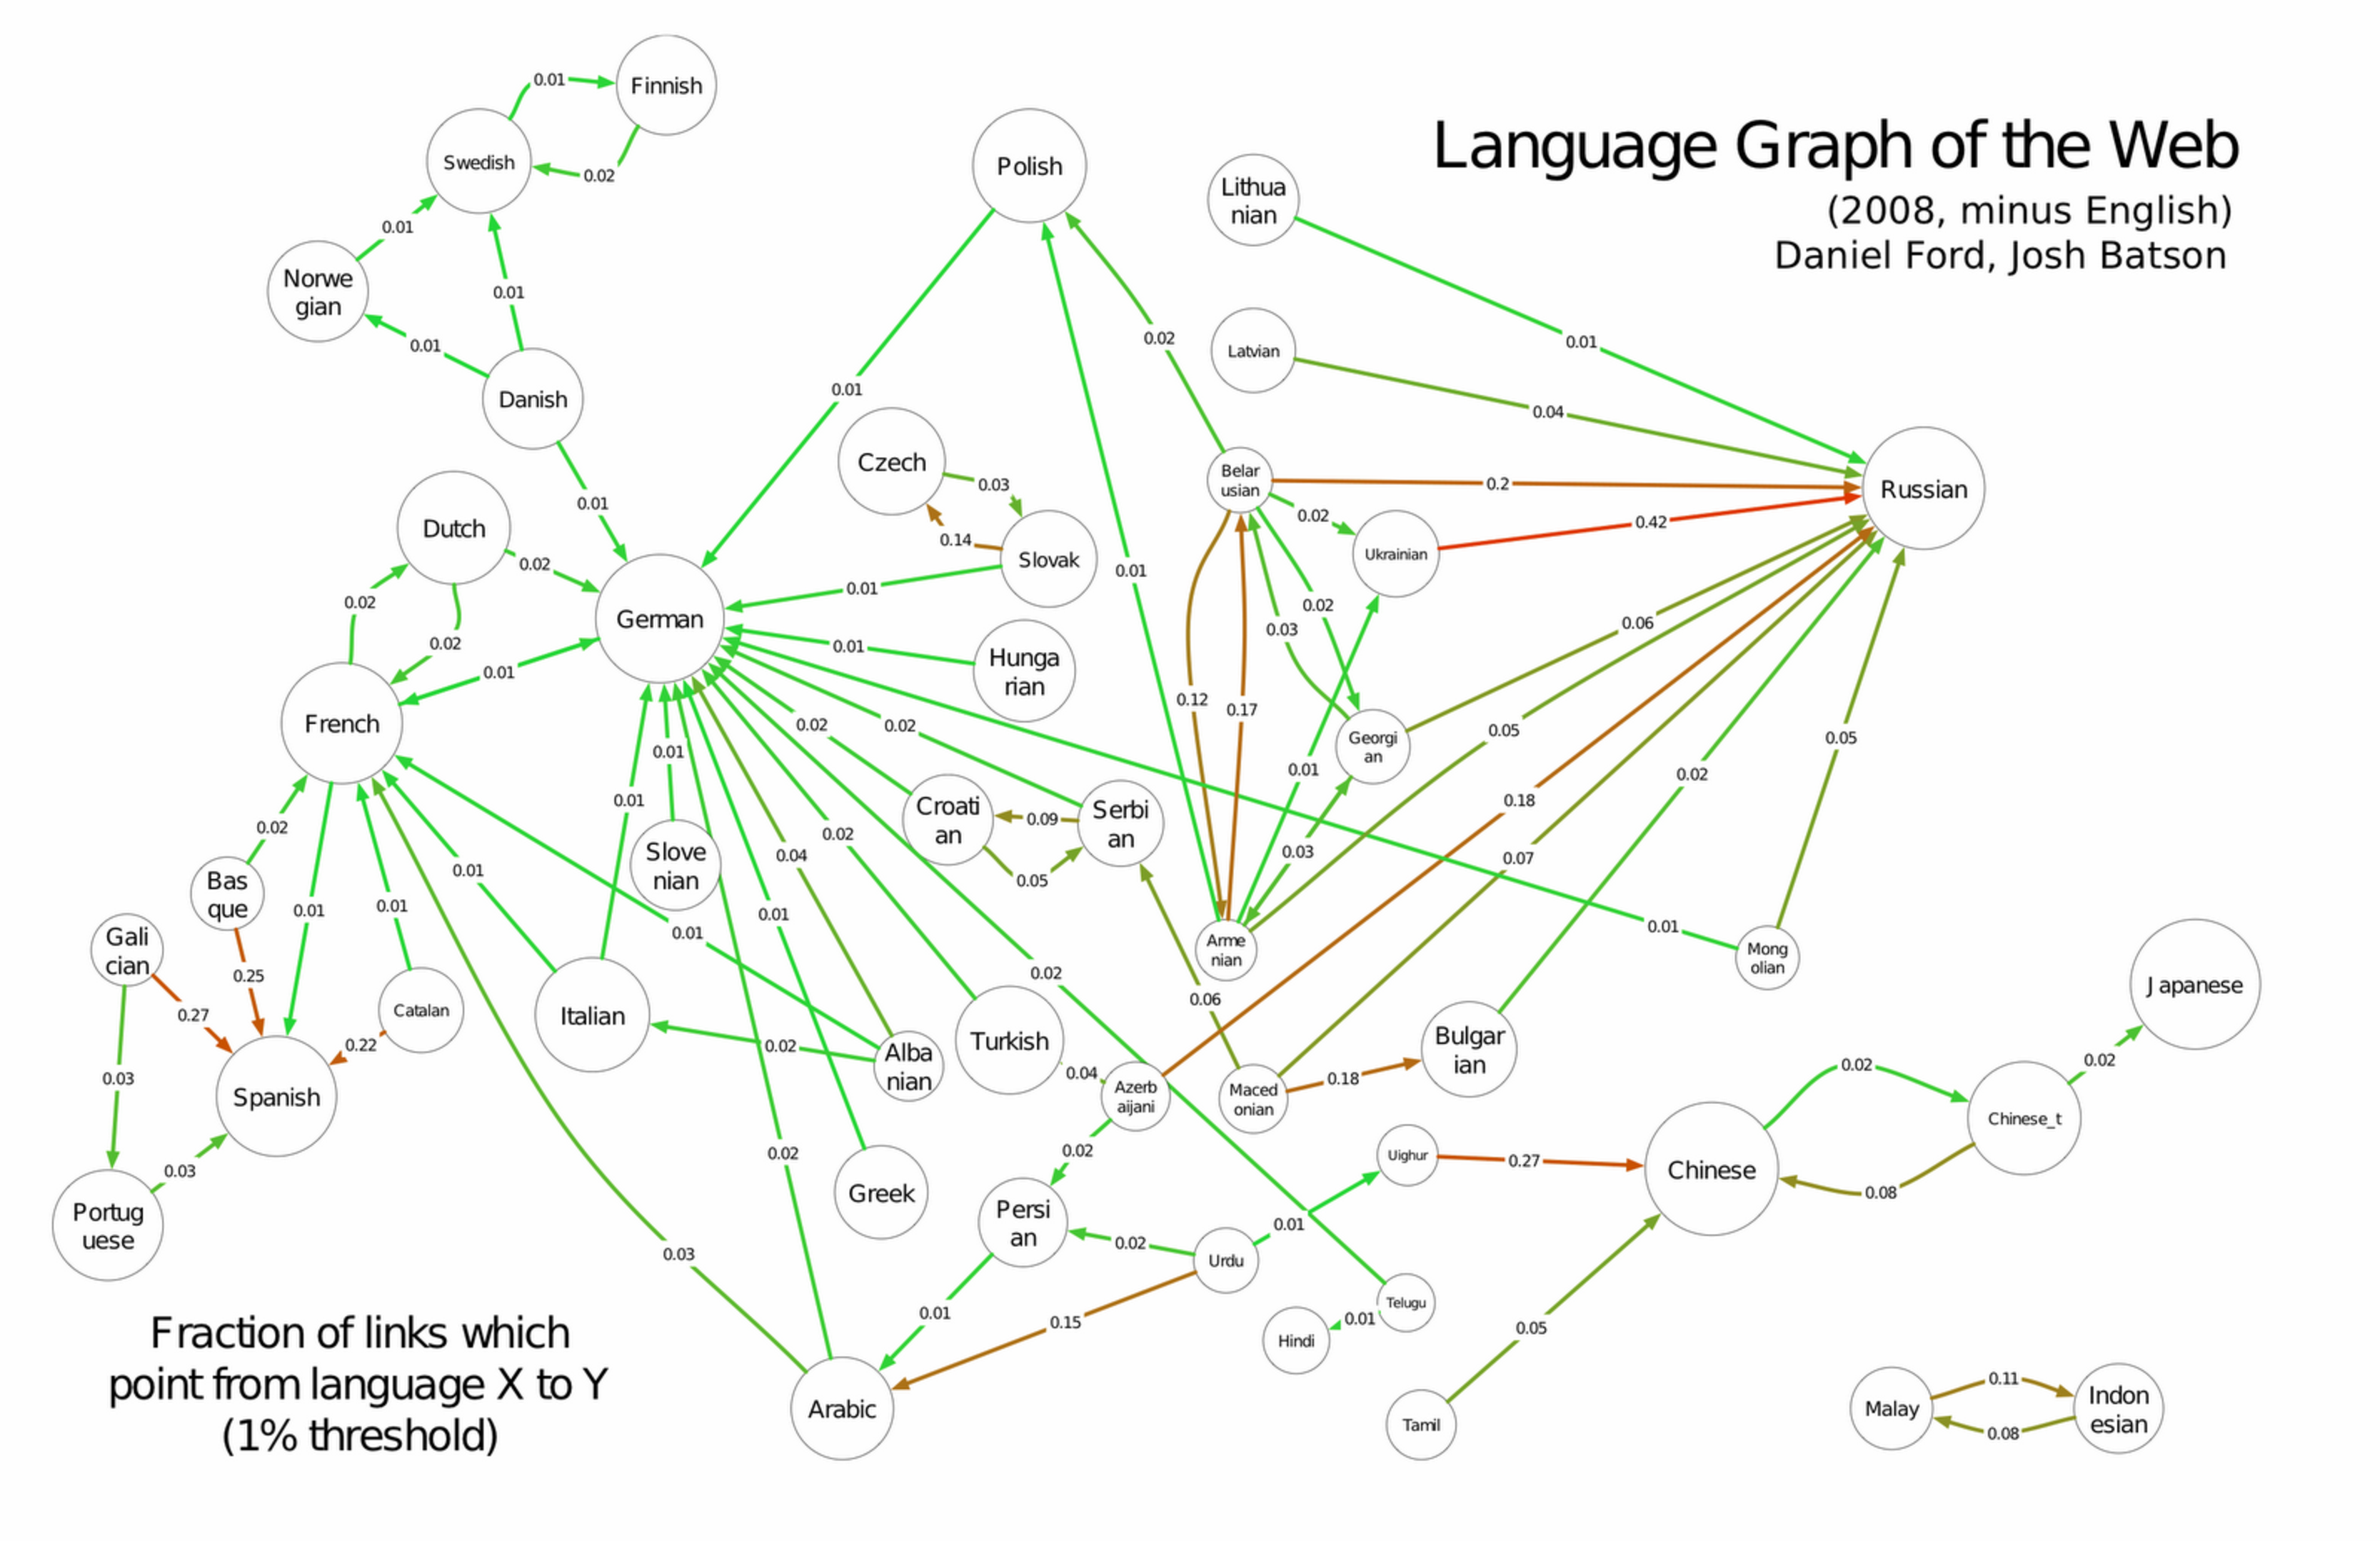
\includegraphics[width=0.9\textwidth]{../_media/Language-Graph}
%  \caption{Language graph of the web}
%  \label{fig:language-graph-of-the-web}
%  \colorrule{grey3}{\textwidth}{1.5pt}
%\end{figure*}

\begin{figure*}[htb]
  \colorrule{grey3}{\textwidth}{1.5pt}
  \center
  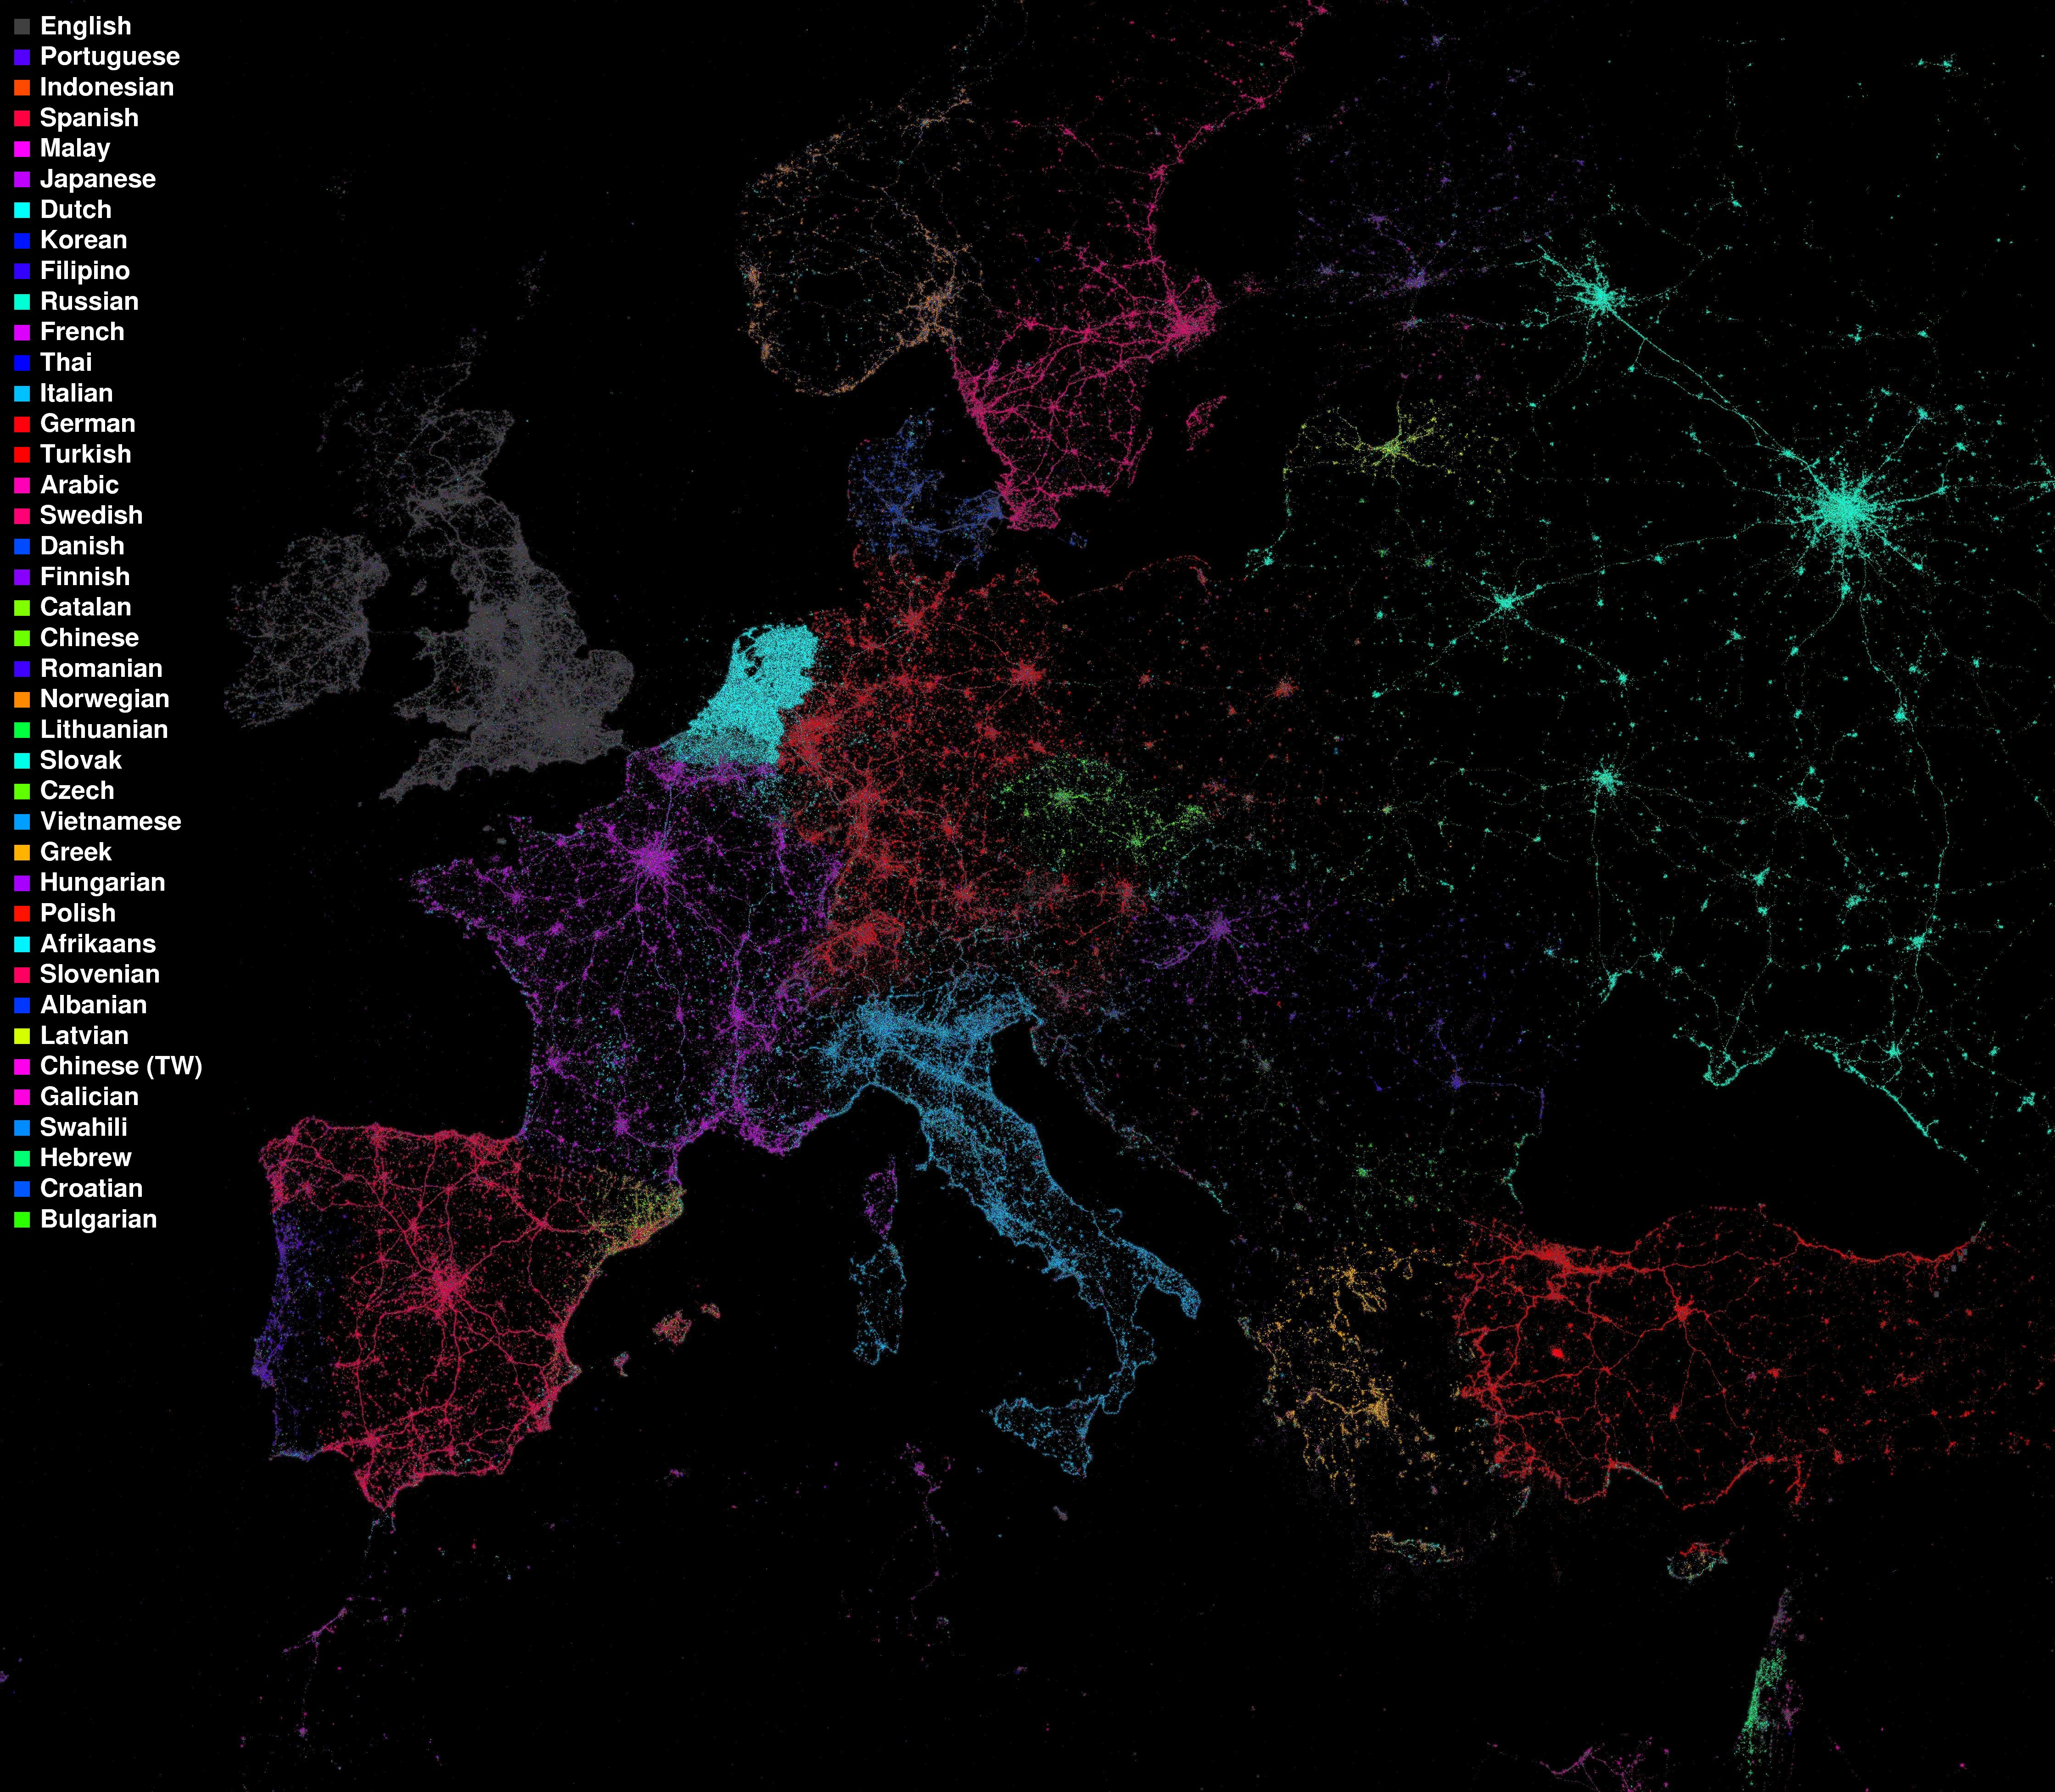
\includegraphics[width=0.9\textwidth]{../_media/twitter-languages-europe}
  \caption{Language communities of Twitter (European detail)}
  \label{fig:european-languages-in-twitter}
  \colorrule{grey3}{\textwidth}{1.5pt}
\end{figure*}

Surprisingly, this ubiquitous digital divide due to language borders and language barriers has not gained much public attention up until our recent press campaign in which we informed the public about the findings of our META-NET study ``Europe's Languages in the Digital Age'' (see Chapter~\ref{sec:lwp}, p.~\pageref{sec:lwp}\,ff.). In this study, published in our META-NET White Paper Series \cite{LWP2012}, more than 200 experts from all over Europe found that at least 21 of the 30 languages examined are in serious danger of facing digital extinction. A pressing question raises: which European languages will thrive in the networked information society, and which are doomed to disappear?

The European market for translation, interpretation and localisation was estimated to be 5.7 billion Euros in 2008. The subtitling and dubbing sector was at 633 million Euros, language teaching at 1.6 billion Euros. The overall value of the European language industry was estimated at 8.4 billion Euros and expected to grow by 10\% per year, i.\,e., resulting in approx.~16.5 billion Euros in 2015 \cite{EC3}. Yet, this existing capacity is not enough to satisfy current and future needs, e.\,g., with regard to translation \cite{csa2009}. Already today, Google Translate translates about the same volume per day that all human translators on the planet translate in one year \cite{och12}.

Despite recent improvements, the quality, usability and integration of machine translation into other online services is far from what is needed. If we rely on existing technologies, automated translation and the ability to process a variety of content in a variety of languages -- a key requirement for the future internet -- will be impossible. The same applies to information services, document services, media industries, digital archives and language teaching. There is an urgent need for innovative technologies that help save costs while offering faster and better language services to the European citizen.

The most compelling solution for ensuring the breadth and depth of language usage in tomorrow's Europe is to use appropriate technology. Still, despite recent improvements, the quality and usability of current technologies is far from what is needed. The META-NET study mentioned above shows that, already today, especially the smaller European languages suffer severely from under-representation in the digital realm. There are tremendous deficits in technology support and significant research gaps for all languages. For example, machine translation support for 23 out of the studied 30 languages was evaluated as having very limited quality and performance, which is an alarming result!

\subsection{How can Language Technology help?}
\label{sec:how-can-language-technology-help}

One way to overcome language barriers is to learn foreign languages. Yet without technological support, mastering the EU's 23 official languages and some 60 other European languages is an insurmountable obstacle for Europe’s citizens, economy, scientific progress, and political debate \cite{ombudsman2012}. The solution is to build key enabling technologies: language technologies will offer all European stakeholders tremendous advantages and benefits, not only in the single market, but also in trade relations with non-European countries.

Language technology is also a key enabler for the knowledge society. It supports humans in everyday tasks, such as writing e-mails, searching for information online or booking a flight. It is often used behind the scenes of other software applications. We benefit when we use spelling checkers, browse recommendations in an online shop, hear the spoken instructions of a navigation system or translate web pages with an online service.

Several popular language technology services are provided by US companies, some of them free of charge. The recent success of Watson, an IBM computer system that won against human candidates in the game show Jeopardy, illustrates the immense potential. As Europeans, we urgently have to ask ourselves a few crucial questions:

\begin{itemize}
\item Can we afford our information, communication and knowledge infrastructure to be highly dependent upon monopolistic services provided by US companies (technological lock-in)?
\item What is Europe's fallback plan in case the language-related services provided by US companies that we rely upon are suddenly switched off or if serious access or security issues arise?
\item Are we actively making an effort to compete in the global landscape for research and development in language technology?
\item Can we expect third parties from other continents to solve our translation and knowledge management problems in a way that suits our specific communicative, societal and cultural needs?
\item Can the European cultural background help shape the knowledge society by offering better, more secure, more precise, more innovative and more robust high-quality language technology?
\end{itemize}

We believe that \emph{Language Technology made in Europe for Europe} will significantly contribute to future European cross-border and cross-language communication, economic growth \cite{economist12} and social stability while establishing for Europe a worldwide, leading position in technology innovation, securing Europe's future as a world-wide trader and exporter of goods, services and information.

\subsection{Societal Challenges}
\label{sec:what-soci-challenges}

Information technology is bringing people speaking different languages together in new ways. Highly popular social networks and social media such as Wikipedia, Facebook, Twitter, YouTube, Google+, Pinterest, and Instagram are only the tip of the iceberg.

Many societal changes and economic as well as technological trends confirm the urgent need to include sophisticated language technology in our European ICT infrastructure. Research, development and innovation efforts in LT must increase to go beyond what is possible today.

\textbf{Language Barriers.} A study on online commerce shows that language barriers are economic barriers \cite{EC4}. Only 59\% of retailers can handle transactions in more than one language. Translation and localisation costs must be drastically lowered before Europe’s single digital market is a reality. Multilingual language technology is the key, especially for SMEs. At the same time, 81\% of all internet users think that websites run in their country should also be available in other languages. 44\% of European users think they miss out on interesting information because websites are not available in a language they understand \cite{EC1}. These facts can no longer be ignored. Reliable LT can help establish a vast market for information as well as consumer and entertainment goods in any language.

\textbf{Ageing Population.} Demographic changes bring about a need for more assistive technologies, especially for spoken language access. An ageing population requires technology that can help master everyday situations, provide proactive guidance and that could answer the question, “Where did I leave my glasses?” Also, more health care services and support systems will be required. Ambient assisted living (AAL) technologies can greatly benefit from a personalised, spoken method of interaction.

\textbf{People with Disabilities.} New technologies can help us reach the ambitious goal of achieving equal opportunities and promoting independent living. Language technologies already help people with disabilities to participate in society. Noteworthy examples include screen readers, dictation systems and voice-activated services. In addition to the social aspect there is a huge commercial market for future technologies such as, for example, full dialogue systems and interactive assistants, sign language recognition and synthesis, automatic translation, summarisation and content simplification. Approximately 10\% of Europeans (50 million citizens) have permanent disabilities.

\textbf{Immigration and Integration.} According to the United Nations' International Migration Report 2002, 56 million migrants lived in Europe in 2000 \cite{UN1}. This number has grown to ca.~60 million people today. Facilitating communication, providing access to information in foreign languages and helping people learn European languages can help better integrate migrants into European society. In fact, speech and language technologies can dramatically improve the integration process by providing intelligent language learning environments, automatic subtitling and translation services in real time.

\textbf{Personal Information Services and Customer Care.} In our 24/7 ``always on'' economy we expect quick and reliable answers as well as engaging and timely online news broadcasts. However, information overload still poses a serious problem. Citizens, governments and industries would greatly benefit from new technologies that help get the situation under control again. Language-enabled mobile applications will become personal assistants to everyone, offering automatic and intelligent question answering and dialogue capabilities, as well as automatic, personalised and trusted text and speech processing of messages, news items and other content.

\textbf{Global Cooperation and Human Communication.} Companies need to address new markets where multiple languages are spoken and support multinational teams at multiple locations. Many jobs cannot be filled today because linguistic barriers exclude otherwise qualified personnel. Improvements in language technology can enable richer interactions and provide more advanced tele and video conferencing services. Future technologies like a 3D internet can enable new modes of collaboration as well as support more realistic training and education scenarios. We will soon be able to participate in virtual events as new forms of entertainment, cultural exchange and tourism. Combining virtual worlds and simulations with multilingual language technology including translation, automatic minute taking, video indexing and searching will let us experience being European in a new way.

\textbf{Preservation of Cultural Heritage and Linguistic Diversity.} According to the principles of the UN-endorsed World Summit on the Information Society \cite{worldsummit2003}, the “Information Society should be founded on and stimulate respect for cultural identity, cultural and linguistic diversity.” Much effort has been put into the creation of digital archives such as Europeana that help promote our cultural heritage. However, digitisation is only the first step. The sheer amount of information and language barriers hinder access of our cultural treasures. Language technology can make this content accessible, e.\,g., through cross-lingual and multimedia search and machine translation. Likewise, communication skills need to be trained. This is underlined by the UNESCO Information for All Programme \cite{Unesco2}, which seeks to “foster the availability of indigenous knowledge through basic literacy and ICT literacy training.”

\textbf{Social Media and e-Participation.} Social networks have a significant impact on all areas of society and life. They can help us solve technical problems, research products, learn about interesting places or discover new recipes. Recent developments in North Africa demonstrate their ability to bring citizens together to express political power. Social media will play a key role in the discussion of important, future topics for Europe like a common energy strategy and foreign policy. However, certain groups are becoming detached from these developments. One can even speak of a broken link regarding communication cultures. This is an issue since bottom-up movements are highly relevant for politicians, marketing experts, and journalists who would like to know what customers or citizens think about initiatives, products, or publications. However, it is not possible to process manually the sheer amount of information generated in multiple languages on social networks. We need language technologies that are able to analyse these streams in real time.

\textbf{Market Awareness and Customer Acceptance.} Language technology is a key part of business and consumer software but often hidden inside other, more visible products. Customer acceptance of LT has recently been shown to be high. For example, market research by the Ford Motor Company indicates that their voice control system, Ford SYNC, is widely accepted \cite{ford}. 60\% of Ford vehicle owners use voice commands in their cars. Non-Ford owners report a three-fold increase in their willingness to consider Ford models while 32\% of existing customers admit that the technology played an important role in their purchase decision. Language technology has a tremendous market potential.

\textbf{One Market, Many Languages.} Support for the 23 official languages of the EU has major economic, social and political implications. Europe currently lags behind countries such as India (22 official languages) and South Africa (11 national languages). Government programmes in these two countries actively foster the development of language technology for a significant number of official languages \cite{india2012,sa2012}. Mobile devices are an even more important bridge between humans and information technology. Google already provides free translation services in 3,306 different language pairs as well as voice input for 16 languages and speech output for 24 languages. Apple's App Store has demonstrated how premium content and products can be marketed for free and for a fee. Europe must address this global competition.

\textbf{Secure Europe.} The effective persecution of illegal online activities such as fraud and identity theft requires automatic tools that can help detect crimes and monitor offenders. Language technology can help to build systems that can monitor, analyse and summarise large amounts of text, audio and video data in different languages and from different sources.

This collection of solutions was influenced by bigger trends (see Chapter~\ref{sec:ict-trends}). Many of these products and services are only available online. For example, Facebook and Twitter enabled recent political developments in North Africa. In Europe, the idea of social innovation has recently sparked an interest as it “offers an effective approach to respond to social challenges by mobilizing people's creativity to develop solutions and make a better use of scarce resources” \cite{EC5}. Social innovation is part of Europe’s 2020 strategy and critically relies on active involvement of citizens, which in turn calls for supportive multilingual language technologies.

Multilingualism has become the global norm rather than the exception. Future applications that embed information and communication technology require sophisticated language technologies. Fully speech-enabled autonomous robots could help in disaster areas by rescuing travellers trapped in vehicles or by giving first aid. Language technology can significantly contribute towards improving social inclusion. Language technology can help us provide answers to urgent social challenges while creating genuine business opportunities.  Language technology can now automate the very processes of translation, content production, and knowledge management for all European languages. It can also empower intuitive language/speech-based interfaces for household electronics, machinery, vehicles, computers and robots

In addition to these vertical societal challenges there are multiple horizontal properties that future language technologies need to exhibit. One of these properties is situation or context awareness. Many or even most applications sketched above need to exhibit a certain level of situation or context awareness. The challenge is to design and implement a paradigm in which language technologies are no longer static applications but able to adapt themselves to specific situations, trends and contexts such as, for example, user preferences or user interests. Security applications need to be aware of criminal or violent tendencies in communication patterns. E-participation systems need to be aware of interest in societal issues and need to have access to internet debates and the opinion of large online communities towards certain topics. Tools for the analysis of market awareness need methods for reputation mining, customer relationship systems need algorithms for attitude analysis.

\subsection{Market Opportunities}
\label{sec:market-opportunities}

% FIXME: This subsection is no longer repeated. The other one was deleted.
%
% FIXME: This subsection needs to be extended with Rose Lockwood's new content.

There is an immensely large set of promising market opportunities around language technologies in Europe. We agreed with the EC-funded initiative ``LT Innovate'' (``LT-Innovate is the Forum for Europe's Language Technology Industry'', see \url{http://lt-innovate.eu}) that we will include a concise description of the market opportunities into this document once the ``LT Innovation Agenda'' has been prepared.

To provide a rough indication about the estimated size of the different markets: The European market for translation, interpretation and localisation is expected to have a size of ca.~16.5 billion Euros in 2015 \cite{EC3}. The global speech technology market is to reach the number of ca.~20.9 billion US-Dollars by 2015 and ca.~31.3 billion US-Dollars by 2017 \cite{gia2012}. In addition, it is often said that only a very small fraction -- about 0.5\% -- of what needs to be translated today is currently being translated due to cost and time constraints. Humans cost too much and take too long.
\end{multicols}

\clearpage

% --------------------------------------------------------------------------

\ssection[Major Trends in Information and Communication Technologies]{Major Trends in Information and Communication Technologies}

\begin{multicols}{2}

\subsection{The Current State}
\label{sec:ict-trends}

% FIXME: Important aspects from \cite{bruegel12}:
%
% "Europe's failure to specialise in new ICT sectors and firms is likely to hold back Europe’s post-crisis recovery. Europe lacks in particular leading platform providers, who are capturing most of the value in the new ICT ecosystem."
%
% "In-depth analysis of some specific new emerging ICT sectors shows that the problem in Europe appears not to be so much in the generation of new ideas, but rather in brin- ging ideas successfully to market. Among the barriers are the lack of a single digital market, fragmented intellectual property regimes, lack of an entrepreneurial culture, limited access to risk capital and an absence of ICT clusters."
%
% "The EU policy framework, particularly the Innovation Union and Digital Agenda EU 2020 Flagships, could better leverage the growth power for Europe of new ICT markets. The emphasis should move beyond providing support for infrastructure and research, to funding programmes for pre-commercial projects. But perhaps most important is dealing with the fragmentation in European digital markets."

Networked computers are ubiquitous. They come in many different shapes and forms (desktop, laptop, mobiles, tablets, etc.) or are embedded in devices, objects, and systems (e.\,g., smartphones, cameras, washing machines, cars, heating systems, robots, factories, traffic control systems). Software is usually available in multiple human languages. Standardisation efforts such as the introduction of Unicode solved the problem of representing and displaying different scripts, alphabets and special characters. The main use cases for today's computers are text processing, spreadsheets, presentations, communication (e-mail, Facebook, Twitter, Skype etc.), information search and entertainment (photos, music, films, games).

Mobile devices and social media are ever more reshaping how and when we communicate with one another using the tools and devices we use both in business and private life. The way we interact with computers is no longer restricted to graphical user interfaces with limited functionality but it is being extended through touch screens, voice interfaces and dialogue systems, tactile interfaces and mobile devices with built-in accelerometers that tell the device how it is held by the user.

Language technology is currently not well integrated into applications and interfaces -- to the end user, spelling and grammar checking as well as, to a certain extent, search seem to be the only notable exceptions. A trend towards more intelligent language-based interaction is illustrated by Apple’s introduction of the mobile assistant Siri in the latest iPhone and, recently, Google Now.

The web represents much of our knowledge. It emerged as a collection of static documents. Nowadays it is first and foremost a collection of systems and databases that can be queried through APIs, and applications such as Google Mail, Google Calendar, Facebook, eBay and Amazon. Many people only need one interface application on their computers: a web browser. Others use netbooks whose operating system more or less \emph{is} the browser (Chromium OS). Behind the scenes, there is already a considerable amount of language technology incorporated in web applications such as search engines, dialogue systems, or machine translation services.

% =========================================================================================

\subsection{Hardware and Software}
\label{sec:hardware-software}

Networked computers are no longer as big as a refrigerator, the age of the clumsy tower or desktop computer is over. Nowadays, networked computers come in many shapes and forms: small mobile devices (smartphones using, for example, Android or iOS), tablets, netbooks, ultra-portable laptops, small desktop computers, ebook readers, radios, television sets, gaming consoles and other entertainment devices with built-in wireless and access to, for example, RSS feeds, internet radio stations or youtube, cameras or house-hold appliances such as vacuum cleaners, coffee machines or scales that push the weight of the user to the cloud from where it can be monitored using an app on the smartphone. The next revolution in the hardware market will be wearable computers. Google has already demonstrated a prototype of their Google Glasses product in which the computer visuals are projected into a head-up display that looks like a regular pair of glasses. This approach can be used to provide the user with a true augmented reality perspective and a hands-free computing environment which immediately brings up the question if it will be possible to interact with the Glasses, or a similar product, using only your voice.

The shape and size of computers is no longer determined by the shape and size of their internal hardware components. Due to further breakthroughs in miniaturisation, the form of computers now truly follows their function. While computers and devices with embedded systems get smaller and smaller, the distributed data centres around the world get bigger and bigger -- both in terms of number and size. The concept of cloud computing and storing data in dedicated data centres from where the data can be accessed by multiple devices (see, for example, Apple's iCloud), is already mainstream and used by millions of consumers world-wide. An important reason for the success of using the cloud to store data is the fact that, by now, people tend to have more than one computer, a not too unusual setup may include a laptop, a smartphone, a tablet and another computer as a dedicated media centre. Cloud services are ideal for synchronising data between all devices without buying, configuring and administering your own server machine.

The trends in the software area are much more multi-dimensional -- in this section we can only scratch the surface and highlight several recent developments and current trends.

\textbf{Communication:} Probably the most important cornerstone of today's computer use is communication (both human to human and human to machine), be it more direct communication via traditional e-mail, instant messaging, text-based chat systems, video chat between two people or larger groups (Skype, Facetime, Google Hangout) or indirect communication and staying in touch with friends, acquaintances and colleagues via social networks such as Twitter, Facebook, XING and LinkedIn or social media such as blogs, YouTube, Pinterest or Instagram. An important factor is that millions of people world-wide are, by now, always online using several different networked devices including their phones. 

\textbf{Search and Information Services:} Another important use case of any type of computing device is to search for information and to make use of specialised information services. Important applications are web search engines such as Google Search or Microsoft's Bing, Wikipedia, Google News, Google Books, digital libraries such as Europeana, meta-search engines and RSS feed aggregators etc.

% FIXME: Comment from Jussi Karlgren:
%
% MEDIA MONITORING as an technology in the software section
%
% i would also like to see media monitoring and situation awareness in general as an application in the 3.3 section. where "retrieval" is about finding stuff you already know about or suspect is there and "search" adds exploration to "retrieval" they both are about finding the needles in the haystack or the gold nuggets in the sand. situation awareness is different - it is not about finding a document or an item - it is about keeping track of the state of the world. applications for this purpose are coming to the market at a rapid pace under various descriptive names such as "monitoring" and "mining" and many of them are indeed based on language technology!

\textbf{Location-based Services:} Search queries are nowadays often coupled to the user's current location. Location-based services enable the user to search for certain information in his or her geographic area, to make use of online maps, navigation systems, recommender systems such as Yelp or Qype or to find tweets or photos on Instagram in his or her geographic area.

\textbf{E-Commerce and Shopping:} World-wide billions of Euros are spent each year using general online shops such as Amazon or eBay or shops run by specific brands or services, reservation and booking, online banking and brokering services etc. 

\textbf{Media and Entertainment:} Different types of media (photos, videos, music, sounds, text and multimedia documents, audio and video podcasts, ebooks, films, tv programmes etc.) play an important role. Not only personal media and other user-generated content are often connected to social networks (posting photos or videos on Instagram, Facebook, Google+, Flickr or YouTube), songs, photos or videos created and posted by third parties are also often shared using social networks. Almost all of the media mentioned above can be purchased using general or specific online stores, for consumption on any device. Another important category of software is games, from online Flash games to games that are embedded into social networks, location-based games, multi-player games with millions of users to very simple but also very successful casual games such as Angry Birds.

\textbf{App and Media Stores:} The success of ecommerce platforms \cite{bruegel12}, online shopping and the increased use of digital media led to the development of dedicated app and media stores. By now it is possible to buy or to rent almost every movie ever made (Amazon, iTunes), to buy music (iTunes music store), to stream music from the cloud onto your device (Spotify) and to buy software and mobile apps through dedicated stores (e.\,g., Apple's app stores for MacOS and iOS) without any need to ship physical media. An important development is in-app purchasing, especially on mobile devices: with a single tap of a finger it is possible to buy, within a specific app (which is usually available for free), additional modules, components or data sets for a small price.

\textbf{Personal Information Management:} With the ever increasing number of personal and professional contacts (including social networks), meetings and personal errands to run, there is a big trend towards personal information management. This includes address and contacts databases that are often integrated into larger applications such as Google Contacts (embedded in, among others, Google Mail) or Apple's AddressBook (used in Apple Mail). Cloud-integration is an important feature, so that contact information (including names, email address, phone numbers, photos etc.), calendar entries, ``to do'' items and the data from other productivity tools are always available on all devices. 

\textbf{Office Applications:} The classic office applications --~word processors, spreadsheets, presentations~-- are still important in the professional context and also in home use. Nowadays, there are several applications to choose from including open source software, cloud-based services and applications for Apple's iOS (MS Office, Apple iWork, Open Office, Google Docs). Except for Open Office all office suites use the cloud to enable the user to, for example, finish work on a presentation at the desktop computer where the document is automatically pushed to the cloud and to continue working on the presentation on a mobile device on the way home.

One of the most basic common denominators of all pieces of software is language -- language plays a central and integral part in practically every single app, tool or application. However, language technology as such (including text analysis, information retrieval and extraction, spelling and grammar checking, speech recognition and synthesis, dialogue systems etc.)~is usually completely hidden from the user, integrated into bigger applications, working behind the scenes. There is, however, a clear trend to embed language technologies not only at the level of the single application but on the level of the operating system. Another important factor of current computing is communicating and interacting with other people or groups of people, both on the personal level and also for business purposes.  A third crucial ingredient of computing today is information, especially structured information which is annotated based on specific standards (see, for example, the family of standards around XML, Semantic Web, Linked Open Data, Web Services etc.).

\subsection{Current Trends and Mega-Trends}
\label{sec:major-trends}

% FIXME: Koenraad De Smedt on this section: "Section 3.4 is mostly superfluous.  Sentences like "New business models and ways to distribute content or services to the end-user will continue to emerge" are unneccessary and sentences like "web search is generally considered a solved problem" are in need of serious qualification."

In the following we briefly sketch some of the current trends and mega-trends, loosely grouped into three sections.

\textbf{Internet:} The internet will continue to be \emph{the} main driving force behind future developments in information and communication technologies. There are several mega-trends tightly coupled to the internet and network technologies: among these are cloud computing and cloud services, including cloud storage, as well as linked open data and the semantic web. Social media and social networks will continue to change everything and to penetrate the market further, including niche markets, driven by location-based services. With the predominance of social networks we expect a certain convergence of digital identities that will enable users to have and to maintain one central digital identity that feeds into their multiple social network profiles including also a merger of the business-self and the private-self. Along those lines, exchanging and distributing personal data and information (photos, videos, music etc.) in a secure way will become easier. We further expect more broad deployment and general acceptance of services in the areas of e-democracy and e-government (including open data portals) and a continued increase of e-commerce platforms \cite{bruegel12} and services. A perceived general information overload will continue to be a problem, although modern search engines, aggregation services and user interfaces help a lot; web search is generally considered a solved problem. New business models and ways to distribute content or services to the end-user will continue to emerge (see the different app stores and approaches such as in-app purchases).

\textbf{People:} Information and communication technologies are used by people -- the predominance of social networks and being always-on using smartphones, tables and laptops, is responsible for the fact that the way people interact, communicate and do business with one another will continue to be redefined and reshaped completely, including novel approaches for participation and public deliberation processes. Communication tools such as email, Twitter, Facebook etc.~are mainstream by now and used across all age groups. This trend will continue. A popular phrase that characterises the main essence of the success factor of social networks is ``faces and places'' as this is what people are mainly interested in: other people first and foremost as well as certain buildings, restaurants, cinemas, landmarks and many others. The trend to use location-based services to find current friends, items of interest or even new friends with similar interests on social networks will continue (along with a more in-depth discussion of privacy issues). We also expect a tighter connection between the data stored in social networks and the linked open data cloud as well as a tighter connection between tools for personal information management and linked open data.

\textbf{Hardware and Software:} By now many internet companies operate under the slogan ``mobile first''. Accessing the internet or using web services on mobile devices will overtake the use of desktops and laptops very soon. There is also a clear tendency for completely novel mobile devices with Apple's iPad and Google's Glasses being two prime examples; in addition, there is a tendency for more household-appliances connected to the internet (tv, radio, gaming consoles, refrigerator, scales, coffee machine, lamps etc.; see the Internet of Things). Many of these devices will not have any displays but voice-driven interfaces. We expect a seamless integration of mobile devices into the hardware landscape at home including very simple file, data and application transfer and exchange among arbitrary mobile or stationary devices, playing music or movies on arbitrary displays or video projectors etc. Very soon there will not be a need anymore for the average user to own a laptop or desktop computer because mobile devices (phones and tablets) will cover all basic needs. As regards networks, their capacity and bandwidth will continue to grow, mobile telecommunication networks will gradually become more important than, for example, ADSL lines. The quality of voice or video calls (Skype, Facetime, Google Hangout) will continue to improve, phones and all other devices will continue to become faster, have more storage as well as 3D-capable displays that offer more intricate modes of interacting with the device. Mobile phones will have built-in facilities to replace credit cards for payment purposes (for example, using Near Field Communication), effectively replacing the wallet. Finally, the market for apps, especially mobile apps, will continue to grow. Nowadays many companies, services and events have their own app that users can interact with and that usually offer added value when compared to the respective website. In order to be successful on the app market, usability will continue to be a decisive factor: only those apps will be successful that users can interact with intuitively right away.

To sum up, information and communication technologies will continue to be ubiquitous, available wherever and whenever needed. These technologies will be services that combine widely distributed applications, resources and data. They will be able to adapt to the location, situation and needs of the user including current emotions, habits and goals. As can be seen by the success of Wikipedia and other collaboratively edited knowledge bases, it is only a matter of time until a gigantic digital model of our world (or a multitude of bigger and smaller digital models) will exist that consists of interlinked and overlapping components. Naturally, languages and especially the automatic processing of languages using sophisticated language technologies will play a key role in this development. Now is the time to realise the needed breakthroughs. High performance, robust machine translation and related language technology services are urgently needed. There is a huge window of opportunity for consumer-oriented language technology: mobile devices are fast enough and have enough computing power, memory and a direct internet connection; they have a camera and are always online; it is easy to buy apps or add-ons.

While the LT-related aspects will be further discussed in the following chapters, we provide a more in-depth discussion of three selected trends in Sections~\ref{sec:linked-data-open}--\ref{sec:cloud-sky-computing}.

\subsection[Selected Trend: Linked Open Data and the Data Challenge]{Selected Trend:\newline Linked Open Data and the Data Challenge}
\label{sec:linked-data-open}

Data is considered one of the main topics of the future. At the European Data Forum 2012 and several other occasions the ``data challenge'' (big data, open data, linked data and the data value chain) is seen as one of the main themes and driving forces for future developments in information technology. Language technology and the priority research themes described later have strong relations to the data challenge, both as contributors and as beneficiaries. On the one hand, LT can help to exploit the immense volumes of information, knowledge and data encoded through natural language in text documents. LT can extract information from texts and make them accessible as structured data for automatic processing. On the other hand, LT will be able to analyse and interpret language data much better if it can use the growing volume of available structured data as background knowledge. 
%
Most of humankind's knowledge, reflection, communication and planning is encoded in and through human language. Conceptualising language as an integral part of the growing data universe is the ultimate challenge for the “big data movement”. Interpreting and interlinking textual knowledge with the linked data world will help in the process of extracting new knowledge from the masses of newly produced structured data.

The Translation Cloud will benefit from data available across languages. The translation technologies being developed will also help to address data challenges, like building and cleaning data sets that span across languages or building links between existing data sets within one or between several languages. Multilingual access is an important requirement for a European vision of e-Government and e-Participation services. On the one hand, language technology can make use of open, governmental data that is being developed in portals like data.gov.uk or within the upcoming European data portal. On the other, improving language technologies is inevitable for realizing multilingual access to public sector data for all European citizens, as recommended by the European Interoperability Framework for European public services \cite{EIF2010}: the sheer amount of data and language barriers between data sets are obstacles that can only be removed with technologies in the realm of, e.\,g., machine translation, cross-lingual information access and information extraction. Finally, one application scenario of Socially-Aware Interactive Assistants are multilingual virtual meetings that make use of shared data sets that provide information about individuals, organizations and interactions settings. The creation of these data sets is a challenge in terms of privacy and re-use of data. This leads to various open issues that need to be resolved both for the data challenge in general and for language technologies:

Public and private data infrastructures need to be made available with different implications in terms of, e.\,g., licensing schemes or provenance of data. Provenance in general is an important aspect to achieve trustworthiness of data and to assure data quality. The language technology community has created many language resources of high quality, and with adequate provenance information, these resources will play an important role for creating truly multilingual, linked open data. As a prerequisite, the data itself developed within language technology and localisation (terminological or lexical data, translation memories or language resources in general) needs to be made available as linked open data, using standardised, e.\,g., Semantic Web technologies. In addition, for creating applications based on these resources, language technologies need to be made ready-to-use beyond general textual input or output, for areas relying on quite specific formats like e-Government or e-Business.

% Following are the four new paragraphs to which Serge Gladkoff provided input.

There is another aspect of data in general that needs to be taken into account: From the perspective of human and machine translation workflows, and actually every LT application, there are two types of relevant data. The first are resources that are part of, e.\,g., an MT process: a statistical language model, rules for grammar-based machine translation, lexicons etc. The other are metadata, necessary to organize and improve translation or other LT-related processes. A big challenge for LT is the proliferation of formats and metadata types. The combination of input and output formats, of languages and domains to be taken into account, of customer relations in real-life scenarios and many others, lead to a multitude of problem situations that need to be solved individually.

The only way to tackle this problem is to develop standardised metadata which would help in various areas. First, workflows can be organised more easily, from source content through LT processes and back again, including CMS, TMS and CAT systems. Second, re-use of resources becomes easier by providing standardised metadata for identifying resources or pieces of content. Finally, metadata will foster interoperability of components in agile workflows, e.\,g., to ease the integration of the output of text analytics (e.\,g., standard tags for named entities) with terminology management and MT systems.

Metadata also need to be accompanied by reference implementations that help to achieve wide adoption. In addition, all metadata standardisation efforts need to involve not only consumers of metadata. It is important that producers of content are brought to the table; only high quality content with the appropriate metadata can lead to high quality results in LT applications.

With support from the 7th Framework Programme, the data and LT communities already have started building bridges in projects and infrastructures such as DBpedia, Monnet, Wikidata and META-SHARE. For the topic of metadata standardisation including LT, various organisations have proven to be helpful for wide range community building, including ISO TC~37, GALA and the World Wide Web Consortium (W3C). We are now in a good position to strengthen these relations and to assure the long-term availability of data and metadata for the European multilingual information society.

% FIXME: Important comments from Jussi Karlgren:
%
% this growth provides language technology with a great opportunity. you write quite eloquently about how human language is the prime knowledge repository and communication tool, but there is more to it than that! language is an open-ended communication protocol designed for incremental on-line learning without fixed elementa, ontologies and dtd:s to standardize it. 
%
% what we learn from processing language is the prime tool for processing the huge and intractable data streams that will come at us in the near future! we shouldn't miss the big data challenge and leave it to database and network engineers! 
%
% so what would i like to see in the text?
%
% COOPT THE BIG DATA CHALLENGE
%
% there is a bit on the big data challenge. that should be worded more aggressively. building future-proof solutions for big data analysis is *impossible* without language technology. big data analysis will not be slightly better if we include language technology - it simply won't happen. the human perceptual and language understanding components cope with big data, without pause, every waking hour. no problem there. we can't be downloading the big data we monitor on the internet into a database and then building applications on top of it - we will need to process it sensibly to begin with. and that sense will need to be based on language. in one sentence in the big data challenge you refer to "text documents". you should lift your vision a bit there - think about any sequential symbolic process of meaningful information! 
%
% BIG DATA LAYER IN THE SOFTWARE SECTION
%
% i would like to see a subsection in the 3.3 software section which discusses a general purpose processing layer for big data analysis. that is what we envision in the future of the technology we are building today with my colleagues at gavagai (http://www.gavagai.se). i would like to see a paragraph which says something about general purpose processing for human-generated data, an enabling technology for applications we do not have the imagination to sketch out today, the opportunities we hope to see future innovators, entrepreneurs and researchers be isnpired by and base their work on. (possibly this comment can be used to boost the bit on "cloud" there).

% FIXME: Comment from Christian Dugast concerning "Big Semantics":
%
% But language technologies allow to address much more than only communication solutions (talking, searching, translating ...).They also allow addressing data structuring solutions in order to organise, categorise, give meaning to data. More than 80% of the information available is unstructured and need to be organised in order to extract value from it. Big Data with the help of Language Technologies will move to Big Semantics ... giving a meaning to all this Big Data.
% 
% So you will tell me, “we do address the Big Data question and its relation to Language Technologies”. This is true, indeed a few chapters do approach this aspect, but the introductory sections of the document as well as the summarising sections of the document reduce nearly everything to communication/translation. So half of the LT value for Europe disappears.
% 
% The chance of Europe in making the move from Big Data to Big Semantics is that while giving a meaning to data, we do need language specific knowledge. Developing such technologies (like named entity extraction just to take one) in a multi-lingual environment in need of multi-lingual solutions like Europe is a huge chance for us Europeans to scale these technologies on the multi-lingual dimension and export these technologies to for example the Asian Market which is also very fragmented in terms of languages and that will also need to analyse their Big Data. There is here a very strong multi-lingual engineering knowhow to develop in Europe. If we do it, we are in a much better situation as North America to address Big Semantics for other languages.
% 
% The problem in your document, is that you do talk about these technologies (section 3.4 starts with ... but at the end, it comes back to translation ... section 3.5 also talks about it but sees only “strong relations” between Big Data and Language Technologies ... no, it is much stronger than this ... without the move to the semantic level, Big Data will stay small ... in comparison to the potential Big Semantics has).
%
% As the introductory parts of the document do not reflect at all the need for Big Semantics, it puts the LT dimension on organising, analysing, extracting and giving a meaning to information into a very dull light.
% 
% I would propose to clearly show within the introduction and summary parts the 2 axes along which language technology is needed: for communication (essentially around talking and translating) and for data analysis (organising, understanding, extracting ...). And why not introduce the term of Big Semantics!

\subsection[Selected Trend: Towards a Translingual Web]{Selected Trend:\newline Towards the Translingual Web}
\label{sec:translingual-web}

% FIXME: This new section needs some serious work. The problem is that this new piece of text (provided by Felix et al.) does not describe a selected trend but it describes a selected vision, research and application scenario.

An important goal for the years to come is the Translingual Web in which content and knowledge become accessible across languages, allowing users to search for and interact with knowledge, but also with devices which are part of the web of things, in their own language. This requires the extension of the current web with mechanisms that can transform content in one language into other languages, as well as mechanisms that can repurpose and aggregate existing content to answer an information need of a user in their own language. 

Robust and reliable translation services that can translate text into different languages will form the core of the Translingual Web. However, one should not assume that every information need has been answered explicitly and needs only to be translated into the right language. In fact, a further important building block are mechanisms that can aggregate, summarise and repurpose content.

In order to provide access in different languages to the growing amount of semantically structured web data,  reliable services are required that localise such data, including the translation of ontology vocabularies into different languages, and methods for enriching the current linked open data (LOD) cloud with multilingual information, for example, by linking LOD datasets with multilingual lexical and other language resources.

A Translingual Web will also require deep understanding of text as a basis for composing content from different sources into coherent narratives that can be presented to users in any language. The only feasible approach to creating such a Translingual Web is through bootstrapping. Bootstrapping in our sense means that existing Semantic Web vocabularies and data sets (ontologies, RDF vocabularies, Linked Data) will be enriched with multilingual information as a first step so that they can be exploited as background knowledge for improved text analysis, the result of which can again be fed back into the Semantic Web. Thus creating a synergetic cycle, in which the Semantic Web and deep text analysis benefit from each other, effectively bootstrapping the Translingual Web. The Semantic Web community recently started working on models (e.\,g., lemon) for enriching ontologies with multilingual, linguistic information, which encode how concepts are expressed in different languages. Without the support of LT, however, the population of such lexical models will not be possible in an effective manner.

Several fields could contribute and profit from this vision of a Translingual Web:

\begin{itemize}
\item \emph{Linked Open Data:} Factual Knowledge available as LOD becomes accessible in different languages, existing data is enriched by a multilingual layer that provides information about how data elements are realised in different languages.
\item \emph{Machine translation:} MT profits from the Translingual Web by leveraging existing semantic resources to increase translation quality and precision.
\item \emph{Question Answering:} QA leverages the emerging Translingual Web and semantic resources to provide multilingual answers to questions formulated in different languages.
\item \emph{Information Extraction:} Extracting entities and relations to populate the Translingual Web is a challenging task that is likely to lead to a significant improvement of the state-of-the-art in information extraction.
\item \emph{Textual Entailment:} Computing entailments across languages is a crucial component to detect conflicting information across languages.
\end{itemize}

The Translingual Web will not only encompass textual content, social networks, data etc.~but also the increasing number of devices connected to the web. The Translingual Web will also support speech-based access and interaction with such devices by using Semantic Web formalisms to model their capabilities in the form of ontologies, enriched with information about how the functionality is expressed in different languages.

For bootstrapping the Semantic Web, a reasonable strategy would be to focus first on highly popular vocabularies (FOAF, Good Relations etc.) as well as DBPedia as the main LOD hub which is particularly interesting due to its wide-coverage and availability of comparable content across languages.

We highlight three scenarios that would be supported by the Translingual Web as envisioned above:

\begin{enumerate}
\item \emph{Entertainment/Leisure:} A German user may want to get information in their language about a Portuguese football club for which there is no German page.
\item \emph{Legal Regulations:} A company interested in business opportunities in another European country needs to get an overview of the relevant legal regulations in that country. These regulations will be in the language of this country and thus not immediately accessible to the company.
\item \emph{Capturing discourse across national boundaries:} The Translingual Web will allow monitoring the discourse on a certain topic (e.\,g., which energy mixture is the optimal in the long-term) in different countries and thus provide valuable information to political decision makers.
\end{enumerate}

A key to realising these and other scenarios of the Translingual Web are free, open and interoperable language technologies. To realise these, answers have to be found to the following questions:

\begin{enumerate}
\item What does free or at  a reasonable price imply? Management and licensing of core multilingual resources by profit-oriented organisations might have a high alternative cost and deteriorate competitiveness, as affordable internationalisation and localisation is not available to the remaining organisations in Europe.
\item Non-openness hinders innovation in this area, because future R\&D efforts cannot build upon previous work properly.
\item Interoperability requires the investment in and commitment to non-proprietary formats and standards.
\end{enumerate}

As Europe is one of the few large regions besides India, that is challenged to deal with the plurality of languages, the funding of such resources will bring about benefits for our region to a much higher degree than  to other (monolingual) regions such as the US, Japan, Russia and China.  To achieve wide-scale availability of these resources and multilingual LR/LT, the following approaches seem to be promising and worth discussing:

\begin{enumerate}
\item Consolidation of existing free and open resources and its derivatives such as Wikipedia, DBpedia, Wikidata, Yago, OpenStreetMaps, Freebase, Wiktionary, Wiktionary2RDF, Uby, OmegaWiki, CommonCrawl,  Project Gutenberg, Linked Open Data.
\item Investment in information and knowledge extraction tools to clean and enrich the resources mentioned above as well as to convert data in proprietary formats to open standards such as RDF and interlink them via Linked Data.
\item Development of stricter guidelines that regulate IP and sustainability of EU-funded projects to promote FOI software and resources, especially, if these resources have a strategic relevance for a translingual web.
\item Investment into OWL vocabularies, tools and adoption to increase interoperability and re-usability.
\item Collaboration projects with non-European countries that face similar problems, such as India and Switzerland.
\end{enumerate}

\subsection[Selected Trend: From Cloud Computing to Sky Computing]{Selected Trend:\newline From Cloud Computing to Sky Computing}
\label{sec:cloud-sky-computing}

% FIXME: Comment from Jörg Schütz. 
%
% The term "sky computing" is in my view just a YABUW (Yet Another BUzzWord) because it simply extends the well-known distributed and networked computing paradigm to the general cloud computing dimension without adding any particular further value, neither for consumers nor providers of intertwined cloud services – see also the various descriptions of the many cloud computing companies now advertising with this term, as well as the already staleness of the term in the IT community.

A major megatrend is known as cloud computing. An increasing proportion of IT solutions is offered through the internet, forecasts predict that this proportion will rapidly increase. Computing may be offered on different levels of abstraction ranging from “Infrastructures as a Service” (IaaS) via “Platforms as a Service” (PaaS) to the powerful concept of providing any suitable software product as an internet service (Software as a Service, SaaS). Especially the latter concept has far-reaching, mainly beneficial, implications for distribution, support, customization, maintenance and pricing. It also opens new opportunities for software evolution by emerging dynamic schemes of integration, evaluation, adaptation and scaling. A well-known example is the Google Docs online suite of office applications. In language technology an increasing number of solutions are already offered as free or commercial web services, among them machine translation, language checking and text-to-speech conversion.

A special challenge for cloud computing is the need for trust. Since the services are rendered outside their sphere of control, customers demand sufficient safeguards securing performance, data protection, and persistence. Large European users of translation technology do not send their corporate language data to the existing large online translation services because the service providers do not offer such mechanisms. The situation is even more severe for business intelligence applications where the confidentiality of the collected information can be mission critical for the relevant planning and decision processes.  

The most far-reaching and promising development within the cloud computing trend is the inter-cloud or sky computing paradigm. Although the cloud metaphor originated from the widely used graphical icon for the internet symbolising the entire global network outside the user’s computer, soon the term became applied to any individual computing service provided on the internet.  

Sky computing extends the notion of cloud computing beyond its original meaning. The term was coined for a setup in which clouds are combined into complex services, environments with workflows realising functionalities that exceed the capabilities of the individual services. A new line of research and development is dedicated to the creation of sky computing platforms that permit such integration.

Language technologies are prime candidates for sky computing setups since they are often a component of complex applications such as services supporting knowledge discovery, business intelligence or text production. Taking into account the large number of languages, language variants and subject domains, a sky computing setup can provide a much larger number of language and task-specific workflows through service composition than a traditional software product. Moreover, small and medium technology enterprises will be able much more easily to enter the market, stay on the market and improve their services without having to cast all demanded service combinations into their product family or into a range of bilateral OEM partnerships.
\end{multicols}

\clearpage

% --------------------------------------------------------------------------

\ssection[Language Technology 2012: Current State and Opportunities]{Language Technology 2012:\newline Current State and Opportunities}
\label{sec:lwp}

\begin{multicols}{2}

\subsection{Current State of European Language Technology}
\label{sec:what-current-state}

% FIXME: Briefly mention the "21 European Languages in Danger of Digital Extinction" press campaign and their results!

Answering the question on the current state of a whole R\&D field is both difficult and complex. For language technology, even though partial answers exist in terms of business figures, scientific challenges and results from educational studies, nobody has collected these indicators and provided comparable reports for a substantial number of European languages yet. In order to arrive at a comprehensive answer, META-NET prepared a White Paper Series that describes the current state of language technology support for 30 European languages \cite{LWP2012}. The White Paper Series has been in preparation since mid 2010, has been finalised in the Spring of 2012 and is currently in print. More than 160 co-authors participated to the 30 volumes, more than 50 additional experts contributed supporting information, data and figures. White Papers were written for the following 30 European languages (including all 23 official EU languages):

\medskip
\centerline{\fbox{\parbox{\dimexpr 0.91\linewidth - 2\fboxrule - 2\fboxsep}{Basque, Bulgarian, Catalan, Croatian, Czech, Danish, Dutch, English, Estonian, Finnish, French, Galician, German, Greek, Hungarian, Icelandic, Irish, Italian, Latvian, Lithuanian, Maltese, Norwegian, Polish, Portuguese, Romanian, Serbian, Slovak, Slovene, Spanish, Swedish}}}

\medskip 
The current state of support through language technology varies considerably from one language community to another. In order to compare the situation between languages, the META-NET Language White Papers introduce an evaluation based on two sample application areas (machine translation and speech processing) and one underlying technology (text analysis) as well as basic language resources needed for building LT applications (for example, very large collections of texts for machine learning purposes). For each language, support through language technology was categorised using a five-point scale (1.~excellent support; 2.~good support; 3.~moderate support; 4.~fragmentary support; 5.~weak or no support) and measured according to the following key criteria:

\textbf{Machine Translation:} quality of existing MT technologies, number of language pairs covered, coverage of linguistic phenomena and domains, quality and size of existing parallel corpora, amount and variety of available MT applications.

\textbf{Speech Processing:} quality of existing speech recognition and synthesis technologies, coverage of domains, number and size of existing speech corpora, amount and variety of available speech-based applications.

\textbf{Text Analytics:} quality and coverage of existing text analytics and text analysis technologies (morphology, syntax, semantics), coverage of linguistic phenomena and domains, amount and variety of available applications, quality and size of existing (annotated) text corpora, quality and coverage of existing lexical resources (e.\,g., WordNet) and grammars.

\textbf{Resources:} quality and size of existing text corpora, speech corpora and parallel corpora, quality and coverage of existing lexical resources and grammars.

The more than 200 co-authors of and contributors to the White Papers prepared an initial language-specific assessment of language technology support using an approach in which ca.~25 different applications, tools and resources were assessed along seven different axes and criteria. Later on, the 30 individual and language-specific matrices were condensed in multiple iterations in order to arrive at a single score per language and area. 

Figures~\ref{fig:mt_cluster_en} to~\ref{fig:resources_cluster_en} (p.~\pageref{fig:mt_cluster_en} and~\pageref{fig:resources_cluster_en}) show the results. The figures demonstrate that there are dramatic and alarming differences in LT support between the various European languages and technology areas. In all four areas, English is ahead of the other languages but even support for English is far from being perfect. While there are good quality software and resources available for a few larger languages and application areas, others, usually smaller or very small languages, have substantial gaps. Many languages lack even basic technologies for text analytics and essential language resources. Others have basic tools and resources but the implementation of, for example, semantic methods is still far away. Therefore, a large-scale effort is needed to attain the ambitious goal of providing high-quality language technologies for all European languages.

The 30 volumes of the Language White Paper Series contain detailed assessments of LT support for each of the 30 languages. Due to space limitations we are unable to reproduce the results in this document. Two key results of this study are that currently no language, not even English, has the technological support it deserves. Also, the number of badly supported and under-resourced languages is unacceptable if we do not want to give up the principles of solidarity and subsidiarity in Europe.

\subsection{Challenges and Chances}
\label{sec:lang-techn-as-a-key-to-the-future}

As with most technologies, the first language applications such as voice-based user interfaces and dialogue systems were developed for highly specialised domains and purposes, and often exhibited rather limited performance. By now, however, there are huge market opportunities in the communication, collaboration, education and entertainment industries for integrating language technologies into general information and communication technologies, games, cultural heritage sites, edutainment packages, libraries, simulation environments and training programmes. Mobile information services, computer-assisted language learning software, e-learning environments, self-assessment tools and plagiarism detection software are just a few application areas in which language technology can and will play an important role in the years to come. The success of social media networks such as Twitter and Facebook demonstrates a further need for sophisticated language technologies that can monitor posts, summarise discussions, suggest opinion trends, detect emotional responses, identify copyright infringements or track misuse.

Language technology represents a tremendous opportunity for the European Union. It can help address the complex issue of multilingualism in Europe. Citizens need to communicate across language borders, criss-crossing the European common market -- language technology can help overcome this final barrier while supporting the free and open use of individual languages. Looking even a bit further into the future, innovative European multilingual language technology will provide a benchmark for other multilingual communities in the world.

The automated translation and speech processing tools currently available fall short of the envisaged goals. The dominant actors in the field are primarily companies based in the US. As early as the late 1970s, the European Union realised the profound relevance of language technology as a driver of European unity, and began funding its first research projects, such as EUROTRA. At the same time, national projects were set up that generated valuable results, but never led to a concerted European effort. In contrast to these highly selective funding efforts, other multilingual societies such as India (22 official languages) and South Africa (11 official languages) have recently set up long-term national programmes for language research and technology development.

Today the predominant actors in language technology rely on statistical approaches, but rule-based approaches reach comparable performance in a different way. Not surprisingly, cross-fertilisation between these approaches has been sought and reached already. Both in combination and in separation there are promising ideas to advance these approaches. On the one hand, analysing the deeper structural properties of languages in terms of syntax and semantics as well as making use of different types of knowledge and inferencing is a promising way forward if we want to build applications that perform well across the entire range of European languages. On the other hand, we need statistical models that go beyond the current ones and extract more dependencies from the data. They can be related to existing linguistic theories, but they might also be very much different. The dependencies have to be deeply integrated and require research on statistical decision theory and machine learning along with efficient algorithms and implementations.

%%%
% This old version of the paragraph commented out as suggested by Volker Steinbiss et al.
%
% Today the predominant actors in language technology rely on statistical approaches that have reached a performance plateau and that do not make use of deeper linguistic methods and knowledge. For example, sentences are translated automatically by comparing each new sentence with thousands of sentences previously translated by humans. The quality of the output completely depends on the size and quality of the available data. While the automatic translation of simple sentences in languages with sufficient amounts of available textual training data can achieve surprisingly good results, shallow statistical methods are likely to fail in the case of languages with a much smaller body of sample data or in the case of new sentences with complex structures. Analysing the deeper structural properties of languages in terms of syntax and semantics is a promising way forward if we want to build applications that perform well across the entire range of European languages.
%%%

The European Union is funding projects such as EuroMatrix and EuroMatrix+ (since 2006) and iTranslate4 (since 2010), that carry out basic and applied research and also generate resources for establishing high quality language technology solutions for several European languages. European research in the area of language technology has already achieved a number of outstanding successes. For example, the translation services of the European Union now use the Moses open source machine translation software, which has been mainly developed in European research projects \cite{moses}. In addition, national funding used to have huge impact. For example, the Verbmobil project, funded by the German Ministry of Education and Research (BMBF) between 1993 and 2000, pushed Germany to the top position in the world in terms of speech translation research for a time. Rather than building on the important results and success stories generated by these research projects, Europe has tended to pursue isolated research activities with a less pervasive impact on the market. The economic value of even the earliest efforts can be seen in the number of spin-offs. A company such as Trados, founded back in 1984, was sold to the UK-based SDL in 2005.

Drawing on the insights gained so far, today’s hybrid language technology mixing deep processing with statistical methods will be able to bridge the gap between all European languages and beyond. But as we have described above, there is a dramatic difference between Europe’s languages in terms of both the maturity of the research and the state of readiness with respect to language technology solutions. 

Three key ingredients are needed to realise the technology visions described in the next chapter: the right actors, a shared vision and strategic programme and a certain level of support and commitment. Until recently the European community of language technologists and language professionals had to be considered highly fragmented at best. In early 2010 META-NET (see appendix~\ref{sec:app-meta-net}, p.~\pageref{sec:app-meta-net}) has started to bring the fragmented community together and to assemble researchers from the different subfields involved in language technology and also related scientific fields (humanities, psychology, social sciences etc.), universities, research centres, the language communities, national language institutions, smaller and medium companies as well as large enterprises, officials, administrators, politicians under one roof: META (Multilingual Europe Technology Alliance). By now META has more than 640 members in more than 50 countries (roughly one third of META's membership base are companies). Now that the European language technology community has been brought together we can present our technology vision and strategic research agenda as illustrated in this very document. The whole META community has shaped this SRA through participating in many discussions around the ideas, approaches, technology visions and strategic goals described in this paper (see, among others, the list of key contributors on p.~\pageref{sec:list-of-contributors}\,f.). META-NET hopes to raise enough awareness, enthusiasm and, eventually, support to develop and, finally, to bring about a truly multilingual Europe based on sophisticated language technologies. To this end, we suggest to set up a shared and coordinated programme with the goal of concentrating our research efforts on the three priority research themes described in the next chapter. This shared and coordinated programme is foreseen to span all member states and associated countries and also the level of the European Commission. 
\end{multicols}

\clearpage

\begin{figure*}[t]
  \small
  \centering
  \begin{tabular}
  { % defines color for each column.
  >{\columncolor{corange5}}p{.13\linewidth}@{\hspace{.040\linewidth}}
  >{\columncolor{corange4}}p{.13\linewidth}@{\hspace{.040\linewidth}}
  >{\columncolor{corange3}}p{.13\linewidth}@{\hspace{.040\linewidth}}
  >{\columncolor{corange2}}p{.13\linewidth}@{\hspace{.040\linewidth}}
  >{\columncolor{corange1}}p{.13\linewidth} 
  }
  \multicolumn{1}{>{\columncolor{white}}c@{\hspace{.040\linewidth}}}{\textbf{Excellent}} & 
  \multicolumn{1}{@{}>{\columncolor{white}}c@{\hspace{.040\linewidth}}}{\textbf{Good}} &
  \multicolumn{1}{@{}>{\columncolor{white}}c@{\hspace{.040\linewidth}}}{\textbf{Moderate}} &
  \multicolumn{1}{@{}>{\columncolor{white}}c@{\hspace{.040\linewidth}}}{\textbf{Fragmentary}} &
  \multicolumn{1}{@{}>{\columncolor{white}}c}{\textbf{Weak/no}} \\ 
  \multicolumn{1}{>{\columncolor{white}}c@{\hspace{.040\linewidth}}}{\textbf{support}} & 
  \multicolumn{1}{@{}>{\columncolor{white}}c@{\hspace{.040\linewidth}}}{\textbf{support}} &
  \multicolumn{1}{@{}>{\columncolor{white}}c@{\hspace{.040\linewidth}}}{\textbf{support}} &
  \multicolumn{1}{@{}>{\columncolor{white}}c@{\hspace{.040\linewidth}}}{\textbf{support}} &
  \multicolumn{1}{@{}>{\columncolor{white}}c}{\textbf{support}} \\ \addlinespace
  
& \vspace*{0.5mm} English
& \vspace*{0.5mm} 
French \newline 
Spanish
& \vspace*{0.5mm}
Catalan \newline 
Dutch \newline 
German \newline 
Hungarian \newline
Italian \newline 
Polish \newline 
Romanian \newline 
& \vspace*{0.5mm}Basque \newline 
Bulgarian \newline 
Croatian \newline 
Czech \newline
Danish \newline 
Estonian \newline 
Finnish \newline 
Galician \newline 
Greek \newline 
Icelandic \newline 
Irish \newline 
Latvian \newline 
Lithuanian \newline 
Maltese \newline 
Norwegian \newline 
Portuguese \newline 
Serbian \newline 
Slovak \newline 
Slovene \newline 
Swedish \newline 
\end{tabular}
\caption{Machine translation: state of language technology support for 30 European languages}
\label{fig:mt_cluster_en}
\end{figure*}

\begin{figure*}[b]
  \small
  \centering
  \begin{tabular}
  { % defines color for each column.
  >{\columncolor{corange5}}p{.13\linewidth}@{\hspace{.040\linewidth}}
  >{\columncolor{corange4}}p{.13\linewidth}@{\hspace{.040\linewidth}}
  >{\columncolor{corange3}}p{.13\linewidth}@{\hspace{.040\linewidth}}
  >{\columncolor{corange2}}p{.13\linewidth}@{\hspace{.040\linewidth}}
  >{\columncolor{corange1}}p{.13\linewidth} 
  }
  \multicolumn{1}{>{\columncolor{white}}c@{\hspace{.040\linewidth}}}{\textbf{Excellent}} & 
  \multicolumn{1}{@{}>{\columncolor{white}}c@{\hspace{.040\linewidth}}}{\textbf{Good}} &
  \multicolumn{1}{@{}>{\columncolor{white}}c@{\hspace{.040\linewidth}}}{\textbf{Moderate}} &
  \multicolumn{1}{@{}>{\columncolor{white}}c@{\hspace{.040\linewidth}}}{\textbf{Fragmentary}} &
  \multicolumn{1}{@{}>{\columncolor{white}}c}{\textbf{Weak/no}} \\ 
  \multicolumn{1}{>{\columncolor{white}}c@{\hspace{.040\linewidth}}}{\textbf{support}} & 
  \multicolumn{1}{@{}>{\columncolor{white}}c@{\hspace{.040\linewidth}}}{\textbf{support}} &
  \multicolumn{1}{@{}>{\columncolor{white}}c@{\hspace{.040\linewidth}}}{\textbf{support}} &
  \multicolumn{1}{@{}>{\columncolor{white}}c@{\hspace{.040\linewidth}}}{\textbf{support}} &
  \multicolumn{1}{@{}>{\columncolor{white}}c}{\textbf{support}} \\ \addlinespace
  
  & \vspace*{0.5mm} English
  & \vspace*{0.5mm}
  Czech \newline 
  Dutch \newline 
  Finnish \newline 
  French \newline 
  German \newline   
  Italian \newline  
  Portuguese \newline 
  Spanish \newline
  & \vspace*{0.5mm}Basque \newline 
  Bulgarian \newline 
  Catalan \newline 
  Danish \newline 
  Estonian \newline 
  Galician\newline 
  Greek \newline  
  Hungarian  \newline
  Irish \newline  
  Norwegian \newline 
  Polish \newline 
  Serbian \newline 
  Slovak \newline 
  Slovene \newline 
  Swedish \newline
  & \vspace*{0.5mm}
  Croatian \newline 
  Icelandic \newline  
  Latvian \newline 
  Lithuanian \newline 
  Maltese \newline 
  Romanian\\
\end{tabular}
\caption{Speech processing: state of language technology support for 30 European languages}
\label{fig:speech_cluster_en}
\end{figure*}

\begin{figure*}[t]
  \small
  \centering
  \begin{tabular}
  { % defines color for each column.
  >{\columncolor{corange5}}p{.13\linewidth}@{\hspace{.040\linewidth}}
  >{\columncolor{corange4}}p{.13\linewidth}@{\hspace{.040\linewidth}}
  >{\columncolor{corange3}}p{.13\linewidth}@{\hspace{.040\linewidth}}
  >{\columncolor{corange2}}p{.13\linewidth}@{\hspace{.040\linewidth}}
  >{\columncolor{corange1}}p{.13\linewidth} 
  }
  \multicolumn{1}{>{\columncolor{white}}c@{\hspace{.040\linewidth}}}{\textbf{Excellent}} & 
  \multicolumn{1}{@{}>{\columncolor{white}}c@{\hspace{.040\linewidth}}}{\textbf{Good}} &
  \multicolumn{1}{@{}>{\columncolor{white}}c@{\hspace{.040\linewidth}}}{\textbf{Moderate}} &
  \multicolumn{1}{@{}>{\columncolor{white}}c@{\hspace{.040\linewidth}}}{\textbf{Fragmentary}} &
  \multicolumn{1}{@{}>{\columncolor{white}}c}{\textbf{Weak/no}} \\ 
  \multicolumn{1}{>{\columncolor{white}}c@{\hspace{.040\linewidth}}}{\textbf{support}} & 
  \multicolumn{1}{@{}>{\columncolor{white}}c@{\hspace{.040\linewidth}}}{\textbf{support}} &
  \multicolumn{1}{@{}>{\columncolor{white}}c@{\hspace{.040\linewidth}}}{\textbf{support}} &
  \multicolumn{1}{@{}>{\columncolor{white}}c@{\hspace{.040\linewidth}}}{\textbf{support}} &
  \multicolumn{1}{@{}>{\columncolor{white}}c}{\textbf{support}} \\ \addlinespace

& \vspace*{0.5mm} English
& \vspace*{0.5mm}
  Dutch \newline 
  French \newline 
  German \newline 
  Italian \newline 
  Spanish
& \vspace*{0.5mm}Basque \newline 
  Bulgarian \newline 
  Catalan \newline 
  Czech \newline 
  Danish \newline 
  Finnish \newline 
  Galician \newline 
  Greek \newline 
  Hungarian \newline 
  Norwegian \newline 
  Polish \newline 
  Portuguese \newline 
  Romanian \newline 
  Slovak \newline 
  Slovene \newline 
  Swedish \newline 
& \vspace*{0.5mm}
  Croatian \newline 
  Estonian \newline 
  Icelandic \newline 
  Irish \newline 
  Latvian \newline 
  Lithuanian \newline 
  Maltese \newline 
  Serbian \\
  \end{tabular}
\caption{Text analytics: state of language technology support for 30 European languages}
\label{fig:text_cluster_en}
\end{figure*}

\begin{figure*}[b]
  \small
  \centering
  \begin{tabular}
  { % defines color for each column.
  >{\columncolor{corange5}}p{.13\linewidth}@{\hspace{.040\linewidth}}
  >{\columncolor{corange4}}p{.13\linewidth}@{\hspace{.040\linewidth}}
  >{\columncolor{corange3}}p{.13\linewidth}@{\hspace{.040\linewidth}}
  >{\columncolor{corange2}}p{.13\linewidth}@{\hspace{.040\linewidth}}
  >{\columncolor{corange1}}p{.13\linewidth} 
  }
  \multicolumn{1}{>{\columncolor{white}}c@{\hspace{.040\linewidth}}}{\textbf{Excellent}} & 
  \multicolumn{1}{@{}>{\columncolor{white}}c@{\hspace{.040\linewidth}}}{\textbf{Good}} &
  \multicolumn{1}{@{}>{\columncolor{white}}c@{\hspace{.040\linewidth}}}{\textbf{Moderate}} &
  \multicolumn{1}{@{}>{\columncolor{white}}c@{\hspace{.040\linewidth}}}{\textbf{Fragmentary}} &
  \multicolumn{1}{@{}>{\columncolor{white}}c}{\textbf{Weak/no}} \\ 
  \multicolumn{1}{>{\columncolor{white}}c@{\hspace{.040\linewidth}}}{\textbf{support}} & 
  \multicolumn{1}{@{}>{\columncolor{white}}c@{\hspace{.040\linewidth}}}{\textbf{support}} &
  \multicolumn{1}{@{}>{\columncolor{white}}c@{\hspace{.040\linewidth}}}{\textbf{support}} &
  \multicolumn{1}{@{}>{\columncolor{white}}c@{\hspace{.040\linewidth}}}{\textbf{support}} &
  \multicolumn{1}{@{}>{\columncolor{white}}c}{\textbf{support}} \\ \addlinespace
    
& \vspace*{0.5mm} English
& \vspace*{0.5mm} 
    Czech \newline 
    Dutch \newline 
    French \newline 
    German \newline 
    Hungarian \newline
    Italian \newline
    Polish \newline
    Spanish \newline
    Swedish \newline 
& \vspace*{0.5mm} Basque\newline 
    Bulgarian\newline 
    Catalan \newline 
    Croatian \newline 
    Danish \newline 
    Estonian \newline 
    Finnish \newline 
    Galician \newline 
    Greek \newline 
    Norwegian \newline 
    Portuguese \newline 
    Romanian \newline 
    Serbian \newline 
    Slovak \newline 
    Slovene \newline
&  \vspace*{0.5mm}
    Icelandic \newline 
    Irish \newline 
    Latvian \newline 
    Lithuanian \newline 
    Maltese  \\
  \end{tabular}
  \caption{Speech and text resources: State of support for 30 European languages}  
  \label{fig:resources_cluster_en}
\end{figure*}

\clearpage

% --------------------------------------------------------------------------

\ssection[Language Technology 2020: The META-NET Technology Vision]{Language Technology 2020:\newline The META-NET Technology Vision}
\label{sec:lt2020}

% FIXME, comment from Olga Caprotti: "The vision chapter starts right away without an introduction stressing that this is a vision, LT2020, that is the result of (methodology of how document was prepared) many experts consultations......Possibly a couple of references to books, latest proceedings and serious journal publications might help (your reference list is mostly online documents) --  the best would be an accompanying annotated bibliography with references to the SRA."

\begin{multicols}{2}
\subsection{The Next IT Revolution}
\label{sec:introduction-vision}

People store and exchange information using the language they have known since early childhood. Computers have been ignorant about the languages of their masters for a long time. It took a while until they could handle scripts of languages different from English. It took even longer until computers could check the spelling of texts and read them aloud for the visually impaired.
 
On the web we can now get rough translations and we can search for texts containing a word, even if the word occurs in the text in a different form such as in plural number or in the genitive case. But when it comes to interpreting, actually making sense of certain input, and correctly responding, computers only “understand” simple artificial languages such as Java, PHP, Python, C++ and HTML.
 
After the next IT revolution computers will have mastered the languages of their users. Just as measures and formats for dates and times, the operating systems of tomorrow will know human languages. They may not reach the linguistic performance of educated people and they will not yet know enough about the world to understand everything, but they will be much more useful than today and further enhance our work and life.

% FIXME: Include the Gartner hype cycle here (reproduce the figure) and explain that many of the technologies mentioned in the hype cycle relate to language technologies.
%
% http://www.gartner.com/it/page.jsp?id=2124315
%
% - Viele LT/NLP/Speech-Verfahren sind vertreten
% - Verschiedene Technologien befinden sich in der "Technology Trigger"-Phase
% - Jetzt gilt es, strategisch in die Forschung zu investieren und zu pushen
% - Eins ist klar: Diese Technologien werden kommen
% - Aber: Wer spielt die Karten jetzt richtig und sorgt dafür, dass die Kernkompetenzen auf seinem Kontinent bleiben?

\subsection{Communication Among People}
\label{sec:comm-among-people}

Since language is our most natural medium for interpersonal communication, computers cannot help much in regular conversations. However, when the communication partner speaks a different language this situation changes. With thousands of languages spoken on our planet, chances are high that we do not understand our partner. Rudimentary speech translation has been successfully demonstrated for limited numbers of languages and themes. By the year 2020, reliable and robust dialogue translation for face-to-face conversation and telecommunication can be achieved at least for hundreds of languages if research concentrates sufficient efforts on solving the problems of high-quality automatic translation and robust accurate speech recognition. 

% Some technology experts predict this technology for 2013 or 2015, but these forecasts are too optimistic. This does not mean that there could not be useful new speech translation products for selected languages and purposes between now and 2020.
 
We use the computer as a tool for producing texts as well as for reading -- from emails or instant messages to novels or technical documents. It checks spelling and grammar and its thesaurus suggests alternatives for words. LT products are already successfully employed in enterprises for checking conformance to corporate terminologies and style guidelines. In 2020 authoring software will also check for appropriate style according to genre and purpose including comprehensibility. It will flag potential errors and suggest appropriate corrections. It will employ authoring memories to proactively suggest completions of started sentences or whole paragraphs.
 
Today, Google Translate and other translation services provide access to information and knowledge for hundreds of millions of users who do neither speak English nor any other of the languages that make up most of the global web content. The technology is important for personal use and for numerous professional applications, e.\,g., intelligence jobs at which analysts have to search through masses of texts for relevant information nuggets. However, often automatic translation outputs are still far away from the quality standards needed for a true impact on the translation and globalisation markets. Although the European Commission uses similar technology provided by European research projects, the translations in their current quality can only be used internally, which is great progress but does not yet help with the skyrocketing costs for outbound translation. Many translation services have started using machine translation but further economic breakthroughs through increased translation quality are still ahead of us. It will come in stages over the next ten years when the existing barriers for quality are overcome by new technologies that get closer to the structure and meaning behind human language.
 
In 2020 affordable high-quality translation for numerous domains and genres will be available among hundreds of languages if the proposed big push in research and innovation is implemented. We will be able to access such services online for written as well as for spoken language.
 
By 2020 many professional meetings will be tele-meetings utilizing large displays and comfortable presentation technology. LT will be able to record and transcribe face-to-face and virtual meetings. It will produce drafts and also summaries of minutes. For both types of meetings, it will simultaneously translate (interpret) the contributions of participants into as many languages as needed. The incrementally drafted records and summaries will be used for displaying the state of the discussion including intermediate results and open issues. The software will be guided by partial understanding of the contents, i.\,e., by their semantic association with concepts in semantic models of domains and processes. Brainstorming will be facilitated by semantic lookup and structured display of relevant data, proposals, charts, pictures and maps.
 
Language technology will also be used massively for helping with the ever-growing volume of correspondence. It will actively help to draft messages through automatic authoring techniques. Today many businesses and other organisations already employ e-mail response management software to filter, sort and route incoming email and to suggest replies to recognised types of requests. By 2020, business email will be embedded in semantically structured process models automating standardised communication. Already before 2020, email communication will be semantically analysed, checked for sentiment indicators and summarized in reports.
 
LT will also help to integrate the contents of all communication channels: telecommunication, meetings, email and chat, among others. Semantic integration into the work processes, threading and response management will be applied across channels. Machine translation and analytics will be available for all communication channels.
 
The extremely popular and powerful Web 2.0 mechanisms -- social networks and user-generated content -- have confronted LT with a new set of challenges. Every user can become a content producer and large numbers of people can participate in interpersonal communications. Some of these many-way mass communications have turned into effective instruments for support solicitation, idea creation, opinion formation and solution search. Communities can emerge in a matter of hours or days around admired works of art, shared preferences or social issues. Citizen action movements, international NGOs, patient self-help groups, expert circles and communities of concerned consumers can organize mutual support schemes, arrive at optimal and broadly supported social solutions and exert pressure on decision makers.
 
However, the social web cannot yet unfold its true potential because the large volumes of user-generated content become intransparent and unmanageable in no time. Both for participants and outside stakeholders or concerned decision makers it requires considerable efforts to stay on top of new developments. Much of the often-cited wisdom of the crowds and quite a bit of the aggregated motivation is wasted because of information overflow. LT can and will eventually harness the inevitable information deluge resulting from Web 2.0 communities and discussions. If dedicated research efforts are focussed, technologies will be in place by 2020 that monitor, analyse, summarise, structure, document and visualise social media dynamics. Democracy and markets will be enriched by powerful new mechanisms for improved collective solution development and decision making.

Another important role of LT in interpersonal communication is the automatic conversion of language between different modes. Early examples are dictation systems and text-to-speech tools that convert between spoken and written language. These technologies are already successful but within the next few years they will reach full maturity opening up much larger markets. They will be complemented by reliable conversion from spoken or written language into sign language and vice versa. LT will also be utilised for improved methods of supported communication and for conversion of everyday language into strongly simplified language for special types of disabilities (augmentative alternative communication).

\subsection{Communication with Technology and the Rest of the World}
\label{sec:comm-with-techn}

Through language technology, human language will become the paramount medium for communication between people and the rest of the world. Today’s voice-control interfaces to smartphones and the query fields of search engines are just the modest beginning of overcoming the communication barrier between humankind and the non-human part of the world.
 
This world consists of plants, animals and natural as well as man-made objects. The realm of artefacts ranges from small simple objects via all kinds of technical devices such as machines, appliances and vehicles all the way to complex units such as robots, airplanes, buildings, traffic systems and cities. But the artificially created world also consists of information and knowledge contained in books, films, recordings and digital storage. Virtually all information and knowledge will soon be available in digital form. The volume of data and thus potential information created daily about all parts of our world keeps increasing at a fast rate. The result is a gigantic distributed digital model of our world, let’s call it second world, which continuously grows in complexity and fidelity. Through massive networking of this information by meta-information services and the linking of open data, the second world is getting more useful as a resource for information, planning and knowledge creation. 
 
Today we still have a rather clear distinction between intelligent beings, i.\,e., humans, artificial agents with some autonomous behaviour and all other kinds of objects. We can easily communicate with people and we would like to communicate with computers and robots. We do not feel a pressing need to speak with a cup or with a power drill. However, the situation keeps changing fast since more and more products come equipped with sensors, processors and some information services such as descriptions, specifications or manuals. Many of these objects are connected to the internet (Internet of Things) or at least represented on the web (Web of Things). Thus, eventually, we can and will communicate with such objects.
 
Depending on the function, complexity, relevance and autonomy of the artefacts, the nature of communication can strongly vary. Some objects will come with interesting information, often represented in the second world, that we would like to query and explore (such as, for example, user and maintenance manuals, historical digests and consumer information). Other objects will provide information on their state and will also have their own individual memory that can be queried. Objects than can perform actions such as vehicles and appliances will accept and carry out voice commands. 
 
%One may well find the vision of communicating with dead matter to be resting on a rather questionable concept of communication, since real communication requires at least two agents with a certain degree of autonomy and different information states. However, if we communicate with an in-car entertainment system or with an autonomous vehicle, does it matter how the computer representing the artefact’s information state is connected to the vehicle? If the computer were not part of the moving vehicle but connected to it via a wireless network, we would still call it communication.
 
%The real question is whether we really want to talk to machines, buildings and other objects. By our evolution and culture we are used to communicating with people – would the microwave need at least a face with a mouth in order to be accepted as a conversation partner? This could easily be provided by a dedicated interface displayed either on the object or, more likely, on our mobile device. In a few years the anthropomorphic interface may well be a 3D projection appearing next to the object.
 
%We must be careful not to mix up the interface with the objects we are interested in. 

Recently the old concept of a personal digital assistant has gained popularity due to the successful launch of Siri on the iPhone. In the near future, much more sophisticated virtual characters will follow equipped with expressive voices, faces and gestures. They will become an interface to any information that is provided on the web in the appropriate form. Thus this assistant could speak for or about machines, locations, the weather, the Empire State Building or the London Stock Exchange. The metaphor of a personal assistant is powerful and extremely useful, since such an assistant can be made sensitive to the user’s preferences, habits, moods and goals. It can even be made aware of socio-emotional signals and learn appropriate reactions from experience.  
 
Realizing this ambitious vision will require a dedicated thoughtfully planned massive effort in research and innovation. By the year 2020 we could have a highly personalised, socially aware and socially interactive virtual assistant. Having been trained on the user’s behaviour and educated from his digital information and communication space it will be proactive by offering valuable unrequested advice. Voice, gender, language and mentality of the virtual character could be adjusted to the user’s preferences.  The agent will be able to speak in the language and dialect of the user but also digest information in many other natural and artificial languages and formats. Because of these skills, the assistant can translate or interpret without the user even realising it.
 
%The existence of such a powerful personal assistant does not mean that all communication with the non-human world will have to go through one single digital helper. In fact, it is rather unlikely that all internet-based information, assistance and transaction services will interface to the assistant. Already today, many companies such as IKEA, Yello and HSBC employ specialized chatbots as access points to their information resources. Appearance, behaviour and style of these virtual agents have been carefully designed to meet the communication goals, intended product image and corporate identity of the enterprise.
 
In the future, many providers of information on products, services and touristic sites will try to present their information with a specific look and feel. The personality and functionality of the interface may also depend on the user-type; there may be special interfaces for children, foreigners and persons with disabilities, thus, there will be space for interfaces tailored to the providers' corporate identities or to the nature of the objects and services.
 
%With the appropriate interfaces provided, people will not find it unnatural at all to communicate with their inanimate surroundings. For millennia our ancestors attributed souls and thought to objects. Smaller children still find it completely normal if objects speak to them and freely talk back. This is why stories about talking things have survived in fairy tales and children’s books. Learning about the world will take on a completely new quality if the child can freely query objects and places.
 
By the year 2020 there will be a competitive landscape of intelligent interfaces to all kinds of objects and services employing language and other media such as manual and facial gestures for effective communication. Depending on the complexity of functionalities and provided information, the language coverage will range from simple commands to sophisticated dialogues. Many interface services will be offered as customizable cloud-based middleware, others may be completely custom-tailored. The technologies needed for such interfaces to machines, objects and locations are all part of the socially aware virtual assistant so that our proposed priority theme also creates enabling technologies for other interface products.
 
Two large application domains are special in their demands and need for additional technologies: robotics and knowledge services.
 
Although stationary industry robots have already taken over large parts of industrial production, the real era of robots is still ahead of us. But within this decade, specialized mobile robots will be deployed for personal services, rescue missions, household chores and tasks of guarding and surveillance. Natural language is by far the best communication medium for natural human-robot interaction. Since human language is very elaborate when it comes to speaking about perception, motion and action in space and time, the interaction in the physical world poses enormous challenges to LT. Some of these challenges can be addressed within the priority theme of the digital assistant, but without additional LT research in the robotics area, the communication skills of robots will lag behind their physical capabilities for a long time. By 2020 we will have robots around us that can communicate with us in human language, but their user-friendliness and acceptance will largely depend on progress in the coming years of LT research.
 
The communication with knowledge services raises a different set of problems. Here it is the inherent complexity of the represented knowledge that requires considerable advances in technology. The complexity arises from both the intricate structures of the subject domains and the richness of linguistic expressivity, in particular the great variety of options to implicitly or explicitly express the same fact or question. Moreover, most information that we can learn from a text is not encoded explicitly but stands “between the lines.” For the human reader it follows from the text but for language technology it needs to be derived by applying reasoning mechanisms and inference rules along with large amounts of explicitly encoded knowledge about the world. 
 
%Our current methods for fishing in the ocean of knowledge through a web search engine are already much better than listing all the books in a library in which the query words occur because it ranks the found sources and provides access to each of them by a single click. Looking the information up in the selected sources is extremely helpful but much less efficient and effective than soliciting the needed information directly from a knowledgeable person, which would be the method of choice if this person happened to be sitting next to you.
 
From watching the crew of spaceship Enterprise in the famous TV series Star Trek, we expect that, eventually, we will be able to just say “Computer” followed by any question. As long as an answer can be found or derived from the accumulated knowledge of mankind, it will come back in a matter of milliseconds. In the Jeopardy game show, the computer giant IBM Watson was recently able to find correct answers that none of its human competitors could provide. Erroneously one may think now that the problem of automatic question answering is solved. Undoubtedly Watson is a great achievement demonstrating the power of LT. But some of the questions that were too hard for the human quiz champions were actually rather easy for a machine that has stored handbooks, decades of news, lexicons, dictionaries, bibles, databases and the entire Wikipedia. With clever lookup and selection mechanisms for the extraction of answers, Watson could actually find the right responses without a full analysis of the questions or clues.
 
Most questions that people might ask cannot be answered by today’s technology, even if it has access to the entire web, because they require a certain degree of understanding of both the question and the passages containing potential answers. However, research on automatic question answering and textual inferencing progresses fast and by 2020 we will be able to use internet services that can answer huge numbers of non-trivial questions.
 
One prerequisite of this envisaged knowledge access through natural communication are novel technologies for offline processing of large knowledge repositories and massive volumes of other meaningful data which will be discussed in the following subsection.  

\subsection{Processing Knowledge and Information}
\label{sec:proc-knowl-inform}

Most knowledge on the web, by far, is formulated in human language. However, machines cannot yet automatically interpret the texts containing this knowledge. Machines can interpret knowledge represented in databases but databases are too simple in structure to express complex concepts and their relations. The logical formalisms of semanticists, on the other hand, that were designed to cope with the complexity of human thought, were too unwieldy for practical computation. Therefore computational logicians developed simpler logical representation languages as a compromise between desired expressivity and required computability. In these languages, knowledge engineers can formulate formal models of knowledge domains, ontologies,  describing the concepts of the domains by their properties and their relations to other concepts. Ontologies enable knowledge engineers to specify which things, people, places in the world belong to which concepts. Such a domain model can be queried like a database. Its contents can be automatically analysed and modified. The intellectual creation of domain models, however, turned out to be an extremely demanding and time-consuming task, requiring well-trained specialists that prepare new ontologies from scratch or base their work on existing taxonomies, ontologies or categorisation systems. Their encoding of knowledge seemed to be a promising alternative to the current web, so that the vision of the Semantic Web was born. 
 
The main bottleneck of the Semantic Web is the problem of knowledge acquisition. It is unrealistic to believe that the authors of web content will be able to encode knowledge in the semantic web languages based on description logics. Nor will there be any affordable services for the manual conversion of large volumes of content.
 
Since LT did not have any means for automatically interpreting texts, language technologists had developed methods for at least extracting relevant pieces of information from such texts. This technique became a useful extension to information retrieval, which enables users to find entire documents such as in Google search. A relatively simple information extraction task is the reliable recognition of all person and company names, time and date expressions, locations and monetary expressions (named-entity extraction). Much harder is the recognition of certain relations such as the one between company and customer, company and employee or inventor and invention. Even more difficult are many-place relations such as the four-place relation of a wedding between groom and bride at a certain data and time. Events are typical cases of relations. However, events can have many more components such as the participants, costs, causes, victims and circumstances of accidents. Although research in this area is advancing fast, a reliable recognition of relations is not yet possible.
 
Information extraction can also be used for populating ontologies. Texts and pieces of texts can be annotated by extracted data. These metadata can serve as a bridge between the ``semantic'' portions of the web and the traditional web of unstructured data. LT is indispensable for the realisation of the vision of a semantic web. 
 
In addition, LT can perform many other tasks in the processing of knowledge and information. It can sort, categorise, catalogue and filter content and it can deliver the data for data mining in texts, which has been termed text data mining. LT can automatically connect web documents with meaningful hyperlinks and it can produce summaries of larger collections of texts. The LT techniques of opinion mining and sentiment analysis can find out what people think about products, personalities or problems and analyse their feelings about such topics.

Another class of techniques is needed for connecting between different media in the multimedia content of the web. Some of the tasks are annotating pictures, videos and sound recordings with metadata, interlinking them with texts, semantic linking and searching in films and video content and cross-media analytics including cross-media summarization.
 
In the next few years we will see considerable advances for all these techniques. For large parts of research and application development, language processing and knowledge processing will merge. The most dramatic innovations will draw from progress in multiple subfields. The predicted and planned use of language and knowledge technologies for social intelligence applications, one of our three priority areas, will involve text analytics, translation, summarisation, opinion mining, sentiment analysis and several other technologies. If the planned massive endeavour in this direction can be realised, it will not only result in a new quality of collective decision-making in business and politics. In 2020, LT will enable forms of knowledge evolution, knowledge transmission and knowledge exploitation that speed up scientific, social and cultural development. The effects for other knowledge-intensive application areas such as business intelligence, scientific knowledge discovery and multimedia production will be immense.

\subsection{Learning Language}
\label{sec:learning-language}

Soon every citizen on Earth will learn a second language, many will learn a third, a few will go beyond this by acquiring additional languages. Learning a language after the period of early childhood is hard. It is very different from acquiring scientific knowledge because it requires repetitious practicing by actual language use. The more natural the use, the more effective the practice is.
 
IT products that help to ease and speed up language learning have a huge market. Already today, the software market for computer-assisted language learning (CALL) grows at a fast rate. Current products are helpful complements to traditional language instruction, however, they are still limited in functionality because the software cannot reliably analyse and critique the language produced by the learner. This is true for written language and even more so for spoken utterances. Software producers are trying to circumvent the problem by strongly restricting the expected responses of the user. This helps for many exercises but it still rules out the ideal interactive CALL application, which is an automatic dialogue partner ready around the clock for error-free conversation on many topics, a software that analyses and critiques the learner’s errors and adapts its dialogue to the learner’s problems and progress. LT cannot yet provide such functionality.
 
This is the reason why research on CALL applications has not yet come into full bloom. As research on language analysis and understanding and on dialogue systems progresses, we predict a boom in research and development in this promising and commercially attractive application area. Research toward the missing technologies is covered by our priority themes. We expect a strong increase in CALL research at some time between 2015 and 2020.

\subsection{Learning Through Language}
\label{sec:learn-thro-lang}

Since most K-12, academic and vocational instruction happens through language, spoken in classroom and read in textbooks, LT can and will play a central role in learning. Currently LT is already applied at a few places in the preparation of multiple-choice tests and in the assessment of learners’ essays.
 
As soon as dialogue systems can robustly conduct nearly error-free dialogues based on provided knowledge, research can design ideal tutoring systems. But long before LT research will reach this point, we will be able to create systems that test for knowledge by asking questions and that provide knowledge to the learner by answering questions. Thus even adaptive loops of analytic knowledge diagnosis and customized knowledge transmission as they form the core of an effective learning system will become possible through LT. Knowledge structuring and question answering is covered by our priority themes. The transfer to research and development toward educational applications should happen through close cooperation with the active research scene in e-learning.
 
Although we do not expect to substitute human teachers by 2020, we predict that e-learning technology will have become much more effective and learner-friendly by that time through the integration of advanced LT.

\subsection{Creative Contents and Creative Work}
\label{sec:lt-creative-contents}

% FIXME: Peter Spyns: "The section on subtitling is very current state – in Flanders, an more advanced project will shortly start that also aims at summarization, facial recognition, information extraction from scripts and screen plays and other fancy stuff."

One of the major cost factors in European TV and film production is the required subtitling and dubbing \cite{eurobarometer2011}. Whereas some countries with multiple official languages or with strict legislation on subtitling or sign-language display have a long tradition in providing these services, producers in many other countries still leave all subtitling and dubbing to importing distributors or media partners. With a single digital market, the increase of productions for multiple language communities and with the strengthening of inclusion policies \cite{medier12}, the demand for fast and cost-effective subtitling and dubbing will grow significantly. In some countries the method of voice-over is widely used as it is cheaper than dubbing. A professional voice talent reads all translations, sometimes shortened, over the original sound track. 
 
The automatic translation of subtitles is easier than the translation of newspaper articles because of shorter and simpler sentences in spoken language. Some commercial services have already started using machine translation for subtitles and audio-description. If monolingual subtitling becomes the norm demanded by law, automated subtitle translation could be deployed at large scale.
 
Open challenges are the automatic production of sign-language translations and dubbing. Especially automatic dubbing will be a hard task for speech technology since it requires the interpretation of the intonation in the source language, the generation of the adequate intonation in the target language, and finally lip synchronisation. An easier method would be automatic voice-over for appropriate material and markets. In 2020 we will see wide use of automatic subtitling and first successful examples of automatic voice over for a few languages.
 
Language can also be a medium for creative work, not only in literature. In traditional fine arts, creation mainly happens by a direct production of visual objects or images in two or three-dimensional space through drawing, sculpting, constructing, painting or photographing. In creative writing, the creation happens in language. But in many other areas of creative work, the creation happens through languages, ranging from musical notation to programming languages. Here the created work is specified in some suitable notation. Often natural language is used, for instance in the formulation of storyboards and scripts for movies or in the design of processes or services.

In computer science, the idea of writing programmes in natural language is almost as old as programming itself. This approach would require the translation of natural language into a programming language. However, the inherent ambiguity and vagueness of natural language has remained a major problem. Another obstacle is the richness of language, i.\,e., there are often too many ways to express the same statement. Even if we could implement a system that would correctly translate a subset of a natural language into computer programs, how would one specify and memorize this subset?
 
Computer scientists have created a number of easily learnable interpreted languages, often scripting languages, whose syntax resembles simple sentence structures of English. The idea of natural language programming has recently received renewed attention because of the concept of ontology-assisted programming. Natural language statements are interpreted with respect to an ontology. We expect that the concept of programming in natural language will bear fruit through progress in the semantic interpretation of natural language with respect to formal ontologies. Natural language may never become the programming language of choice for professional programmers, but we will certainly witness means for specifying scripts and simple programs in natural language for the everyday computer user.
 
The ontology-based interpretation of natural language statements will also permit the specification of processes, services, objects which will then be automatically translated into formal descriptions and finally into actions, models, workflows or physical objects. By 2020 we can expect successful examples of natural language scripting and specification in a few suitable application areas.

\subsection{Diagnosis and Therapy}
\label{sec:diagnosis-therapy}

Because of the central role of language in human life, psychological and medical conditions affecting language use belong to the most severe impairments people can suffer from. Deficiencies in language can also be strong indicators for other conditions that are harder to detect directly such as damage to brain, nerves or articulatory system. LT has been utilized for diagnosing the type and degree of brain damage after strokes. Since the administration of diagnosis and therapy are time-critical for a successful recovery of brain functions, permanently available software can support the immediate detection and treatment of stroke effects.
 
Language technology can also be applied to the diagnosis and therapy of aphasia resulting from causes other than strokes, e.\,g., from infections or physical injuries. Another application area is the diagnosis and therapy of innate or acquired speech impairments, especially in children. 
 
Dyslexia is a widespread condition affecting skills in reading and orthography. Some effects of dyslexia can be greatly reduced by appropriate training methods. Recent advances in the development of software for the therapy of dyslexia give rise to the hope that specialized CALL systems for different age groups and types of dyslexia will help to treat this condition early and effectively.
 
Technologies for augmentative alternative communication referred to in Section~\ref{sec:comm-among-people} can also perform an important function in therapy since any improvement of communication for language-impaired patients opens new ways for the treatment of causal or collateral conditions. Expected progress in LT together with advances in miniaturisation and endo- and exo-prosthetics will open new ways for helping people who cannot naturally enjoy the benefits of communication.

\subsection[Language Technology as a Key-Enabling Technology]{LT as a Key-Enabling Technology}
\label{sec:lang-techn-as-key-enabling-technology}

% FIXE: Peter Spyns: "No mention is made of knowledge mining for the semantic web (ontology mining, growing and learning), database schemas (research already dating from the ‘80s) and business processes why not link more to the European research themes: e.g., virtual meeting places (with automated minute taking and translation) saves energy, the ozon layer etc.; a lot of HLT can be used for security applications (checking emails) and well-being (telemedicine)."

The wide range of novel or improved applications mentioned in our shared vision only represent a fragment of the countless opportunities for LT to change our work and everyday life. Language-proficient technology will enable or enhance applications wherever language is present. It will change the production, management and use of patents, legal contracts, medical reports, recipes, technical descriptions, scientific texts and it will permit many new voice applications such as automatic services for the submission of complaints and suggestions, for accepting orders and for counselling in customer-care, e-government, education, community services, etc.   

With so many applications and application areas, each of them confronted with different functionalities and types of language, we may be tempted to doubt that there is a common technology core. And indeed there has been a trend of excessive diversification in LT software development. Many tools can only be used for one purpose. This is different from the way humans learn their language. Once we have learned our mother tongue we can easily obtain new skills, always employing the core knowledge acquired during childhood. We learn to read, write, skim texts, summarize, outline, proof-read, edit and translate.
 
Currently we are witnessing a promising trend in LT giving rise to hope for faster progress. Instead of relying on highly specialised components, powerful core technologies are reused for many applications. We can now compose lists of components and tools that we need for every language since these will be adapted for and integrated into many applications. In addition, we have also identified lists of core data, such as text and speech corpora and language descriptions, such as lexicons, thesauri and grammars, needed for a wide spectrum of purposes.

% FIXME: Prepare a figure that shows Language Technology on the same level as Database Technology, 
% Network Technology and maybe a few other well-known and well-established technologies?

In information technology, we can differentiate between specialized application technologies, such as credit-card readers, and enabling technologies, such as microprocessors, that are needed for rather diverse types of applications. In hardware technology, certain key-enabling technologies have been identified, technology areas indispensable for projected essential progress (e.\,g., nanotechnology, microelectronics including semiconductors, biotechnology and photonics). Similar key-enabling technologies also exist on the software side, such as database technology or network technology. Considering the broad range of LT-enabled applications and their potential impact on business and society, LT is certainly becoming a key-enabling technology for future generations of IT. In contrast to some of the key-enabling technologies listed above, Europe has not lost yet a leadership role in this field. There is no reason to be discouraged or even paralysed by the strong evidence of interest and expertise on the side of major commercial players in the US. In software markets the situation can change fast.
 
If Europe does not take a decisive stand for a substantial commitment to LT research and innovation in the years to come, we may as well give up any ambition in future IT altogether because there is no other software sector in which European research can benefit from a similar combination of existing competitive competence, recognized economic potential, acknowledged societal needs and determined political obligation toward our unique wealth of languages.
\end{multicols}

\clearpage

\addtocontents{toc}{\protect\pagebreak}

% --------------------------------------------------------------------------

\ssection[Language Technology 2020: Priority Research Themes]{Language Technology 2020:\newline The META-NET Priority Research Themes}
\label{sec:pts}

% FIXME Felix: (a) Chapter 7 (the Priority Themes) should not exceed 10 pages; delete 7.4-7.6, leave in 7.7.

\begin{multicols}{2}
\subsection{Introduction}
\label{sec:pt-introduction}

For decades it has been obvious that one of the last remaining frontiers of information technology is still
separating our rapidly evolving technological world of mobile devices, personal computers and the internet from the most precious and powerful asset of mankind, the human mind, the only system capable of thought, knowledge and emotion. Although we use computers to write, telephones to chat and the web to search for knowledge, information technology has no direct access to the meaning, purpose and sentiment behind our trillions of written and spoken words. This is why it is unable to summarize a text, answer a question, respond to a letter and to translate reliably. In many cases it cannot even correctly pronounce a simple English sentence.

Visionaries such as Ray Kurzweil, Marvin Minsky and Bill Gates have long predicted that this border would eventually be overcome by artificial intelligence including language understanding whereas science fiction such as the Star Trek TV series suggested attractive ways in which technology would change our lives, by establishing the fantastic concept of an invisible computer that you have a conversation with and that is able to react to the most difficult commands and also of technology that can reliably translate any human and non-human language.

Many enterprises had started much too early to invest in language technology research and development and then lost faith after a long period without any tangible progress. During the years of apparent technological standstill, however, research continued to conquer new ground. The results were a deeper theoretical understanding of language, better machine-readable dictionaries, thesauri and grammars, specialized efficient language processing algorithms, hardware with increased computing power and storage capacities, large volumes of digitized text and speech data and, most importantly, powerful new methods of statistical language processing that could exploit language data for learning hidden regularities governing our language use.

We do not yet possess the complete know-how for unleashing the full potential of language technology for business and society as essential research results are still missing. Nevertheless, the speed of research keeps increasing and even small improvements can already be exploited for innovative products and services that are commercially viable. As a consequence, we are witnessing a chain of new products for a wide variety of applications entering the market in rapid succession.

These applications tend to be built on dedicated computational models of language processing that are specialized for a certain task. People, on the other hand, apply the basic knowledge of the language they have acquired during the first few years of their socialisation, throughout their lives to many different tasks of varying complexity such as reading, writing, skimming, summarizing, studying, editing, arguing, teaching. They even use this knowledge for the learning of additional languages, which explains why second languages are easier to acquire if they are closely related to the learners' native language. After people have obtained proficiency in a second language, they can already translate simple sentences more fluently than many machine translation systems, whereas truly adequate and stylistically acceptable translation, especially of more demanding texts is a highly skillful art gained by special training.

Today, no text technology software can translate and check for grammatical correctness and no speech technology software could recognize all the sentences it can read aloud if they were spoken by people in their normal voices. But increasingly we observe a reuse of core components and language models for a wide variety of purposes. It started with dictionaries, spell checkers and text-to-speech tools. Google Translate, Apple's Siri and IBM Watson still do not use the same technologies for analysing and producing language, because the generic processing components are simply not powerful enough to meet their respective needs. But many advanced research systems already utilize the same tools for syntactic analysis. This process is going to continue.

In ten years or less, basic language proficiency is going to be an integral component of any advanced IT. It will be available to any user interface, service and application development. Additional language skills for semantic search, knowledge discovery, human-technology communication, text analytics, language checking, e-learning, translation and other applications will employ and extend the basic proficiency. The shared basic language competence will ensure consistency and interoperability among services. Many adaptations and extensions will be derived and improved through sample data and interaction with people by powerful machine learning techniques.

In the envisaged big push toward realising this vision by massive research and innovation, the technology community is faced with three enormous challenges:

\begin{enumerate}
\item \emph{Richness and diversity.} A serious challenge is the sheer number of languages, some closely related, others distantly apart. Within a language, technology has to deal with numerous dialects, sociolects, registers, professional jargons, genres and slangs. Each language variant finally is abundant with alternatives to achieve the same goal or to express the same fact.
\item \emph{Depth and meaning.} Understanding language is a complex process. Human language is not only the key to knowledge and thought, it also cannot be interpreted without certain shared knowledge and active inference. Computational language proficiency needs semantic technologies.
\item \emph{Multimodality and grounding.} Human language is embedded in our daily activities. It is combined with other modes and media of communication. It is affected by beliefs, desires, intentions and emotions and it affects all of these. Successful interactive language technology requires models of embodied and adaptive human interaction with people, technology and other parts of the world.
\end{enumerate}
 
If we could take these challenges with us into our research labs and reappear after some years with solutions that approximate the grand vision of language-competent IT, this would put expectations and commercial planning on hold and trigger in society the typical mixed attitude of waiting and forgetting, which can be observed with respect to nuclear fusion and manned Mars exploration. It is fortunate for both research and economy that the only way to effectively tackle the three major challenges mentioned above involves submitting the evolving technology continuously to the growing demands and practical stress tests of real world applications.

Google's Translate, Apple's Siri, Autonomy's text analytics and scores of other products demonstrate that there are plenty of commercially viable applications for imperfect technologies that are still far from the envisaged scope and capabilities. Only a continuous stream of technological innovation can provide the economic pull forces and the evolutionary environments for the realization of the grand vision. 

In the remainder of the Chapter, we propose five major action lines of research and innovation:

\begin{itemize}
\item Three priority themes connected with powerful application scenarios that can drive research and innovation. These will demonstrate novel technologies in attractive show-case solutions of high economic impact. At the same time they will open up numerous new business opportunities for European language-technology and -service providers.
\item A steadily evolving system of shared, collectively maintained interoperable core technologies and resources for the languages of Europe (and selected economically relevant languages of its partners). These will ensure that all of our languages will be sufficiently supported and represented in the next generations of IT solutions.
\item The creation of a pan-European language technology service platform for supporting research and innovation by testing and showcasing research results, integrating various services even including professional human services. This showcase platform will allow SME providers to offer component and end-user services, and share and utilise tools, components and data resources. 
\end{itemize}

The three priority research themes based on solution scenarios are:

\begin{itemize}
\item \textbf{Translation Cloud} – generic and specialised federated cloud services for instantaneous reliable spoken and written translation among all European and major non-European languages.
\item \textbf{Social Intelligence} – understanding and dialogue within and across communities of citizens, customers, clients and consumers to enable e-participation and more effective processes for preparing, selecting and evaluating collective decisions.
\item \textbf{Socially Aware Interactive Assistants} – socially aware pervasive assistants that learn and adapt and that provide proactive and interactive support tailored to specific situations, locations and goals of the user through verbal and non-verbal multimodal communication.
\end{itemize}

These priority themes have been designed with the aim of turning the joint vision into reality and to letting Europe benefit from a technological revolution that will overcome barriers of understanding between people of different languages, between people and technology and between people and the accumulated knowledge of mankind. The three research priority themes connect societal needs with LT applications and concrete roadmaps for the organization of research, development and scientific innovation. The priority themes are contextualised in the advanced networked society and cover the main functions of language: storing, sharing and using of information and knowledge, as well as improving social interaction among humans and enabling social interaction between humans and technology. As multilingualism is at the core of European culture and becoming a global norm, one theme is devoted to overcoming language barriers. 

The three themes have been thoughtfully selected in a complex process (see Appendix~\ref{vision-evolution} on p.~\pageref{vision-evolution}\,ff.) to ensure the needed market pull, the appropriate performance demands, the realistic testing environments and a sufficient level of public interest. Each of our identified challenges is covered by the three themes but strongly represented by one of them. The priority themes also represent a good mix of applications with respect to the various user communities. Small businesses, large enterprises, public administration and the general public as personal end users are all well represented among the beneficiaries of the targeted solutions.

\subsection{Languages to be Supported}
\label{sec:languages-to-be-supported}

% FIXME: Write this short section!
%
% - All important official European languages, regardless of its respective country/countries being a member, a potential member or an associated member of the European Union or not.
% - All official Member State languages.
% - All official languages of Associated States (cite EFNIL)
% - All important minority languages in active use in Europe (cite NPLD, cite ELDIA, i.e., \cite{eldia12}; mention that we know and like and work together with EFNIL and NPLD)
% - Important other languages (Chinese etc.)
%
% - (To avoid the misunderstanding that we only support the languages that we examined in the White Paper exercise.)
% 
% - Approach: Set up a big programme between EU/EC and as many countries as possible.
% - Fund important overarching umbrella technologies on the EC/EU level.
% - Fund basic LRs/LTs on the European and also on the national/regional level. At least include the national/regional level to a certain extent. There just /must/ be a certain amount of funding for all languages coming from the EC/EU, that's for sure.
% - Establish techniques, methods, instruments for research and knowledge transfer so that the colleagues on the national level can benefit from the expertise that is available on the European level.

% Comments from Miriam Butt:
%
% There is one aspect that I feel is important and that should play a big role in visions for how the EU should proceed further. That is the issue of what has been called "minority" languages in the UK (where they also provide for specialized funding schemes). These are languages that are not "traditional" EU languages, but which are spoken by a significant population in the EU. For Germany, this is, for example, Turkish, Serbo-Croatian and now Russian.  In the UK these include Bengali, Urdu/HIndi and Punjabi.  
%
% I feel it is very important that some provision be made that work on these languages can be funded via the EU as well and be included in visions of machine translation or CALL (for example, compiling learner corpora for speakers of these languages, etc.).  I feel it is detrimental to keep the current narrow focus on "European" languages, both from a typological computational perspective (the tools you build for Rumanian will most certainly not work for Bengali) and from a perspective of who actually makes up the EU.  For better or worse, Germany is already a multi-ethnic and multi-lingual society and providing good language technology may help overcome some of the language barriers that are current in place for a significant number of people living in the EU. 
%
% Comments from Jost Gippert:
%
% It surely does. However, there is one point that seems to be a bit underrepresented, viz. the co-existence of "official" and "other" languages. In my view, the role of minority languages would have to be stressed here as the treatment of minority languages, usually but not always related to migration processes, is crucial for many European countries today, at least as much as, e.g., the ageing problem. So it would be required to have a paragraph on multiethnicity in European societies in chap. 2.3 and to deal with "minor" languages to a greater extent.
%
% Also see: http://titus.uni-frankfurt.de/personal/jg/pdf/jg1999c.pdf
%
% Comment from Annie Zaenen:
% 
% "A quick comment. I am surprised that Arabic and Turkish are not considered when talking about LT tools. Arabic is the second most spoken language in France, I don't know about the status of Turkish in Germany and Belgium but it is most likely also substantial. Not putting these languages somewhere promotes further ghettoization. I think LT could/should be part of countering that."
%
% Comment from Maneerat Sawasdiwat:
%
% "European Strategies might include perspectives/visions of some other languages in addition to  EU languages  and some major Asian languages (Chinese, Japan, Koran) as  global  trades, business, industry and communication should be addressed and integrated to cover global perspectives in order to achieve an optimum  effective implementation. Europe couldn’t avoid to trade or contact with some other  dynamic  communities, e.g. ASEAN Economic Community which will be fully activated in 2015, African Community, etc.  The focus of the world gravity in the future is Asian region."
%
% Comment from Micea Giurgiu:
%
% The only thing I would like to emphasis is on the efforts to be made to align the under-resource languages to a certain standard that would allow co-operation, avoid the digital exclusion and secure possible business development. I refer particularly to the lack of available resources for my native language, Romanian, but as described in the report there is the case for other languages. 
%
% Currently we are working on a FP7 project ("Simple4All: Speech Synthesis that Improves through Adaptive Learning, www.simple4all.org) coordinated by Prof. Simon King from Univ of Edinburgh, with the target to demonstrate the possibility to create new voices, new speaking styles and control the emotion of synthesized speech only using small amount of data and employing unsupervised learning techniques. The available resources we use are: the RSS (Romanian Speech Synthesis) corpus, audiobooks and available parliamentary speeches.
%
% There are not yet available numbers on the commercial use of language technologies in Romania. However, there are several solutions for speech synthesis (eg. Ivona, HMM-based speech synthesis), but not for continuous speech recognition. Text processing research is intensively done in the Institute of Artificial Intelligence of Romanian Academy of Sciences and Iasi University.
%
% Comment from Eirikur R. (maybe as a few data/case study with regard to one very small language):
%
% We read the SRA draft with great interest, and we are generally satisfied with the vision set forth in it and the three Priority Research Themes. However, we are not certain about the direct relevance of the SRA for Icelandic Language Technology. The reason is that the Icelandic language community is so small - only 320,000 speakers. Since the market is tiny and the R&D costs are high, it is very difficult to get Icelandic companies interested in Language Technology. At present, only one company works on Icelandic LT, as far as I know.
%
% The research community is also very small. There is no position in Language Technology at any Icelandic university or college. Those who work on LT at universities and research institutes come from either language departments or computer science departments and their main duties are not directly related to Language Technology. They have been occupied with building basic language resources for Icelandic, and will not be able to contribute much to high-level LT research in the near future.
%
% Thus, it is not obvious to us how the SRA relates to the situation in tiny language communities like the Icelandic one. We have succeeded in building many basic language resources, but advanced types of resources do not exist at all, as evident from the Language Whitepaper. We do not foresee that we will get public money to build these resources in the near future, and neither do we foresee that private companies will invest in building such resources. This might mean that applications that rely on high-level Language Technology will not be available in Icelandic.
%
% [...] However, we cannot rely on luck or coincidence for the future of Icelandic Language Technology. It is vital to find some means for building advanced resources and utilizing high-level research to further Language Technology for small language communities. That is where we would like to see the SRA come in with some suggestions.
%
% Comment from Andre Wlodarczyk:
%
% It is important to build an Euro-Asian Interface: starting with the construction of electronic dictionaries and ending with inventing more sophisticated Machine Translation technologies.
%
% Comment from Gil F. with regard to corpora: we need at least one big, well thought-through corpus for each European language. Maybe a kind of a European Corpus with identical principles and annotation schemes etc.? More on Gil's comment in the section on LRs/LTs in the Priority Themes chapter.

%
% Comment from Serge Gladkoff:
%
% Extending the scope beyond Europe: close neighbors must be in the orbit of SRA
%
% Europe has so many languages that adding another one poses little technical problem.
% Europe culturally and economically incorporates so many nationalities that in its effort to deliver information to all citizens and carry out its problems efficiently it has to cover MORE languages than are native languages of European nationalities. Non-European languages that are to be supported by multilingual Europe now are:
% 1.	Turkish, for the following reasons:
% a) Turkey is currently not in EU, but aspiring to be there, and probably will be there by 2020, so Europe must be ready linguistically;
% b) there are many Turks in Germany and they form communities Europe has to address;
% 2.	Hebrew, Yiddish 
% a) Jews are the cultural yeast of European dough, as it has been said;
% b) there are cultural Jewish communities in Europe to communicate with;
% 3.	Arabic
% a) there are many Arabs in Europe and they form culturally isolated enclaves and communities that have to be communicated with;
% 4.	Russian 
% a) Culturally and geographically Russia is significant part of Europe, see pictures on pages 9 and 10 of SRA;
% b) there are lots of Russians in Europe, and they form linguistically isolated communities that would be completely culturally incorporated if properly communicated with;
% c) and Russian is a language of communication in the former USSR realm;
% d) MT research has been especially advanced in the former USSR and EU could borrow some results;
% 5.	The languages of the former USSR that Europe has programs with (Ukrainian, Georgian, eventually Byelorussian, etc.),
% a) carrying out programs in these non-European nations requires proper linguistic support for these languages.
% The funding for European programs for some of these languages can come from respective governments or non-government organizations, but there must be a place for them in the future multilingual Europe. This is absolutely necessary for communication with European neighbors, and communities within Europe.
% Also, “reserving a space” for these languages is necessary for implementing Priority Theme 2, “Social intelligence and participation”.
% Currently neither of these languages are mentioned in SRA, and the only place where you can see them in the pictures are the pictures – illustrations on pages 9 and 10 clearly shows the place of these languages in linguistic space of Europe. And while it is good of course that such languages as Occitain or Frisian are mentioned on page 5 of European SRA, the need, the importance and the impact of proper support of Turkish, Hebrew/Idish, Russian and Ukrainian is much more. It goes without saying that Chinese and Indonesian are not very relevant to Europe, both for the lack of communities, lack of cultural connections and distance of those regions, but non-European languages listed above are very relevant for the future of Europe.
% SUGGESTION:
% 1.	Include the reference and importance of these “closest to Europe” languages in Chapter 2, “Multilingual Europe: Facts, Challenges, Opportunities”;
% 2.	“Provision the slots” for future programs (perhaps funded by the government of those countries), so that be linguistically ready to speak to those linguistic communities.
% 3.	Merely mentioning the “closest neighbors” will become political and strategic signal for those nations (government, business and specialists) to align their orientation with the future Europe (and not with China for example), and start thinking about coordination of the future planning and implementation efforts.

\subsection{Priority Theme 1: Translation Cloud}
\label{sec:priority-theme-1-translation-cloud}

% FIXME. Include the following point from Christophe Declercq somewhere in this section.
%
% In order to be able support quality I do believe it is crucial for Translation Studies programmes to devote more attention to machine translation and pre-/post-editing there, and this because the never ceasing and increasing use of MT, the continuous drop in prices of HT and the spiteful continued fear of translators of MT.
%
% FIXME: Comments from Peter Spyns:
%
% "Another example could be insurance or banking products sold over the internet as an example of complex products (as opposed to buying books or CDs on the internet) that require more in-depth knowledge of a language."
%
% FIXME: Comments from Serge Gladkoff:
%
% Bottom line: introduce a section on "Terminology".
%
% It does seem to be a major flaw in the strategy that in the Priority Theme “Translation Cloud” terminology is not even mentioned once in the Preliminary Roadmap and in the entire section.
% Terminology is key for industry-specific communication. Companies within the industry cannot communicate if they use different terminology. Information delivery in a foreign language is impossible without the right words that mean the right things.
% Delivery of the information to all the citizens of Europe is impossible without pan-European terminology for key concepts, entities and actions that carry the meaning of this cross-country and cross-language communication.
% Terminology is key for (a) Quality of machine translation; (b) Productivity and consensus of the copywriters, translators, editors and readers; (c) Live development of the language and new concepts that emerge in business, technology and society.
% Language is not owned by any organization or entity, it is owned by all the people who speak the language. That does not mean however that terminology work can be ignored, left to itself or should not be centralised. Quite the contrary – terminology work must be centralized in Europe at least technologically, so that major duplication of effort is reduced, consistency achieved and language technology and processes are facilitated. It is for granted that terminology work should be carried out by communities. But these communities must have technological platform and support within the future EU linguistic technology Cloud to carry out this work.
% Terminology is closely connected with knowledge and the language.
% Terminology is a vehicle to express concepts by the code of words and carry special meaning, and multilingual terminology is a vehicle to transfer these concepts from one language to another.
% Creating, maintaining and using terminology is still a human work and is going to be for the foreseeable future. New terms appear every day with advent of technologies and progress. No automatic programs or even artificial intelligence will be able to create terminology, define it and plant into existing knowledge structures.
% It is therefore a key that Portal of European Terminology is created and maintained as part of the linguistic infrastructure of Europe.
% This portal may take semantic, ontology knowledge base as root, taking one true pivot world of “Amber” knowledge expressed via ontological entities, with “shadows” in all the languages reflecting the concepts in terms of target languages for these entities.
% Such multilingual terminology portal may serve both as knowledge repository and multilingual terminology glossary for all European languages and key industries to be served, such as Social Services for example. In this fashion the concept of local government, for example (or other important terms), would have been uniformly translated across all engines and applications that use the term across multilingual Europe, in all languages of Europe.
% Such PET should be one of the key, essential elements of linguistic infrastructure of Europe.
% SUGGESTION:
% 1.	Recognize the importance of terminology for all aspects of the digital multilingual future;
% 2.	Provision space for PET (both technological and financial) in the future multilingual service Cloud;
% 3.	Create pan-European centralized multilingual terminology portal for communities to work on important, socially significant terminology for multilingual Europe on centralized technology, data and service platform;
% 4.	This portal will be building knowledge base that will later be used for pan-European MT effort.

\subsubsection{Solutions for the EU Society and the Citizen}
\label{sec:solutions-eu-society-pt1}

The goal is a multilingual European society, in which all citizens can use any service, access all knowledge, enjoy all media and control any technology in their mother tongues. This will be a world in which written and spoken communication is not hindered anymore by language barriers and in which even specialised high-quality translation will be affordable.
 
The citizen, the professional, the organisation, or the software application in need of cross-lingual communication will use a single, simple access point for channelling text or speech through a gateway that will instantly return the translations into the requested languages in the required quality and desired format.
 
Behind this access point will be a network of generic and special-purpose services combining automatic translation or interpretation, language checking, post-editing, as well as human creativity and quality assurance, where needed, for achieving the demanded quality. For high-volume base-line quality the service will be free for use but it will offer extensive business opportunities for a wide range of service and technology providers.

Special components and extensions of the permanent and ubiquitous service are:

\begin{itemize}
\item use and provision platform for providers of computer-supported creative top-quality human translation, multilingual text authoring and quality assurance by experts
\item trusted service centres: certified service providers fulfilling highest standards for privacy, confidentiality and security of source data and translations
\item quality upscale models: services permitting instant quality upgrades if the results of the requested service levels do not yet fulfil the quality requirements
\item domain and task specialisation models
\item translingual spaces: dedicated locations for ambient interpretation. Meeting rooms equipped with acoustic technology for accurate directed sound sensoring and emission
\end{itemize}

\subsubsection{Novel Research Approaches and Targeted Breakthroughs}
\label{sec:novel-rese-appr-pt1}

% FIXME (Volker Steinbiss): "6.2.2 etc.: From the reading, I thought that HQ translation is just a marketing hype -- "now we focus on high quality and (by miracle?) get there" - while I now understand it as an effort to focus on those translations that are good already - by restricting to a domain, by identifying them with a reliability measure, etc. - to make it useful for professional translators (who would then translate the non-empty rest). I find this aspect – "try to focus on a subset of translations and ignore the bad / ugly rest" - does not come across clearly enough. (If I am the only one, just ignore this.)"

The core reason why high-quality machine translation (HQMT) has not been systematically addressed yet seems to be the Zipfian distribution of issues in MT: some improvements, the “low-hanging fruit”, can be harvested with moderate effort in a limited amount of time. Yet, many more resources and a more fundamental, novel scientific approach -- that eventually runs across several projects and also calls -- are needed for significant and substantial improvements that cover the phenomena and problems that make up the Zipfian long tail. This is an obstacle in particular for individual research centres and SMEs given their limited resources and planning horizon. Although recent progress in MT has already led to many new applications of this technology, radically different approaches are needed to accomplish the ambitious goal of this research including a true quality breakthrough. Among these new research approaches are:

\begin{itemize}
\item Systematic concentration on quality barriers, i.\,e., on obstacles for high quality
\item A unified dynamic-depth weighted-multidimensional quality assessment model with task profiling
\item Strongly improved automatic quality estimation
\item Inclusion of translation professionals and enterprises in the entire research and innovation process
\item Improved statistical models that go beyond the current ones and extract more dependencies from the data
\item Ergonomic work environments for computer-supported creative top-quality human translation and multilingual text authoring
\item Semantic translation paradigm by extending statistical translation with semantic data such as linked open data, ontologies including semantic models of processes and textual inference models
\item Exploitation of strong monolingual analysis and generation methods and resources
\item Modular combinations of specialized analysis, generation and transfer models, permitting accommodation of registers and styles (including user-generated content) and also enabling translation within a language (e.\,g., between specialists and laypersons).
\end{itemize}

The expected breakthroughs will include:

\begin{itemize}
\item High-quality text translation and reliable speech translation (including, among others, a modular analysis-transfer-generation translation technology that facilitates reuse and constant improvement of modules)
\item Seemingly creative translation skills by analogy-driven transfer models
\item Automatic subtitling and voice over of films
\item Ambient translation
\end{itemize}

\begin{figure*}[htbp]
  \centering
  \small
  \begin{tabular}{@{}p{2.5cm}p{4cm}p{4cm}p{4cm}@{}} \toprule\addlinespace
    \multicolumn{1}{c}{Research Priority} & \multicolumn{1}{c}{Phase 1: 2013-2014} & \multicolumn{1}{c}{Phase 2: 2015-2017} & \multicolumn{1}{c}{Phase 3: 2018-2020} \\ \addlinespace\midrule\addlinespace
    Immediate affordable translation in any needed quality level (from sufficient to high) & Development of necessary monolingual language tools (analysis, generation) driven by MT needs; exploitation of novel ML techniques for MT purposes, using large LR and semantic resources, including Linked Open Data and other naturally occuring semantic and knowledge  resources (re-purposing for MT and NLP use); experiment with novel metrics, automated, human-centered, or hybrid; use EU languages, identify remaining gaps (LR resources, tools) & Concentrate on High-Quality MT systems using results of Phase 1, deepen development of MT-related monolingual tools; employ novel techniques aimed at HQMT, combination of systems, domain adaptation, cross-language adaptation; develop showcase systems for novel translation workflow; use novel metrics identified as correlated with the aims of HQMT application; continue development on EU languages, identify needs for non-EU languages (MT-related) and their gaps & Deployment of MT systems in particular applications requiring HQMT, such as technology export, government and public information systems, private services, medical applications, etc, using novel translation workflows where appropriate; application- and user-based evaluation driven engagement of core and supplemental technologies; coverage of EU languages and other languages important for EU business and policy \\ \addlinespace
    Delivering multi-media content in any language (captioning, subtitling, dubbing) & Multi-media system prototypes, combining language, speech, image and video analysis; employing novel techniques (machine learning, cross-fertilization of features across media types); targeted evaluation metrics for system quality assessment related to MT; aimed at EU languages with sufficient resources; data collection effort to support multi-media analysis & Prototype applications in selected domains, such as public service (parliament recordings, sports events, legal proceedings) and other applications (archive TV series or movie delivery, online services at content providers); continued effort at multimedia analysis, adding languages as resources become available & Deployment of large-scale applications for multi-media content delivery, public and/or private, in selected domains; development of online services for captioning, subtitling, dubbing, including on-demand translation); new languages for outside-of-the-EU delivery, continued improvement of EU languages \\ \addlinespace
Content analytics & \dots & \dots & \dots \\ \addlinespace
Cross-lingual knowledge management and linked open data & Publication of multilingual language resources as open linked data as well as linking of resources across languages; develop ontology translation components that can localise ontologies and Linked datasets to different languages & Develop an ecosystem of NLP tools and services that leverage the existing multilingual resources on linked open data; develop new generation of MT technology that can profit from semantic data as available as linked open data & Develop methods that allow querying linked open data in different languages \\ \addlinespace
Synchronous and asynchronous interpretation & \dots & \dots & \dots \\ \addlinespace
Translingual collaborative spaces & \dots & \dots & \dots \\ \addlinespace\bottomrule
  \end{tabular}
  \caption{Priority Theme 1 -- Translation Cloud: Preliminary Roadmap}
  \label{fig:pt1-roadmap}
\end{figure*}

\subsubsection{Solution and Technological Realisation}
\label{sec:solut-techn-real-pt1}

The envisaged technical solutions will benefit from new trends in IT such as software as a service, cloud  computing, linked open data and semantic web, social networks, crowd-sourcing etc. For MT, a combination of translation brokering on a large scale and translation on demand is promising. The idea is to streamline the translation process such that it becomes simpler to use and more transparent for the end user, and at the same time respects important factors such as subject domain, language, style, genre, corporate requirements and user preferences. Technically, what is required is maximum interoperability of all components (corpora, processing tools, terminology, knowledge, maybe even pre-trained translation models) and a cloud or server/service farm of specialised language technology services for different needs (text and media types, domains, etc.) offered by SMEs, large companies or research centres.
 
A platform has to be designed and implemented for the resource and evaluation demands of large-scale collaborative MT research. An initial inventory of language tools and resources as well as extensive experience in shared tasks and evaluation has been obtained in several EU-funded projects.
Together with LSPs, a common service layer supporting research workflows on HQMT must be established. As third-party (customer) data is needed for realistic development and evaluation, intellectual property rights and legal issues must be taken into account from the onset. The infrastructures to be built include:

\begin{itemize}
\item Service clouds with trusted service centres
\item Interfaces for services (APIs)
\item Workbenches for supporting creative translations
\item Novel translation workflows (and improved links to content production and authoring)
\item Showcases for services such as ambient and embedded translation
\end{itemize}

\subsubsection{Impact}
\label{sec:impact-pt1}

% Two obsolete paragraphs:
%
% Mastering the 23 official languages of the European Union and some 60 other European languages is becoming an insurmountable obstacle for Europe’s citizens, economy, political debate, and scientific progress. According to some estimates, the European market volume for translation, and interpretation, comprising software localisation and website globalisation was 5.7 billion EUR in 2008 and was expected to grow by 10\% per annum. The EU’s institutions spend about 1 billion EUR a year on maintaining the policy of multilingualism.
%
% This existing capacity based mostly on human translation is by far not enough to satisfy future translation needs (for example, e-democracy, cross-border commerce, entertainment, games, social networks etc.). However, despite recent improvements, machine translation technology is also far from being ready yet to fill this technological gap. Following a study conducted by META-NET (http://www.meta-net.eu/whitepapers), 23 out of the 30 European languages that were examined currently suffer from very limited quality and performance of MT support, which is an alarming result.

HQMT in the cloud will ensure and extend the value of the digital information space in which everyone can contribute in her own language and be understood by members of other language communities. It will assure that diversity will no longer be a challenge, but a welcome enrichment for Europe both socially and economically. Based on the new technology, language-transparent web and language-transparent media will help realise a truly multilingual mode of online and media interaction for every citizen regardless of age, education, profession, cultural background, language proficiency or technical skills. Showcase applications areas are:

\begin{itemize}
\item Multilingual content production (media, web, technical, legal documents)
\item Cross-lingual communication, document translation and search
\item Real-time subtitling and translating speech from live events
\item Mobile interactive interpretation for business, social services, and security
\item Translation workspaces for online services
\end{itemize}

\subsubsection{Organisation of Research}
\label{sec:organ-rese-pt1}

Several very large cooperating and competing lead projects will share an infrastructure for evaluation, resources (data and base technologies), and communication. Mechanisms for reducing or terminating partner involvements and for adding new partners or subcontracted contributors should provide the needed flexibility. A number of smaller projects, including national and regional projects, will provide building blocks for particular languages, tasks, component technologies or resources. A special scheme will be designed for involving EC-funding, member states, industrial associations, and language communities.
 
Two major phases from 2015 to mid 2017 and from mid 2017 to 2020 are foreseen. Certain services such as multilingual access to web-information across European languages should be transferred to implementation and testing at end of phase 2017. Internet-based real-time speech translation for a smaller set of languages will also get into service at this time as well as HQMT for selected domains and tasks. A major mid-term revision with a thorough analytical evaluation will provide a possible breakpoint for replanning or termination.
 
A close cooperation of language technology and professional language services is planned. In order to overcome the quality boundaries we need to identify and understand the quality barriers. Experienced professional translators and post-editors are required whose judgements and corrections will provide insights for the analytical approach and data for the bootstrapping methodology. The cooperation scheme of research, commercial services and commercial translation technology is planned as a symbiosis since language service professionals working with and for the developing technology will at the same time be the first test users analytically monitored by the evaluation schemes. This symbiosis will lead to a better interplay of research and innovation.

Although the research strand will focus on advances in translation technology for innovation in the language and translation service sector, a number of other science, technology and service areas need to be integrated into the research from day one. Some technology areas such as speech technologies, language checking, authoring systems, analytics, generation and content management systems need to be represented by providers of state-of-the-art commercial products.
 
Supporting research and innovation in LT should be accompanied by policy making in the area of multilingualism, but also in digital accessibility. Overcoming language barriers can greatly influence the future of the EU. Solutions for better communication and for access to content in the users' native languages would reaffirm the role of the EC to serve the needs of the EU citizens. A connection to the infrastructure programme CEF could help to speed up the transfer of research results to badly needed services for the European economy and public.

% FIXME (Olga Caprotti): "This claim is vague, what are these badly needed services?"

At the same time, use cases should cover areas in which the European social and societal needs massively overlap with business opportunities to achieve funding investment that pays back, ideally public-private partnerships.
 
Concerted activities sharing resources such as error corpora or test suites and challenges/shared tasks in carefully selected areas should be offered to accelerate innovation breakthrough and market-readiness for urgently needed technologies.

\subsection[Priority Theme 2: Social Intelligence and e-Participation]{Priority Theme 2:\newline Social Intelligence and e-Participation}
\label{sec:priority-theme-2-social-intelligence}

% FIXME. A comment from Christophe Declecq:
%
% "For the priority theme 2 and 3, I do believe that a focus on research accessibility and assistive technology will provide a wider inclusion and therefore an increased social intelligence and an increased socially aware interactivity."
%
% FIXME. A comment from Maxim Stamenov:
%
% 1.	It would be appropriate to introduce in the Report terminology related to human productive thinking as problem solving activity. Correspondingly, knowledge representation and Social Intelligence modeling should be also oriented toward problem mining and problem solving solutions on the web (but not only opinion and sentiment mining). Defining the mining along two (or more) separate tiers would imply different strategies of doing so with complementary advantages, offering more benefits.
%
% 2.	Using Social Intelligence as a general term may be supplemented with the idea of modeling and tracking its three main levels of implementation in the life of the society – in interpersonal communication, in small group interaction and in large social groups and communities dynamics of information exchange. The point is that each of these levels has a qualitatively different dynamics. In modeling Social Intelligence in general terms certain qualitative differences may be missed if they are not explicitly taken into account.
%
% FIXME. Comments from Jussi Karlgren:
%
% Mention big data more, here. Word it more aggressively. What we learn from processing language is the prime tool for processing the huge and intractable data streams that will come at us in the near future! we shouldn't miss the big data challenge and leave it to database and network engineers! 

\subsubsection{Solutions for the EU Society and for the Citizen}
\label{sec:solutions-eu-society-pt2}

The central goal behind this theme is to use networked information technology and the digital content of the web for improving effectiveness and efficiency of decision-making in business and society. 
 
The quality, speed and acceptance of individual and collective decisions is the single main factor for the success of social systems such as enterprises, public services, communities, states and supranational organisations. The growing quantity and complexity of accessible relevant information poses a serious challenge to the efficiency and quality of decision processes. IT provides a wide range of instruments for intelligence applications. Business intelligence, military intelligence or security intelligence applications collect and pre-process decision-relevant information. Analytics programmes search the data for such information and decision support systems evaluate and sort the information and apply problem-specific decision rules. Although much of the most relevant information is contained in texts, text analytics programmes today only account for less than 1\% of the more than 10 billion US\$ business intelligence and analytics market. Because of their limited capabilities in interpreting texts, mainly business news, reports and press releases, their findings are still neither comprehensive nor reliable enough.
 
Social intelligence builds on improved text analytics methodologies but goes far beyond the analysis. One central goal is the analysis of large volumes of social media, comments, communications, blogs, forum postings etc.~of citizens, customers, patients, employees, consumers and other stakeholder communities. Part of the analysis is directed to the status, opinions and acceptance associated with the individual information units. As the formation of collective opinions and attitudes is highly dynamic, new developments need to be detected and trends analysed. Emotions play an important part in individual actions such as voting, buying, supporting, donating and in collective opinion formation, the analysis of sentiment is a crucial component of social intelligence.  
 
Social intelligence can also support collective deliberation processes. Today any collective discussion processes involving large numbers of participants are bound to become intransparent and incomprehensible rather fast. By recording, grouping, aggregating and counting opinion statements, pros and cons, supporting evidence, sentiments and new questions and issues, the discussion can be summarised and focussed. Decision processes can be structured, monitored, documented and visualised, so that joining, following and benefitting from them becomes much easier. The efficiency and impact of such processes can thus be greatly enhanced.
 
Since many collective discussions will involve participants in several countries, e.\,g., EU member states or enterprise locations, cross-lingual participation needs to be supported \cite{ombudsman2012}. Special support will also be provided for participants not mastering certain group-specific or expert jargons and for participants with disabilities affecting their comprehension.

\subsubsection{Novel Research Approaches and Targeted Breakthroughs}
\label{sec:novel-rese-appr-pt2}

A key enabler will be language technologies that can map large, heterogeneous, and, to a large extent, unstructured volumes of on-line content to actionable representations that support decision making and analytics tasks. Such mappings can range from the relatively shallow to the relatively deep, encompassing for example coarse-grained topic classification at the document or paragraph level or the identification of named entities, as well as in-depth syntactic, semantic and rhetorical analysis at the level of individual sentences and beyond (paragraph, chapter, text, discourse or sets of texts) or the resolution of co-reference or modality cues within and across sentences.

Language technologies such as, for example, information extraction, data mining, automatic linking and summarisation have to be made interoperable with modern knowledge representation approaches and semantic web methods such as ontological engineering. Drawing expertise from related areas such as knowledge management, information sciences, or social sciences is an important prerequisite to meet the challenge of modelling social intelligence, see \cite{ltds2012}. A new research approach should target the bottleneck of knowledge engineering by:

\begin{itemize}
\item “Semantification” of the web: bridging between the semantic parts and islands of the web and the traditional web containing unstructured data;
\item Merging and integrating textual data with social network and social media data, especially along the dimension of time;
\item Aligning and making comparable different genres of content like mainstream-news, social media (blogs, twitter, facebook etc.), academic texts, archives etc.;
\item Extracting semantic representations from social media content, i.\,e., creating representations for reasoning and inferencing;
\item Taking metadata and multimedia data into account.
\end{itemize}

The following list contains specific targeted breakthroughs to be sought in this scenario:

\begin{itemize}
\item Social intelligence by detecting and monitoring opinions, demands and needs;
\item Detecting diversity of views, biases along different dimensions (e.\,g., demographic) etc. including temporal dimension (i.\,e., modelling evolution of opinions);
\item Support for both decision makers and participants;
\item Support of collective deliberation and collective knowledge accumulation;
\item Vastly improved approaches to sentiment detection and sentiment scoring (going beyond the approach that relies on a list of positive and negative keywords).
\item Introducing the approach of genre-driven text and language-processing (different genres need to be processed differently).
\item Personalised recommendations of e-Participation topics to citizens;
\item Proactive involvement in e-Participation activities;
\item Understanding influence diffusion across social media (identifying drivers of opinion spreading);
\item More sophisticated methods for topic and event detection that are tightly integrated with the Semantic Web, Linked Open Data and machine-readable knowledge bases such as DBpedia.
\item Modelling content and opinions flows across social networks;
\item Evaluation of created methods by analytic/quantitative and sociological/qualitative means.
\end{itemize}

\subsubsection{Solution and Technological Realisation}
\label{sec:solut-techn-real-pt2}

Individual solutions should be assembled from a repository of generic monolingual and cross-lingual language technologies, packaging state-of-the-art techniques in robust, scalable, interoperable, and adaptable components that are deployed across sub-tasks and sub-projects, as well as across languages where applicable (e.\,g., when the implementation of a standard data-driven technique can be trained for individual languages). These methods need to be combined with powerful analytical approaches that can aggregate all relevant data to support analytic decision making and develop new access metaphors and task-specific visualisations.
 
By robust we mean technologically mature, engineered and scalable solutions that can perform high-throughput analysis of web data at different levels of depth and granularity in line with the requirements of the respective applications. Technology should also be able to work with heterogeneous sources, ranging from completely unstructured (arbitrary text documents of any genre) to completely structured (ontologies, linked open data, databases).

To accomplish interoperability we suggest a strong semantic bias in the choice and design of interface representations: to the highest degree possible, the output (and at deeper levels of analysis also input) specifications of component technologies should be interpretable semantically, both in relation to natural language semantics (be it lexical, propositional, or referential) and extra-linguistic semantics (e.\,g., taxonomic world or domain knowledge). For example, grammatical analysis (which one may or may not decompose further into tagging, syntactic parsing, and semantic role labelling) should make available a sufficiently abstract, normalized, and detailed output, so that downstream processing can be accomplished without further recourse to knowledge about syntax. Likewise, event extraction or fine-grained, utterance-level opinion mining should operate in terms of formally interpretable representations that support notions of entailment and, ultimately, inference.

Finally, our adaptability requirement on component technologies addresses the inherent heterogeneity of information sources and communication channels to be processed in this scenario.  Even in terms of monolingual analysis only, linguistic variation across genres (ranging from carefully edited, formal publications to spontaneous and informal social media channels) and domains (as in subject matters) often calls for technology adaptation, where even relatively mature basic technologies (e.\,g., part-of-speech taggers) may need to be customized or re-trained to deliver satisfactory performance. Further taking into account variation across downstream tasks, web-scale language processing typically calls for different parameterizations and trade-offs (e.\,g., in terms of computational cost vs.~breadth and depth of analysis) than an interactive self-help dialogue scenario. For these reasons, relevant trade-offs need to be documented empirically, and component technologies accompanied with methods and tools for adaptation and cost-efficient re-training, preferably in semi- and un-supervised settings.
 
The technical solutions needed include:

\begin{itemize}
\item Technologies and platforms for decision support, collective deliberation and e-participation.
\item A large public discussion platform for Europe-wide deliberation on pressing issues such as energy policies, financial system, migration, natural disasters, etc.
\item Visualization of social intelligence-related data and processes for decision support (for politicians, health providers, manufacturers, or citizens).
\item High-throughput, web-scale content analysis techniques that can process multiple different sources, ranging from unstructured to completely structured, at different levels of granularity and depth by allowing to trade-off depth for efficiency as required.
\item Mining e-participation content for recommendations, summarisation and proactive engagement of less active parts of population.
\item Detection and prediction of events and trends from content and social media networks.
\item Extraction of knowledge and semantic integration of social content with sensory data and mobile devices (in near-real-time).
\item Cross-lingual technology to increase the social reach and approach cross-culture understanding.
\end{itemize}

We suggest to structure the research along at least the following five lines (see also Figure~\ref{fig:pt2-roadmap}):

% FIXME: The following list and the table seem to be more or less identical in content.

\begin{enumerate}
\item \emph{Social influence and incentives:} modeling social diversity of views across languages and cultures; modeling social influence and incentives; multipolar opinion mining (beyond usual sentiment analysis) 
\item \emph{Information tracking:} tracking dynamics of information diffusion across languages, cultures and media; prediction of future events and identification of causal relationships from textual and social streams
\item \emph{Multimodal data processing:} joining textual data and social networks, including spatial and temporal dimensions; joining textual and social data with unstructured sources like sensor data (smart cities), video, images, audio
\item \emph{Visualisation and user interaction:} visualization of textual and social dynamics; adaptive user interfaces
\item \emph{High-throughput analysis:} fundamental algorithms and toolkits for scalable processing of multi-modal big data;
real-time modeling and reasoning on massive textual and social streams
\end{enumerate}

\begin{figure*}[htb]
  \centering
  \small
  \begin{tabular}{@{}p{2.5cm}p{4cm}p{4cm}p{4cm}@{}} \toprule\addlinespace
    \multicolumn{1}{c}{Research Priority} & \multicolumn{1}{c}{Phase 1: 2013-2014} & \multicolumn{1}{c}{Phase 2: 2015-2017} & \multicolumn{1}{c}{Phase 3: 2018-2020} \\ \addlinespace\midrule\addlinespace
    Social influence and incentives & Modelling social diversity of views across languages and cultures & Modelling social influence and incentives  through game theoretic approaches using data from textual and social networking streams & Holistic modelling of society (or its segments) through observing variety of data sources \\ \addlinespace
    Information tracking & Tracking dynamics of information diffusion across languages, cultures and media & Transforming observed textual and social data streams into actionable deep knowledge representations & Prediction of future events and identification of causal relationships from textual and social streams \\ \addlinespace
    Multimodal data processing & Joining textual data and social networks, including spatial and temporal dimensions & Joining textual and social data with unstructured sources like sensor data (smart cities), video, images, audio & Detecting inconsistencies, gaps and completeness of collected knowledge from textual and social sources \\ \addlinespace
    Visualisation and user interaction & Visualisation of textual and social dynamics & Adaptive human-computer interfaces boosting specific aims in interaction & Adaptive interaction systems for communication with the whole or parts of society \\ \addlinespace
    High-throughput analysis & Scalable processing of multi-modal data (Big-Data) & Real-time modelling and reasoning on massive textual and social streams & Algorithms and toolkits being able to deal with planetary scale analytics and reasoning with multimodal data \\ \addlinespace
    Knowledge-driven text analysis & Develop a new generation of named-entity taggers that scale to entities described in linked open data resources such as DBPedia; develop methods that exploit linked open data for improved disambiguation in addition to textual content. & Develop a new generation of information extraction tools that are able to reliably extract from text all semantic relations defined in DBPedia & NLP systems are able to deal with linked open data and Semantic Web ontologies to analyse text at the meaning level and draw appropriate inferences \\  \addlinespace\bottomrule
  \end{tabular}
  \caption{Priority Theme 2 -- Social Intelligence and e-Participation: Preliminary Roadmap}
  \label{fig:pt2-roadmap}
\end{figure*}

\subsubsection{Impact}
\label{sec:impact-pt2}

The 21st century presents us with multiple challenges including efficient energy consumption, global warming and financial crises. It is obvious that no single individual can provide answers to challenging problems such as these, nor will top-down imposed measures find social acceptance as solutions. Language technology will enable a paradigm shift in transnational public deliberation. Even the European Ombudsman recently realised \cite{ombudsman2012} that there are problems and gaps in the way public debates and consultation are usually held in Europe -- language technology can improve the situation altogether and bring about a paradigm shift in that regard.
 
The applications and technologies discussed in this section will change how business adapts and communicates with their customers. It will increase transparency in decision-making processes, e.\,g., in politics and at the same time give more power to the citizen. As a by-product, the citizens are encouraged to become better informed in order to make use of their right to participate in a reasonable way. Powerful analytical methods will help European companies to optimise marketing strategies or foresee certain developments by extrapolating on the basis of current trends. Leveraging social intelligence for informed decision making is recognised as crucial in a wide range of contexts and scenarios:

\begin{itemize}
\item Organisations will better understand the needs, opinions, experiences, communication patterns, etc.~of their actual and potential customers so that they can react quickly to new trends and optimize their marketing and customer communication strategies.
\item Companies will get the desparately needed instruments to exploit the knowledge and expertise of their huge and diverse workforces, the wisdom of their own crowds, which are the most highly motivated and most closely affected crowds.
\item Political decision makers will be able to analyse public deliberation and opinion formation processes in order to react swiftly to ongoing debates or important, sometimes unforeseen events.
\item Citizens and customers get the opportunity (and necessary information) to participate and influence political, economic and strategic decisions of governments and companies, ultimately leading to more transparency of decisions processes.
\end{itemize}

Thus, leveraging collective and social intelligence in developing new solutions to these 21st century challenges seems a promising approach in such domains where the complexity of the issues under discussion is beyond the purview of single individuals or groups.

The research and innovation will provide technological support for emerging new forms of issue-based, knowledge-enhanced and solution-centred participatory democracy involving large numbers of expert- and non-expert stakeholders distributed over large areas, using multiple languages.

\subsubsection{Organisation of Research}
\label{sec:organ-rese-pt2}

Research in this area touches upon political as well as business interests and at the same time is scalable in reach from the regional to the European scale. Therefore, it is necessary to identify business opportunities and potential impact for society at different levels and to align EU level research with efforts on the national level.

% A paragraph from Stephan Oepen

Furthermore, this priority theme calls for large-scale, incremental, and sustained development and innovation across multiple disciplines (notable language technology and semantic technologies) and, within each community, a certain degree of stacking and fusion of approaches. Therefore, research organisation needs to create strong incentives for early and frequent exchange of technologies among all players involved. A marketplace for generic component technologies and a service-oriented infrastructure for adaptation and composition must be created, to balance performance-based steering and self-organisation among clusters of contributing players. In this ecosystem of technology providers and integrators, component uptake by others and measurable contributions against the targeted breakthrough of the priority theme at large should serve as central measures of success.

\subsection{Priority Theme 3: Socially Aware Interactive Assistants}
\label{sec:priority-theme-3-interactive-assistant}

% FIXME: Comment from Christian Dugast: "I like your 3 solutions scenarios, except that I would generalise the 3rd one from “Socially Award Interactive Assistants” to “Context Award Interactive Assistants” where the context can be a social network, relations to people, but also data, content, location, meaning ..."

\subsubsection{Solutions for the EU Society and for the Citizen}
\label{sec:solutions-eu-society-pt3}

Socially aware interactive assistants are conversational agents. Their socially-aware behaviour is a result of combining analysis methods for speech, non-verbal and semantic signals.

Now is the time to develop and make operational socially aware, multilingual assistants that support people interacting with their environment, including human-computer, human-artificial agent (or robot), and computer-mediated human-human interaction. The assistants must be able to act in various environments, both indoor (such as meeting rooms, offices, appartments), outdoor (streets, cities, transportation, roads) and virtual environments (such as the web, virtual worlds, games), and also be able to communicate, exchange information and understand other agents’ intentions. They must be able to adapt to the user’s needs and environment and have the capacity to learn incrementally from all interactions and other sources of information.
 
The ideal socially aware multilingual assistant can interact naturally with humans, in any language and modality. It can adapt and be personalised to individual communication abilities, including special needs (for the visual, hearing, or motor impaired), affections, or language proficiencies. It can recognise and generate speech incrementally and fluently. It is able to assess its performance and recover from errors. It can learn, personalise itself and forget through natural interaction. It can assist in language training and in education in general, and provide synthetic multimedia information analytics. It recognises people’s identity, and their gender, language or accent. If the agent is embodied in a robot, it can move, manipulate objects, and interact with people.

This priority theme includes several core components:

\begin{itemize}
\item Interacting naturally with humans (in games, entertainment, education, communication, etc.) in an implicit (proactive) or explicit (spoken dialogue and/or gesticulation) manner based on robust analysis of human user identity, age, gender, verbal and nonverbal behaviour, and social context;
\item Using language in connection with other communication modalities (visual, tactile, haptic);
\item Conscious of its performing capabilities and self-learning;
\item Exhibiting robust performance everywhere (indoor and outdoor environments, mobile applications, augmented reality);
\item Overcoming handicap obstacles by means of suitable technologies (sign language understanding, assistive applications, adapted communication to suit cognitively impaired, etc.);
\item Interacting naturally with and in groups (in social networks, with humans or artificial agents/robots);
\item Exhibiting multilingual proficiency (speech-to-speech translation, interpretation in meetings and videoconferencing, cross-lingual information access) and brings innovative solutions for several application areas;
\item Referring to written support (transcription, close-captioning, reading machines, ebooks);
\item Providing access to knowledge (answers to questions, Shared knowledge in discussion);
\item Providing personalised training (computer-assisted language learning, e-learning in general).
\end{itemize}

Initial steps in the right direction have already been taken -- again, by US companies. Apple's intelligent assistant Siri is available on the iPhone, Google's interactive speech technologies can be used on Android and iOS devices. Recently, Microsoft announced -- in a letter sent to shareholders by Microsoft CEO Steve Ballmer -- that it wants to focus on ``developing of new form factors that have increasingly natural ways to use them including touch, gestures and speech''. Analysing this announcement, user interface expert Bill Meisel ``never expected to see mentions of natural user interfaces and machine learning in a short message to shareholders by the CEO of one of the largest companies in the U.S. Their mention as focus areas suggests that areas once viewed as leading-edge technology have achieved mainstream importance, to the degree that their successful deployment can impact the future of a major company.'' \cite{meisel12}. Meisel concludes that all three companies (Apple, Google, Microsoft) are currently ``developing integrated ecosystems that can tightly couple our human intelligence with computer intelligence across a range of products. And they have the budgets to make it happen.'' Again, Europe has to ask itself the question if we want to leave this huge field to three US companies or if the combined expertise of our continent's language technology experts is better suited to build interactive, socially aware assistants for the speakers and users of our many different languages and cultures.

\subsubsection{Novel Research Approaches and Targeted Breakthroughs}
\label{sec:novel-rese-appr-pt3}

In addition to significantly improving core speech and language technologies, the development of socially aware interactive assistants requires several research breakthroughs. With regard to speech recognition, accuracy (open vocabulary, any speaker) and robustness (noise, cross-talking, distant microphones) have to be improved. Methods for self-assessment, self-adaptation, personalisation, error-recovery, learning and forgetting information, and also for moving from recognition to understanding have to be developed. Concerning speech synthesis, voices have to be made more natural and expressive, control parameters have to be included for linguistic meaning, speaking style, emotion etc. They also have to be equipped with methods for incremental conversational speech, including filled pauses and hesitations. Likewise, speech recognition, synthesis and understanding have to be integrated, including different levels of evaluation and different levels of automated annotation.

Human communication is multimodal (including speech, facial expressions, body gestures, postures, etc.), crossmodal and fleximodal: it is based on pragmatically best suited modalities. Semantic and pragmatic models of human communication have to be devloped. These have to be context-aware and model situational inter-depedencies between context and modalities for arriving at robust communication analysis (multimodal content analytics, infering knowledge from multiple sensory modalities). They have to be able to detect and recover interactively from mistakes, learning continuously and incrementally. Parsing has to model temporal inter-dependencies within and between modalities in order to maximise the assistant's human-communication-prediction ability. In order to be able to design technologies, adequate semantically and pragmatically annotated language and multimodal resources have to be produced.

A common push has to be made towards more natural dialogue. This includes, among others, the recognition and production of paralinguistics (prosody, visual cues, emotion) and a better understanding of socio-emotional functions of communicative behaviour, including group dynamics, reputation and relationship management. More natural dialogue needs more advanced dialogue models that are proactive (not only reactive), that are able to detect that recognised speech is intended as a machine command, they have to be able to interpret silence as well as direct and indirect speech acts (including lies and humour). Another prerequisite for more natural dialogue is the ability of the assistant to personalise itself to the user's preferences. The digital assistant has to operate in a transparent way and be able to participate in multi-party conversations and make use of other sensory data (GPS, RFID, cameras etc.).

There is also a strong connection to the first priority theme: the multilingual assistant should be able to do speech-to-speech translation in human-human-interaction (e.\,g., in meetings) and to deal with different languages, accents and dialects effectively. Systems developed should also cover at least all official languages of the EU and several regional languages.

\subsubsection{Solution and Technological Realisation}
\label{sec:solut-techn-real-pt3}

The technological and scientific state-of-the-art is at a stage that allows tackling the development of socially aware multilingual assistants. Progress in machine learning, including adaptation, unsupervised learning from streams of data, continuous learning, and transfer learning makes it possible automatically to learn certain capabilities from data. In addition, existing language and multimodal resources enable the bootstrapping of systems. Furthermore, there is interdisciplinary progress made in, e.\,g., social signal processing and also knowledge representation including approaches such as the Semantic Web and Linked Open Data -- especially inferences and automatic reasoning on such data sets are an important prerequisite for socially-aware interactive assistants as devised here.
 
Technological advances are continuously being achieved in the vision-based human behaviour analysis and synthesis fields. Ubiquitous technologies are now widely available (at lower costs and in reduced size). User-centric approaches have been largely studied and crowd-sourcing is being more and more widely used. Quantitative and objective language technology and human-behaviour understanding technology evaluations, allowing for assessing a technological readiness level (TRL), are carried out more widely, as best practice, and language resources and publicly-available annotated recordings of human spontaneous behaviour are now available.
 
However there are still some prohibitive factors. Language technology evaluation is still limited and is not conducted for all languages. There is limited availability of language resources, and the necessary resources do not exist yet for all languages. Similarly, publicly-available recordings of spontaneous (rather than staged) human behaviour are sparse, especially when it comes to continuous synchronised observations of multi-party interactions. Limited progress of the technology for automatic understanding of social behaviour like rapport, empathy, envy, conflict, etc., is mainly attributed to this lack of suitable resources. In addition, we still have very limited knowledge of human language and human behaviour perception processes and automated systems often face theoretical and technological complexity of modelling and handling these processes correctly.

\begin{figure*}[htbp]
  \centering
  \small
  \begin{tabular}{@{}p{2.5cm}p{4cm}p{4cm}p{4cm}@{}} \toprule\addlinespace
    \multicolumn{1}{c}{Research Priority} & \multicolumn{1}{c}{Phase 1: 2013-2014} & \multicolumn{1}{c}{Phase 2: 2015-2017} & \multicolumn{1}{c}{Phase 3: 2018-2020} \\ \addlinespace\midrule\addlinespace
    Interacting naturally with agents & \textbf{Provide usable human interface}, reliable speech recognition, natural and intelligible speech synthesis, limited understanding and dialogue capabilities & \textbf{Provide usable dialogue interface}, context and dialogue aware speech recognition and synthesis. Recognize and produce emotions,  understanding capabilities, context aware dialogue, using other sensors (GPS, RFID, cameras, etc.) & \textbf{Provide multiparty (human-agents) interface}, multiple voices, mimicking, advanced understanding and advanced  personalised dialogue (indirect speech acts, incl.~prosodics, lies, humor) \\ \addlinespace
    Using language and other modalities (in parallel or together) & \textbf{Multimodal interaction} (speech, facial expression, gesture, body postures) & \textbf{Multimodal dialogue}, fusion and fission & \textbf{Fleximodal dialogue}, identification of best suited modalities \\ \addlinespace
    Conscious of its performing capacities & Confidence in hearing/understanding, interactively recovering from mistakes & Ability to learn continuously and incrementally from mistakes by interaction & Unsupervised learning/forgetting \\ \addlinespace
    Exhibiting multilingual proficiency & Ensure availability or portability to major EU languages; recognize which language is spoken; multilingual access to multilingual information & More languages (migrants, foreign languages), accents and dialects; recognize dialects, accents; exploit limited resources; crosslingual access to information & Speech translation in human-human interactions (multiple speakers speaking multiple languages); cross-cultural support; learn new language with small effort \\ \addlinespace
    Resources & Install infrastructure, collection of multi-task benchmark data, collaborative production of semantically annotated data (multimodal), incremental production of dialogue data & Use infrastructure, more data, more languages & Use infrastructure, more data, more languages \\ \addlinespace
    Evaluation & Multi-task benchmark evaluation; measures and protocols for automated speech synthesis; dialogue systems and speech translation evaluation & Measure of progress; more languages & Measure of progress; more languages \\ \addlinespace\bottomrule
  \end{tabular}
  \caption{Priority Theme 3 -- Socially-Aware Interactive Assistants: Preliminary Roadmap}
  \label{fig:pt3-roadmap}
\end{figure*}

\subsubsection{Impact}
\label{sec:impact-pt3}

The impact of this priority theme will be wide-ranging. It will impact the work environment and processes, creativity and innovation, leisure and entertainment, and the private life. Several societal and economical facts call for, but also allow for, improved and more natural interaction between humans and the real world through machines. The ageing society requests ambient intelligence. Globalisation involves the capacity to interact in many languages, and offers a huge market for new products fully addressing that multilingual necessity.
 
The automation of society implies more efficiency and a 24/7 availability of services and information, while green technologies, such as advanced videoconferencing, need to be prioritised. The continuously reduced costs and speed improvement of hardware allow for affordable and better technologies, that can now easily be made available online through app stores.
 
At the same time we still face prohibitive factors. The cultural, political and economical dimensions of language are well perceived, but not its technical dimension. There is still a psychological barrier for communicating with machines, although this gets more and more common through the use of smartphones and applications such as Skype or Facetime. There is an extra cost for developing personalised systems and the business models are difficult to define as humans are used to communicating at no cost.

% FIXME (Olga Caprotti): "Interesting remark, I do not agree. The costs are hidden or forgotten (in terms of time to acquire the language skills, love of the relatives teaching the language, primary school education cost etc…)"

\subsubsection{Organisation of Research}
\label{sec:organ-rese-pt3}

In order to improve research efficiency within a public-private partnership, the preferred infrastructure would be to handle the various applications in connection with the cooperative development of technologies, including the evaluation of progress, and the production of the language and human naturalistic behaviour resources which are necessary to develop and test the technologies.
 
To maximise impact, it is necessary to make a substantial effort in the development of integrated systems based on open architectures, and a multilingual middleware to enable the developed functionalities to be incorporated in a wide range of software. This might best be achieved through a small number of coordinating projects, attached to a federation of strategic projects with complementary goals. These projects should be objective-driven, with clear research, technology and exploitation milestones, coordinated by an on-going road-mapping effort.
 
This includes the production of adequate language and human naturalistic behaviour corpora, semantically annotated including prosodic and non-verbal behavioural cues. This also includes the production (acquisition and annotation) of dialogue corpora from the real world, which implies an incremental system design, and either the use of synchronised continuous observations of all involved parties, or the use of similar data available online (conversations, talks shows).
 
Dialogue systems evaluation still needs research investigations on the choice of adequate metrics and protocols. The multilingual dimension that is targeted implies the availability of language resources and language technology evaluation for all languages. Handling them all together reduces however the overall effort, given the possibility to use the same best practices, tools and protocols.

\subsection{Structure and Principles of Research Organisation}
\label{sec:struct-princ-research-org}

From the description of the three priority themes one can easily see that the proposed research strands overlap in technologies and challenges -- this is intended. The overlap reflects the coherence and maturation of the field. At the same time, the resulting division of labour and sharing of resources and results is a precondition for the realisation of the highly ambitious program.

\begin{figure*}[htb]
  \colorrule{grey3}{\textwidth}{1.5pt}
  \center
  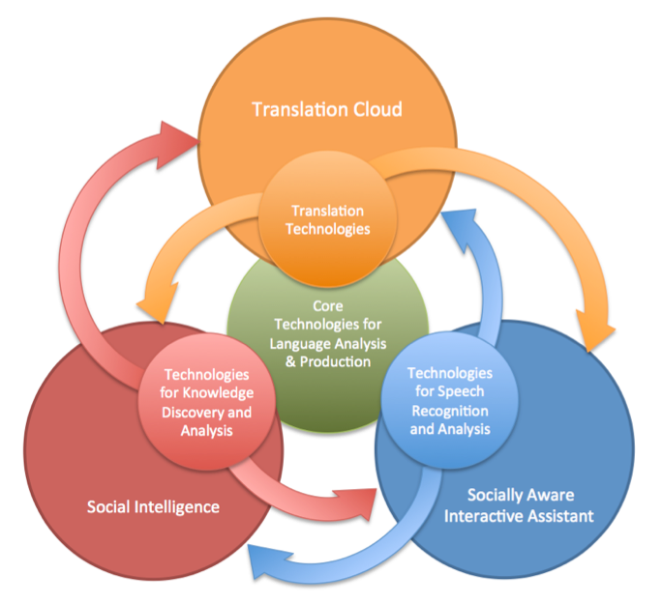
\includegraphics[width=0.75\textwidth]{../_media/PT-Rings}
  \caption{Scientific cooperation among the three priority research themes}
  \label{fig:priority-themes}
  \colorrule{grey3}{\textwidth}{1.5pt}
\end{figure*}
 
All three themes need to benefit from progress in core technologies of language analysis and production such as morphological, syntactic and semantic parsing and generation. But each of the three areas will concentrate on one central area of language technology: the Translation Cloud will focus on cross-lingual technologies such as translation and interpretation; the Social Intelligence strand will take care of knowledge discovery, text analytics and related technologies; the research dedicated to the Interactive Assistant will take on technologies such as speech and multimodal interfaces (see Figure~\ref{fig:priority-themes}).

Except for a few large national projects and programmes such as Technolangue and Quaero in France, Verbmobil and Theseus in Germany and DARPA Communicator and GALE in the US the field of language technology does not have experience with research efforts of the magnitude and scope required for the targeted advances and plans in this SRA. Nevertheless, our technology area has to follow developments in other key engineering disciplines and speed up technology evolution by massive collaboration based on competitive division of labour and sharing of resources and results. In our reflection on optimal schemes for organizing we tried to draw lessons from our own field's recent history and to capitalise on experience from other fields by adopting approaches that proved successful and evading encountered pitfalls.
 
The final model for the organisation of collaboration will have to be guided by a thoughtful combination of the following basic approaches.

% FIXME: cite? http://cacm.acm.org/magazines/2012/7/151226-googles-hybrid-approach-to-research/fulltext

\textbf{Flexible collaborative approach:} For each priority theme, one or several very large cooperating and competing lead projects will share an infrastructure for evaluation, resources (data and base technologies), and communication. Mechanisms for reducing or terminating partner involvements and for adding new partners or subcontracted contributors should provide flexibility. A number of smaller projects including some national and regional projects will provide building blocks for particular languages, tasks, component technologies or resources. A cooperation scheme will be designed for effectively involving EC-funding, contributions from member states, industrial associations, and language communities. The choice of funding instruments will be determined in due time after.

\textbf{Staged approach:} Two major phases are foreseen (2015-2017, 2018-2020). For better concertation the major phases should be synchronised among the themes and also projects.   

\textbf{Evolutionary approach:} Instead of banking on one selected paradigm, competing approaches will be followed in parallel with shared schemes for evaluation, merging, adopting and discontinuing research threads so that the two elements of successful evolutionary research approaches, selection and cross-fertilisation, are exploited to the maximum extent possible.

\textbf{Analytical approach:} Instead of the currently predominant search for an ideal one-fits-all approach, the research will focus on observed quality barriers and not shun computationally expensive dedicated solutions for overcoming particular obstacles.

\textbf{Bootstrapping approach:} Better systems can be derived from more and better data and through new insights. In turn, improved systems can be used to gain better data and new insights. Thus the combination of the analytical evolutionary approach with powerful machine learning techniques will be the basis for a technology bootstrapping, which has been the by far most fruitful scheme for the development of highly complex technologies.

\textbf{Close cooperation with relevant areas of service and technology industries:} In order to increase chances of successful commercialisation and to obtain convincing and sufficiently tested demonstrations of novel applications, the relevant industrial sectors of industry must be strongly integrated into the entire research cycle.

\textbf{Tighter research-innovation cycle:} Through the collaboration between research, commercial services and commercial technology industries, especially through the shared evaluation metrics and continuous testing, the usual push-model of technology transfer will hopefully be substituted by a pull-model, in which commercial technology users can ask for specific solutions. In the envisaged research scheme incentives will be created for competing teams each composed of researchers, commercial users and commercial developers by the participating enterprises for initiating successful innovations.

\textbf{Interdisciplinary approach:} A number of science, technology and service areas need to be integrated into the research from day one. Some technology areas such as speech technologies, language checking and authoring systems need to be represented by providers of state-of-the-art commercial products.

Supporting research and innovation in language technology should be accompanied by policy making in the area of multilingualism, but also in digital accessibility. Overcoming language barriers can greatly influence the future of the EU. Solutions for better communication and for access to content in the native languages of the users would reaffirm the role of the EC to serve the needs of the EU citizens. A substantial connection to the infrastructural program CEF could help to speed up the transfer of research results to badly needed services for the European economy and public.
 
At the same time, use cases should cover areas where the European societal needs massively overlap with business opportunities to achieve funding investment that pays back, ideally public-private partnerships.
 
The coordination among the three research strands poses administrative challenges. Because of the described interdependencies and also because of the need to maintain and improve the obtained level of cohesion and community spirit in the European Language Technology community, a coordinating body is needed. Whether such an entity is jointly carried by the three areas or by a separate support project, needs to be determined in the upcoming discussion on the appropriate support instruments for the identified research priorities.

\subsection{Core Language Resources and Technologies}
\label{sec:sharing-resources-and-results}

% This section is based on Stelios' input (sent on June 29, 2012)

The three priority research themes share a large and heterogeneous group of core technologies for language analysis and production that provide development support through basic modules and datasets (see Figure~\ref{fig:priority-themes}, p.~\pageref{fig:priority-themes}). To this group belong tools and technologies such as, among others, tokenisers, part-of-speech taggers, syntactic parsers, tools for building language models, information retrieval tools, machine learning toolkits, speech recognition and speech synthesis engines, and integrated architectures such as GATE and UIMA. Many of these tools depend on specific datasets (i.\,e., language resources), for example, very large collections of linguistically annotated documents (monolingual or multilingual, aligned corpora), treebanks, grammars, lexicons, thesauri, ontologies and language models. Both the basic tools and especially language resources can be rather general or highly task- or domain-specific, available for free or for a fee, tools can be language-independent, datasets are, by definition, language-specific. As complements to the core technologies and resources there are several types of resources, such as error-annotated corpora for machine translation or spoken dialogue corpora, that are specific to one or more of the three priority themes.

A key component of the suggested research agenda is to collect, develop and make available core technologies and resources through a shared infrastructure so that the research and technology development carried out in all themes can make use of them. Over time, this approach will improve the core technologies, as the specific research will have certain requirements on the software, extending its feature set, performance, accuracy etc.~through dynamic push-pull effetcs. Conceptualising these technologies as a set of shared core technologies will also have positive effects on their sustainability and interoperability.

The European academic and industrial technology community is fully aware of the need for sharing resources such as language data (e.\,g., corpora), language descriptions (e.\,g., lexicons, thesauri, grammars), tools (e.\,g., taggers, stemmers, tokenisers) and core technology components (e.\,g., morphological, syntactic, semantic processing) as a basis for the successful development and implementation of the priority themes. Initiatives such as FLaReNet \cite{flarenetsra2011} and CLARIN have prepared the ground for a culture of sharing, META-NET's open resource exchange infrastructure, META-SHARE, is providing the technological platform as well as legal and organisational schemes. It is also important to note that many European languages other than English are heavily under-resourced, i.\,e., there are no or almost no resources or basic technologies available \cite{LWP2012}.

All language resources and basic technologies that are created under the core technologies umbrella will be shared and made available through the respective infrastructure. The effort should revolve around the following axes: Infrastructure; Coverage, Quality, Adequacy; Language Resources Acquisition; Openness; Interoperability.

% FIXME: Focus upon Knowledge Representation, Semantic Web, Open Data, Linked Open Data, Inferences, Automatic Reasoning etc. a lot more! We have to work together closely with the Semantic Web and W3C people. Named entity recognition and mapping strings to concepts and also attributes to concept features is super important for all three priority research themes.

% FIXME: We have to make sure, especially on the European level, that all (ALL!) languages have a certain set of base technologies and data sets available. Gil F. dazu: 
%
% In modern NLP, everything is based on corpora. When I say "everything" this includes algorithms, annotations, lexica, best practices and so on. But, do we have a corpus representing each European language? The answer is no.
%
% In our 23 official European languages, we have a national corpus for British, Polish, Czech, Slovenian and Bulgarian, that's it. The German reference corpus is badly unbalanced. In French, we have a lot of data but nothing balanced, labelled and maintained, ditto for Spanish.
%
% I think we should organize a corpus for each language with the following properties:
% * balanced genres (e.g. social networks material, newspapers, institutional, technical),
% * balanced modalities (e.g speech, written),
% * open source and free for research and production, for private and public actors.
%
% PS: Take a look at the Open American National Corpus.
%
% FIXME: A comment from Maxim Stamenov.
%
% Development of unified e-dictionaries that are representative of the life and cultural background of each of EU languages – with massive textual and databases support on different lines. Such integrated systems, structured in comparable format and linked multilingually would be, as a matter of fact, a prerequisite for the development on a full-scale of the Translation Cloud. The mapping of such dictionaries (including  the implied diversity of the cultural background of each of them) with their textual support pairwise 23x22 for the 23 official languages of the EU already is a very hard challenge.
%
% [This is not only about technology development, we also need to do a lot of basic research, especially new approaches!] Semantically based knowledge search and representation as a problem requiring new approaches to semantics of natural language and pragmatics of human communication.

\subsubsection{Infrastructure}
\label{sec:infrastructure}

It is imperative to maintain and further to develop META-SHARE. Broad participation by the whole language technology community is essential in maintaining and extending the infrastructure so that acceptance is ensured. META-SHARE will be the key instrument to make language resources available, visible and accessible, to facilitate sharing and exchange of resources.

Among the important aspects that need to be taken care of when taking the next evolutionary steps of the META-SHARE infrastructure are the following: definition of the basic data and software resources that should populate META-SHARE, multilingual coverage, the capacity to attract providers of useful resources, improvements in sharing mechanisms, and collaborative working practices between R\&D and commercial users. There must also be a business-friendly framework to stimulate the commercial use of resources, based on a sound licensing facility. Close cooperation with the three priority themes is of vital importance, especially for defining the set of needed core technologies and resources.

The content of META-SHARE is not limited to data. Instead, it has to be seen as an international hub of resources and technologies for speech and language services from industries and communities. The development and proposal of ideally free tools and, more generally, web services, including evaluation protocols and collaborative workbenches is deemed essential. The accumulation and sharing of resources and tools in a single place would lower the R\&D costs for new applications in new language resource domains.

Sustainability covers preservation, accessibility, and operability (among other things). Collecting and preserving knowledge in the form of existing resources should be a key priority. A sustainability analysis must be part of a resource specification phase, and it is important that funding agencies impose a sustainability plan mandatory for those projects that are concerned with the production of language resources.

Accurate and reliable documentation of resources is an undisputable need. An effort must be made to collect all existing documentations and to make them available as a repository of specifications, guidelines, and documentation of resources. Documentation is also the gateway to resource discovery. Ensuring that resources are discoverable is the first step towards promoting the data economy. 

\subsubsection{Coverage, Quality, Adequacy}
\label{sec:cover-qual-adeq}

With regard to the data-driven paradigm, innovation in LT nowadays crucially depends on language resources. Despite the vast amount of academic and industrial investment, there are not enough available resources to satisfy the needs of all languages, quantitatively and qualitatively. Language resources should be produced and made available for every language, every register, every domain to guarantee full coverage, high quality and adequacy for various applications. New methods of resource development can be exploited to achieve better coverage, for instance shared or distributed ones. It is important to assess the availability of existing resources with respect to their adequacy to applications and technology requirements. This involves assessing the maturity of the technologies for which new resources should be developed. Specifically for the advancement of LTs, basic language resource kits should be supported and developed for all languages and, at least, key applications.

To reduce the amount of human intervention and revision, automatic techniques should be promoted to guarantee quality through error detection and confidence assessment. The promotion of validation and evaluation can play a valuable role in fostering quality improvement. Evaluation should encompass technologies, resources, guidelines and documentation. But like the technologies it addresses, evaluation is constantly evolving, and new, more specific measures using innovative methodologies are needed to evaluate the reliability of language resources, while maximal use of existing tools should be ensured for the validation of resources.

Specific lists of basic language technologies should be compiled that should be either made available or researched and implemented for all languages covered by this document. These should include tools such as sentence boundary detection modules, tokenisers, lemmatizers, taggers, parsers, word/phrase aligners etc.~as obligatory processing components for each language. These should also include lists of basic resources needed for making the modules work for a specific language. Other important aspects are quality thresholds (minimal level of accuracy, speed, open availability, interoperability etc.) and cross-lingual evaluation campaigns organised on a regular basis. There have been partial attempts at these in the past (e.\,g., BLARK and ELARK, shared tasks such as CLEF, EuroMatrix Marathons, IWSLT, Morpho-Olympics etc.) but a more coordinated, sustainable and also wider attempt is needed. 

A “Language Resources Impact Factor (LRIF)” should be defined in order to enforce the practice of citation of resources on the model of scientific paper authoring and to calculate the actual research impact of resources.  A reference model for creating resources will help address the current shortage of resources in terms of breadth (languages and applications) and depth (quality and volume).

\subsubsection{Language Resources Acquisition}
\label{sec:lang-reso-acqu}

Re-use and re-purposing should be encouraged to ensure the reuse of development methods and existing tools. With production costs constantly increasing, there is a need to invest in innovative production methods that involve automatic procedures, so as to reduce human intervention to a minimum. The coverage problem is so enormous that strategies that approach or ensure full automation for high-quality resource production should be promoted. It is worth considering the power of social media to build resources, especially for those languages where there are no language resources built by experts yet.

There are several promising experiments in crowd-sourcing data collection tasks. Crowd-sourcing makes it possible to mobilise large groups of human talent around the world with just the right language skills so that we can collect what we need when we need it. For instance, it has been estimated that Mechanical Turk translation is 10 to 60 times less expensive than professional translation. 

A particularly sensitive case is that of less-resourced languages, where language technology should be developed rapidly to help minority-language speakers access education and the Information Society \cite{eldia12}. Basic language resources for all the world’s languages could be created building a Web 2.0 site starting with the 446 languages currently present on the web. Collaborative and Web 2.0 methods for data collection and annotation seem particularly very well-suited for collecting the data needed for the development of LT applications.

\subsubsection{Openness}
\label{sec:openness}

There is a strong trend towards open data, i.\,e., data that are easily obtainable and that can be used with few, if any, restrictions. Sharing resources (both data and tools) has become a viable solution towards encouraging open data, and the community is strongly investing in facilities such as META-SHARE for the discovery and use of resources. These facilities could represent an optimal intermediate solution to respond to the needs for data variety, ease of retrieval, better data description and community-wide access, while at the same time assisting in clearing the intricate issues associated with intellectual property rights.

The challenge for the community and policy makers is to push for the development of a common legal framework that would facilitate resource sharing efforts abiding by the law, benefiting from the adoption of “fair use” principles and appropriate copyright exceptions. It is of utmost importance that legislation regarding resource use be harmonised, and even standardised, for all types of resources, and that free use be allowed, at least for research or non-profit purposes. 

% FIXME: Mention the META-NET Data Liberation Campaign that we carry out.

% Licensing schemes need to be simplified through broad-based solutions for both R\&D and industry. Electronic licensing (e-licenses) should be adopted and current distribution models to new media (web, mobile devices, etc.) should be accepted.

\subsubsection{Interoperability}
\label{sec:interoperability}

Interoperability of resources seeks to maximise the extent to which they are compatible and therefore integratable at various levels, so as to allow, for instance, the merging of data or tools coming from different sources. % Interoperability is also an essential prerequisite for successful exploitation of the enormous amount of data that the advent of the internet has been making available since less than two decades.
The community and the funding agencies need to join forces to drive forward the use of existing and emerging standards, at least in the areas where there is some degree of consensus. The only way to ensure useful feedback to improve and advance is to use standards on a regular basis. It will be thus even more important to enforce and promote the use of standards at all stages.

\begin{figure*}[htbp]
  \centering
  \small
  \begin{tabular}{@{}p{2.5cm}p{8cm}p{4cm}@{}} \toprule\addlinespace
    \multicolumn{1}{c}{Research Priority} & \multicolumn{1}{c}{Phase 1: 2013-2014} & \multicolumn{1}{c}{Phases 2 and 3: 2015-2020} \\ \addlinespace\midrule\addlinespace
    Infrastructure & Maintain and extend facility(-ies) for sharing resource data and tools; promote accurate and reliable documentation of resources through metadata; cooperation between infrastructure initiatives to avoid the duplication of effort & Create mechanisms for accumulating descriptions of as well as actual resources; multilingual coverage, ease of conversion into uniform formats; solutions for integrating language processing services to help growth of infrastructures (SaaS) \\ \addlinespace
    Coverage, quality, adequacy & Increase quantity of resources available to address language technology and application needs; address formal and content quality of resources by promoting evaluation and validation; promote evaluation and validation activities of resources and the dissemination of their outcomes & Further increase quantity of resources available to address language and application needs; provide high quality resources for all European languages \\ \addlinespace
    Acquisition & Ensure public and community support to definition and dissemination of resource production best practices; enforce reusing and repurposing; research work towards the full automation of LR data production; invest in methods for collaborative creation and extension of high-quality resources, also as a means to achieve better coverage; implement workflows of language processing services for acquisition of resources required for the implementation of the priority themes; bridge acquisition methods with linked open data and big data; share the effort for production of LRs between international bodies and individual countries & \\ \addlinespace
    Openness & Educate key players with basic legal know-how; elaborate specific, simple and harmonised licensing solutions for data resources; promote copyright exception for research purposes; develop legal and technical solutions for privacy protection; opt for openness of resources, especially publicly funded ones;
ensure that publicly funded resources are publicly available free of charge; clear IPR at the early stages of production; try to ensure that re-use is permitted & \\ \addlinespace
    Interoperability & Invest in standardisation activities, make standards operational and put them in use; create permanent Standards Observatory or Standards Watch; promote and disseminate standards to students and young researchers; encourage/enforce use of best practices or standards in production projects; identify new mature areas for standardisation and promote joint efforts between R\&D and industry & \\ \addlinespace\bottomrule
  \end{tabular}
  \caption{Core language resources and technologies: Preliminary Roadmap}
  \label{fig:lrlt-roadmap}
\end{figure*}

\subsubsection{Organisation of Research}
\label{sec:org-research-pt4}

In order to optimise the efficiency of shared core technologies for language analysis and production as well as the further development of the infrastructure, maximise the infrastructure's impact, and ensure that requirements for research and development are met at the necessary depth for all languages in all priority themes, the organisation of this shared component of the research agenda should adopt the following principles: It is necessary to invest in the further development of an integrated infrastructure (i.\,e., META-SHARE) based on an open architecture, enabling the sharing and further development of resources. The infrastructure should support technology-specific challenges and shared tasks in order to accelerate innovation breakthrough and market-readiness for desperately needed technologies. Concerted activities and policies facilitating the sharing of resources overcoming all stumbling blocks on the way to technical, organisational and legal interoperability should be supported. EU level research must be aligned and tightly coordinated with efforts on the national levels, so that language coverage and language-specific developments are efficiently achieved. An important aspect of this coordination effort is concerned with the results of the META-NET White Paper Series: in the 30 different white papers we have concrete and specific assessments of the language- and country-specific situation with regard to demands and technology gaps. The next step is to address and to fill these gaps with high-quality and robust core technologies and language resources. In addition we will continue to collect relevant technologies and resources for inclusion in and distribution through META-SHARE.

% FIXME. Peter Spyns: "tightly coordinated -- but by whom? National funders are very reluctant to leave this to the EC (cf. the current discussions on Horizon 2020 PCs) and the researchers/companies themselves should not do this alone either."

% FIXME: Two remarks from Jürgen Wedekind:
%
% Is it realistic to assume that the required semantic, pragmatic, multimodal, and reasoning "tools and resources" can be developed within 8 years, in particular, if hybrid approaches will be employed. Rule-based approaches are even more costly and time-consuming than statistical approaches. Is the idea to develop them for all European languages? That is even less realistic.
%
%
% It is not entirely clear how the core technologies (language analysis and production) are developed: independently of the priority themes or not? Moreover, the priority themes are very sophisticated and complex in the sense that they depend on many core technologies that also depend or build on each other. This might cause extremely high risk to the completion of the projects of the priority themes.

%\begin{itemize}
%\item This platform should enable resources, data and processing services to be incorporated in, or called by a wide range of application software.
%\item To boost the automation of the language resource acquisition process, thus increasing coverage, quality and adequacy, a small number of coordinating projects attached to a federation of strategic projects with complementary goals can be foreseen. These projects should be objective-driven, with clear research, technology and exploitation milestones, coordinated by an ongoing road-mapping effort.
%\item In order to increase research efficiency within a public-private partnership, the preferred infrastructure should handle the various applications in connection with the cooperative development of technologies, including regular objective evaluation of technology progress, and the production of the appropriate resources which are necessary to develop and test the various technologies.
%\end{itemize}

% ------- End of Stelios' text

\subsection{Challenges for Innovation}
\label{sec:powerf-mech-showcasing-and-innovation}

% FIXME: Isn't this section now obsolete if we say that the section on Market Opportunities and Innovation will be provided by LT Innovate? Rather say nothing than have a short and rather vague section such as this one?

Language Technology is innovation-friendly in the sense that many solutions are not standardised, but require individual adaptation or new development for a certain customer or application. Thus, one can truly speak of socially responsible innovation here.

As there are many niches in the market that are not targeted by the big players, SMEs have real opportunities. At the same time, language technology, as a key-enabling technology, usually enters the markets in combination with other technologies as an essential component of novel products and services that can be arbitrarily complex, which has made it difficult for SMEs to identify customers in the past.

The question is how to transform innovation and research into new products, markets, growth, and, finally, new jobs. In recent years, drivers for innovations have often been applications and tools such as Skype, Facebook, or recommender systems that have been designed by smaller teams and start-ups. Important aspects of their success stories, besides the core and novel functionalities and feature sets for which there was an obvious need, often was their fast and viral outreach and uptake through social networks. 

Large global platforms for novel end-user-services have also become the predominant innovation drivers for language technology solutions. These platforms can be web services such as Google Search that integrates the new Knowledge Graph concept network, speech-enabled search \cite{meisel12} and also web translation. Combinations of hardware and operating systems such as iOS for Apple's mobile devices can also be considered platforms. Or it could be an open operating system such as Android which recently extended its current speech and language functionalities with a mobile assistant.

The trend towards widely used platforms will drastically facilitate the spreading of innovative language technologies. Actually, language technology has a good chance of becoming the essential feature for the success of the next generation of services. At closer inspection, the integration of sophisticated language technology in current platforms is rather limited, scratching only the surface of what will be possible in the near future.

Apart from new ways of sharing, development, and distribution, a generally innovative climate is needed. The availability of venture capital and meeting points such as summits where research and decision makers from industry get together should be backed by public funding and uptake. Flexibly funded consortia that run over a longer period with changing partners, where research and innovation phases lead over to product development and marketing would also support innovation. Research centres and companies that develop highly innovative approaches or technologies should get incentives, for example, bonus grants, awards or prizes. In addition we have to bring the language technology landscape and the European startup scene together in order to foster innovation between these two communities that only very partially overlap.

In META-NET we tried to bring together the largely fragmented European Language Technology technology. It is of utmost importance that this community building aspect is continued and further strengthened in order to enable companies to cooperate and to being competitive, especially with regard to the shared European programme that we plan. 

Another aspect on a more abstract but also crucial level is the existence of the English language innovation bias: the discourse on innovation has become determined by the English language, and the media reporting in that language. As Mark Vanderbeeken, a Belgian who lives in Italy notes in a widely read essay \cite{vanderbeeken2012}, this sheer dominance of English carries with it an accompanying perspective of Europe, both in terms of stereotypes and in terms of relevance to the Anglo-Saxon world. In turn, this puts European businesses and countries at a serious disadvantage that they are not aware of. But it also disadvantages businesses in the English-speaking world, which are perhaps not aware that they are receiving an abbreviated picture of innovation in Europe. This is a phenomenon that Vanderbeeken terms ``the non-English disadvantage''. This is another example of a disadvantage which can be successfully addressed, especially on the European level, through multilingual technologies.

%\subsection{A European Service Platform for Language Understanding, Communication, Knowledge, Inference and Emotion}

\subsection{A European Service Platform for Language Technologies}
\label{sec:europ-service-platform}

% Possible Names and Acronyms for the Platform:
%
% EuroLang:   European Language(s) Platform
% PEL:        Platform for European Languages
% PELT:       Platform for European Language Technology
% CompCom:    Computers and Communication
% LUCKIE SKY: Platform for Language Understanding, Communication, Knowledge, Inference and Emotion

We argue for the creation of an ambitious large-scale sky-computing platform as a central motor for research and innovation in the next phase of IT evolution and a ubiquitous resource for the multilingual European society (an idea suggested by several experts from industry in META-NET Vision Group meetings). The platform will be used for testing, show casing, proof-of-concept demonstration, avant-garde adoption, experimental and operational service composition, and fast and economical service delivery to enterprises and end-users.
 
The proposed creation of a powerful cloud or sky computing platform (see Section~\ref{sec:cloud-sky-computing}) for a wide range of services dealing with human language, knowledge and emotion will not only benefit the individual and corporate users of these technologies but also the providers.
 
\textbf{Users} will be able to receive customised integrated services without having to install, combine, support and maintain the software. They will have access to specialised solutions even if they do not use these regularly.
 
\textbf{Language technology providers} will have ample opportunity to offer services stand-alone or integrated with others.
 
\textbf{Providers of language services} rendered by human language professionals will be able to use the platform for enhancing their services by means of appropriate technology and for providing their services stand-alone or integrated into other application services.
 
\textbf{Researchers} will have a unique virtual laboratory for testing, combining, and benchmarking their novel technologies and for exposing them in realistic trials to real tasks and end users.
 
\textbf{Providers of services} that can be enabled or enhanced by text and speech processing will utilise the platform for testing the needed LT functionalities and for integrating them into their own solutions.

\textbf{Citizens and corporate users} will enjoy the benefits of language technology early and at no or reasonable costs through a large variety of generic and specialised services offered at a single source.

In order to allow for the gigantic range of foreseeable and currently not yet foreseeable solutions, the infrastructure will have to host all relevant simple services, including components, tools and data resources, as well as various layers or components of higher services that incorporate simpler ones. This is why META-SHARE will play an important role in the design of the overall platform (see section~\ref{sec:sharing-resources-and-results}).
 
A top layer consists of \textbf{language processing} such as text filters, tokenisation, spell checking, grammar checking, style checking, hyphenation, lemmatising and parsing. At a slightly deeper level, services will be offered that realise some degree and form of \textbf{language understanding} including entity and event extraction, opinion mining and translation. Both basic language processing and understanding will be used by services that support \textbf{human communication} or realise some human-machine interaction. Part of this layer are question answering and dialogue systems as well as email response applications. Another component will bring in services for processing and storing \textbf{knowledge} gained by and used for understanding and communication. This part will include repositories of linked data and ontologies, as well as services for building, using and maintaining them. These in turn permit a certain range of rational capabilities often attributed to a notion of intelligence. The goal is not to model the entire human intelligence but rather to realise selected forms of \textbf{inference} that are needed for utilising and extending knowledge, for understanding and for successful communication. These forms of inference permit better decision support, pro-active planning and autonomous adaptation. A final part of services will be dedicated to \textbf{human emotion}. Since people are largely guided by their emotions and strongly affected by the emotions of others, truly user-centred IT need facilities for detecting and interpreting emotion and even for expressing emotional states in communication. 

We consider the paradigm of federated cloud services or sky computing with its emerging standards such as OCCI, OVM and CDMI and toolkits such a OpenNebula as the appropriate approach for realising the ambitious infrastructure. All three priority areas of this SRA will be able to contribute to and at the same time draw immense benefits from this platform. There are strong reasons for aiming at a single service platform for the three areas and for the different types of technologies. They share many basic components and they need to be combined for many valuable applications, including the selected showcase solution of the three areas.

% Because of its components (language, understanding, communi­cation, knowledge, inference and emotion) we subsume the entire set of services under the acronym LUCKIE.  
 
\subsubsection{Implementation of the Platform}
\label{sec:implementation-of-platform}

The creation of the platform, for which a name has yet to be found, has to be supported by public funding. Because of the high requirements concerning performance, reliability, user support, scalability, persistence as well as data protection and conformance with privacy regulation, the platform needs to be established by a consortium with strong commercial partners and also be operated by this consortium or a commercial contractor. A similar platform with slightly different desiderata and functionalities is currently built under the name Helix-Nebula for the Earth Sciences with the help of the following commercial partners: Atos, Capgemini, CloudSigma, Interoute, Logica, Orange Business Services, SAP, SixSq, Telefonica, Terradue, Thales, The Server Labs and T-Systems. Partners are also the Cloud Security Alliance, the OpenNebula Project and the European Grid Infrastructure. These are working together with major research centres in the earth sciences to establish the targeted federated and secure high-performance computing cloud platform.
 
The intended platform for LT and neighbouring fields would be intended for a mix of commercial and non-commercial services. It would be cost-free for all providers of non-commercial services (cost-free and advertisement-free) including research systems, experimental services and freely shared resources but it would raise revenues by charging a proportional commission on all commercially provided services. In order to reduce dependence on individual companies and software products, the base technology should be supplied by open toolkits and standards such as OpenNebula and OCCI.  
 
For each priority research theme, chances for successful showcasing and successful commercial innovation will increase tremendously if usable services could be offered on such a platform of required strength and reliability.
 
The platform will considerably lower the barrier for market entry for innovative technologies, especially for products and services offered by SMEs. Still, these stakeholders may not have the resources, expertise, and time to create the necessary interfaces to integrate their results into real-life services, let alone the overarching platform itself. There is still a gap between research prototypes and products that have been engineered and tested for robust applications. Moreover, many innovative developments require access to special kind of language resources such as recordings of spoken commands to smartphones, which are difficult to get for several reasons.
 
Thus the service platform will be an important instrument for supporting the entire innovation chain, but, in addition, interoperability standards, interfacing tools, middle-ware, and reference service architectures need to be developed and constantly adapted. Many of these may not be generic enough to serve all application areas, so that much of the work in resource service integration will have to take place in the respective priority theme research actions.

\subsubsection{Legal Aspects}
\label{sec:legal-aspects}

% FIXME: Important comments from Serge Gladkoff that can probably best be integrated here.
%
% % Looking into the issues of privacy, IP, patented and proprietary technologies
% While reading the SRA many questions arise on various legal aspects of future research and development efforts:
% 1)	It is reasonable to believe that not all of technologies will developed from scratch; existing technologies will be used (algorithms, software code, software packages and systems, architecture of computational networks and databases, as well as protocols and data formats). It is therefore inevitable that copyright issues and licensing issues will arise. This aspect does not seem to be fully covered in the Agenda. Even if everything will be developed from scratch, there are patented technologies that prevent using the ideas that have been already appropriated.
% 2)	It is also necessary to look for other important legal aspects of the future “centralized”, “cloud” model of services, data and knowledge. The SRA is planning to digitize, put into the Cloud and open access to the lot of information. It is therefore worth thinking about how legitimate this is going to be. Many issues may arise, such as copyrighted content, protection of confidential information and fighting crimes in cyberspace.
% 3)	Personal, private information protection requires special attention. For example, assistance in translating patient data may require additional measures to protect personal information;
% 4)	Content which is not appropriate or even legal in one country may be within the limits on another; translation therefore must take into account legal realms.
% 5)	Commercial, proprietary information, national and international security must also be protected with special measures;
% 6)	E-democracy, social intelligence and participation has also another side of the coin – negative and even criminal communities and groups should be in check and the balance is therefore required between freedom of speech and privacy and the need to be able to identify all the authors of potentially harmful content. Authors must be identified and in multilingual Europe translators, editors and reviewers must also be in some cases identified to ensure proper responsibility allocation.
% 7)	It is not yet quite the digital world; many documents are still processed in paper form. Documents still travel paper routes and change in the process, with comments, additions and revisions. The problem of synchronization of paper and digital content is key to integration of paper and digital worlds.
% 8)	Consequently, a “service” research theme must be envisaged to foresee 
% SUGGESTION: Recognize these hurdles of digital multilingual future in SRA, so as to provision the funds and research to cope with these challenges of the future and develop the program properly.

\end{multicols}

% --------------------------------------------------------------------------

\clearpage

\ssection[Towards Roadmaps and a Shared European Programme for Multilingual Europe 2020]{Towards Roadmaps and a\newline Shared European Programme for\newline Multilingual Europe 2020}
\label{sec:conclusions}

% FIXME: This chapter needs to be seriously revised!

\begin{multicols}{2}
\subsection{Improved Education and Training}
\label{sec:improved-edu-and-training}

An indispensable prerequisite for innovative research and technology development are highly qualified researchers and software developers. In the ca.~two years it took us to prepare what is now contained in this strategic research agenda, we talked to representatives of many companies. Almost without exception these industry representatives mentioned the lack of qualified personnel to be a significiant problem for their further growth and diminishing factor as regards producing highly innovative technologies. Europe's academic programmes in Natural Language Processing, Computational Linguistics, Language Technologies, Language-Oriented Information Processing etc.~need to be further strengthened and advertised on a European level and especially made more attractive for potential students. In a later implementation phase of our Strategic Research Agenda we also need to introduce coordinated training programmes for IT professionals and software developers who are not yet familiar with language technologies so that they are made aware of our tools, resources and technologies and learn how to make use of them in their own IT landscapes. The lack of skilled personnel --~from students to senior software engineers~-- currently is a, if not \emph{the} major bottleneck for many small and medium companies and also research centres. In addition, future users of language technologies need to be equipped with at least some background in general linguistics, computational linguistics, natural language processing, speech and related basic technologies.

\subsection{Towards Roadmaps}
\label{sec:roadmaps}

Important components of the final version of this Strategic Research Agenda will be a small set of roadmaps that provide additional details with regard to the actual steps, order, priorities and dependencies of the research foreseen for a total of five areas. In addition to the three priority research themes (Sections~\ref{sec:priority-theme-1-translation-cloud}, \ref{sec:priority-theme-2-social-intelligence} and~\ref{sec:priority-theme-3-interactive-assistant}), roadmaps have to be prepared for the core language technologies and shared resources area (Section~\ref{sec:sharing-resources-and-results}) and the European service platform for language technologies (Section~\ref{sec:europ-service-platform}).

\subsection{Towards A Shared European Programme}
\label{sec:towards-shar-europ}

The plans foreseen in this SRA can be successfully realised and implemented using a number of different measures and instruments, for example, through clusters of projects or a certain number of coordinated projects. Also an option is to set up a shared programme between the European Commission and the Member States as well as Associated Countries. First steps along those lines have been taken at META-NET's META-FORUM 2012 conference in Brussels, Belgium, on June 21, 2012, when representatives of several European funding agencies who participated in a panel discussion on this topic, unanimously expressed the urgent need for such a shared programme.

A sizable portion of the research proposed in this SRA under the umbrella of the three priority themes is to be carried out in the Horizon 2020 programme. The European service platform for language technologies is a very good fit for the Connecting Europe Facility programme (CEF) while large parts of the core technologies for language analysis and production are good candidates for support through national and regional programmes.

There are several options how to organise the research proposed in this strategic agenda. In June 2012 we have started discussing two possible instruments within META-NET that mainly aim at establishing a shared European programme -- several other options still have to be screened. The two candidate instruments are an Article 185 Initiative (see Section~\ref{sec:article-185-init}) and a Contractual Public-Private Partnership (PPP, see Section~\ref{sec:contr-ppp}).

% FIXME: Very good remark from Peter Spyns:
%
% "In order to convince national funders to participate, you’ll have to very carefully sketch a governance structure that performs the checks and balances and monitors the progress.  The short sections in chapter 7 are not really convincing yet. And the big question will be about the coordination and the decisions on which paths to follow and which no more (who decides, according to which criteria etc.). The report does not set quality levels: e.g. translation in the cloud – but not level of translation quality. Organising evaluation tracks will (or rather must) be a major quality insurance instrument, otherwise we end up (once again) with research prototypes that do not comply with industry expectations or performance standards. So strong involvement of industry is a must."

% FIXME: Remark from Koenraad De Smedt: 
%
% With respect to funding mechanisms, the demands of writing project applications and reports are currently so high that they cause prohibitive overhead costs to potential applicants.  Also, it is not obvious for SMEs to get research funding without necessarily being a part of huge networks, even if small creative organizations can move more quickly than big consortia.  These practical bottlenecks need a solution before more European SMEs will effectively take part in R\&D programmes.

\subsubsection{Article 185 Initiative}
\label{sec:article-185-init}

To quote Article 185 of the Treaty of the Functioning of the European Union (TFEU): ``In implementing the multiannual framework programme, the Union may make provision, in agreement with the Member States concerned, for participation in research and development programmes undertaken by several Member States [\dots].''  Currently there are four joint programmes running as Article 185 Initiatives \cite{A185}: Ambient Assisted Living (AAL), Baltic Sea research (Bonus), a programme in the field of metrology (EMRP) and a programme for research performing SMEs and their partners (Eurostars).

A key idea behind Article 185 is to coordinate national programmes in order to reduce the fragmentation of research efforts carried out on the national or regional level. Among the goals to be achieved are to reach critical mass in certain research areas, to ensure better use of scarce resources and to find common answers and approaches to common needs and interests. Member states are given the opportunity to exchange good practice, to avoid unnecessary overlaps of efforts, to exchange information and expertise and to learn from each other.

The Seventh Framework Programme states that an Article 185 Initiative can be launched in areas to be identified in close association with the Member States on the basis of a series of criteria: relevance to EU objectives; the clear definition of the objective to be pursued and its relevance to the objectives of the Framework Programme; presence of a pre-existing basis (existing or envisaged research programmes); European added value; critical mass, with regard to the size and the number of programmes involved and the similarity of activities they cover; efficiency of Article 185 as the most appropriate means for achieving the objectives. Each Article 185 Initiative is set up individually through a decision of the European Parliament and of the European Council, following a proposal from the European Commission.

% The implementation requires the establishment or existence of a legal Dedicated Implementation Structure (DIS) which should exist before the Council's decision. The DIS takes care of programme management and calls for proposals, selection of projects and follow-ups and financial management.

\subsubsection{Contractual Public-Private Partnership}
\label{sec:contr-ppp}

While many details of the upcoming programme Horizon 2020 are still under discussion, Contractual PPPs are currently emerging as the primary model to implement parts of the programme objectives with regard to sizeable, roadmap-based research and innovation efforts within the technology pillar of H2020, drawing also on resources beyond the EU support and related matching funds. The EC's proposal for Horizon 2020 states that ``greater impact should also be achieved by combining Horizon 2020 and private sector funds within public-private partnerships in key areas where research and innovation could contribute to Europe's wider competitiveness goals and help tackle societal challenges'' \cite{H2020prop}.  PPPs are an important mechanism for focusing research and innovation, ensuring stakeholders engagement and, above all, for improving the impact of EU support on Europe's competitiveness, growth and jobs creation. A public-private partnership is defined as ``a partnership where private sector partners, the Union and, where appropriate, other partners, commit to jointly support the development and implementation of a research and innovation programme or activities''. Similar instruments are JTIs (Joint Technology Initiatives), ETPs (European Technology Platforms) and institutional PPPs which are a counterpart to Contractual PPPs.

For Contractual PPPs, a Contractual Agreement is foreseen between the EC and private and public partners that specifies the objectives of the partnership, commitments of the partners, target outputs and the activities that require support from Horizon 2020. PPPs are to be identified in an open and transparent way based on all of the following criteria: the added value of action at Union level; the scale of impact on industrial competitiveness, sustainable growth and socio-economic issues; the long-term commitment from all partners based on a shared vision and clearly defined objectives; the scale of the resources involved and the ability to leverage additional investments in research and innovation; a clear definition of roles for each of the partners and agreed key performance indicators over the period chosen (see \cite{H2020prop}, p.~21).

In contrast to an Article 185 Initiative, setting up a contractual PPP does not require a decision in the European Parliament. This is why a PPP for the priority research themes specified in this Strategic Research Agenda might be a promising avenue.  

\subsubsection{Conclusions}
\label{sec:funding-conclusions}

The research plans specified in this SRA are, among others, a good match for an Article 185 Initiative and also for a Contractual PPP. It remains to be discussed which instrument or maybe even set of carefully selected and compiled instruments is considered the most appropriate one to realise and implement the three priority research themes, the set of core technologies and shared resources and also the European service platform for language technology.

% FIXME: Following are a few good reasons why this SRA should be implemented through a A185I
% Multilingualism is an important topic and a high societal challenge within the EU. By definition, language technology needs major investments as there are substantial amounts of research efforts needed to prepare and create technologies for every language. Industrial coverage by SMEs plays an important role. The member states, associated countries and also regions are interested to support their languages. The European Union is interested to enable their citizens and businesses to communicate with one another. The bodies of the European Union (EC, EP, ECJ, EPO, ENISA etc.) are interested in supporting their own technological needs with regard to communication and multilingual technologies. 

\end{multicols}

\clearpage

% --------------------------------------------------------------------------

\appendix
\addtocontents{toc}{\protect\bigskip}

% ===========================================================================

\ssection[References]{References}
\bibliographystyle{unsrt}
\bibliography{sra_references}

\clearpage

% ===========================================================================

\ssection[List of Key Contributors]{List of Key Contributors}
\label{sec:list-of-contributors}

The experts listed in the following contributed to this Strategic Research Agenda (54\% from Language Technology User or Provider Industries, 46\% from Language Technology Research, 4\% from national or international institutions), which was edited by the \href{http://www.meta-net.eu/vision/technology-council-members/all}{META Technology Council}.

% Gesamt:    190
%
% Industry:  102
% Academia:   87
% Other:       8 (EPO, JRC, Ministry of Defense, France)

\begin{multicols}{3}
\begin{small}
  \begin{enumerate}
    \raggedright{
      \item Sophia Ananiadou, University of Manchester, UK
      \item Sanne Andresen, Ordbogen, Denmark
      \item Toni Badia, Barcelona Media, Spain
      \item Antonio Balvet, University of Lille, France
      \item Michaela Bartelt, Electronic Arts, Germany/USA
      \item Christoph Bauer, ORF, Austria
      \item Matthias Bärwolff, Tazaldoo, Germany
      \item Caterina Berbenni-Rehm, Promis, Luxembourg
      \item Juanjo Bermudez, Lingua e-Solutions SL, Spain
      \item Henriette Edvarda Berntsen, Tansa, Norway
      \item Nozha Boujemaa, INRIA, France
      \item Hervé Bourland, IDIAP, Switzerland
      \item Antonio Branco, University of Lisbon, Portugal
      \item Andrew Bredenkamp, acrolinx, Germany
      \item Anton Bregar, Poland
      \item Gerhard Budin, University of Vienna, Austria
      \item Axel Buendia, Spir.\,Ops, France
      \item Paul Buitelaar, DERI, Ireland
      \item Aljoscha Burchardt, DFKI, Germany
      \item Will Burgett, Intel, USA
      \item Johannes Bursch, Daimler AG, Germany
      \item Miriam Butt, University of Konstanz, Germany
      \item Nicoletta Calzolari, Consiglio Nazionale delle Ricerche, Italy
      \item Nick Campbell, Trinity College Dublin, Ireland
      \item Olga Caprotti, University of Gothenburg, Sweden
      \item Jean Carrive, INA, France
      \item Khalid Choukri, ELDA, France
      \item Philipp Cimiano, University of Bielefeld, Germany
      \item Ann Copestake, University of Cambridge, UK
      \item Ido Dagan, Bar-Ilan University, Israel
      \item Morena Danieli, Loquendo, Italy
      \item Christophe Declercq, Imperial College, UK
      \item Claude de Loupy, Syllabs, France
      \item Maarten de Rijke, University of Amsterdam, The Netherlands
      \item Koenraad De Smedt, University of Bergen, Norway
      \item István Dienes, Hungary
      \item Alice Dijkstra, Nederlandse Organisatie voor Wetenschappelijk Onderzoek, The Netherlands
      \item Marin Dimitrov, Ontotext, Bulgaria
      \item Petar Djekic, SoundCloud, UK
      \item Bill Dolan, Microsoft, USA
      \item Rickard Domeij, Language Council of Sweden, Sweden
      \item Christoph Dosch, Institut für Rundfunktechnik, Germany
      \item Christian Dugast, Tech2Biz, Germany
      \item Ray Fabri, University of Malta, Malta
      \item Marcello Federico, FBK, Italy
      \item David Filip, Moravia, Czech Republic
      \item Dan Flickinger, Stanford University, USA
      \item Gil Francopoulo, CNRS/LIMSI, IMMI, Tagmatica, France
      \item Piotr W.~Fuglewicz, TiP, Poland
      \item Robert Gaizauskas, University of Sheffield, UK
      \item Martine Garnier-Rizet, CNRS/LIMSI and IMMI, France
      \item Simon Garrett, British Telecom, UK
      \item Stefan Geissler, Temis, Germany
      \item Edouard Geoffrois, Ministry of Defense and French National Research Agency, France
      \item Yota Georgakopolou, European Captioning Institute, UK
      \item Jost Gippert, University of Frankfurt, Germany
      \item Mircea Giurgiu, University of Cluj-Napoca, Romania
      \item Serge Gladkoff, Logrus International and GALA Standards Director, USA/Russia
      \item Daniel Grasmick, Lucy Software, Germany
      \item Gregory Grefenstette, Exalead, France
      \item Marko Grobelnik, Institut ``Jožef Stefan'', Slovenia
      \item Joakim Gustafson, KTH Royal Institute of Technology, Sweden
      \item Thomas Hagen, Dictatr AS, Norway
      \item Jan Hajic, Charles University Prague, Czech Republic
      \item Paul Heisterkamp, Daimler AG, Germany
      \item Mattias Heldner, KTH Royal Institute of Technology, Sweden
      \item Sebastian Hellmann, University of Leipzig, Germany
      \item Manuel Herranz, PangeaMT, Spain
      \item Theo Hoffenberg, Softissimo, France
      \item Thomas Hofmann, Google, Switzerland/USA
      \item Timo Honkela, Aalto University, Finland
      \item Roman Jansen-Winkeln, Belingoo Media Group, Luxembourg
      \item Krzysztof Jassem, Poleng, Poland
      \item Keith Jeffery, Science and Technology Facilities Council, Rutherford Appleton Lab., UK
      \item Richard Jelinek, PetaMem GmbH, Germany
      \item Kristiina Jokinen, University of Helsinki, Finland
      \item Rebecca Jonson, Artificial Solutions, Spain
      \item John Judge, Dublin City University and CNGL, Ireland
      \item Martin Kay, Stanford University, USA and Universität des Saarlandes, Germany
      \item Melih Karakulukcu, Karakulukcu Consulting, Turkey
      \item Jussi Karlgren, Gavagai, Finland
      \item Marc Kemps-Snijders, Meertens Instituut, The Netherlands
      \item Ilan Kernerman, K Dictionaries, Israel
      \item Christopher Kermorvant, A2iA, France
      \item Simon King, University of Edinburgh, UK
      \item Philipp Koehn, University of Edinburgh, UK
      \item Maria Koutsombogera, ILSP, Greece
      \item Steven Krauwer, University of Utrecht, The Netherlands
      \item Verena Krawarik, APA, Austria
      \item Stefan Kreckwitz, Across, Germany
      \item Simon Krek, Institut ``Jožef Stefan'', Slovenia
      \item Brigitte Krenn, OFAI, Austria
      \item Sandra Kübler, Indiana University, USA
      \item Michal Küfhaber, Skrivanek, Czech Republic
      \item Serg Kulikov, Russian Academy of Sciences, Russia
      \item Jimmy Kunzmann, EML, Germany
      \item Gunn Inger Lyse Samdal, University of Bergen, Sweden
      \item Bernardo Magnini, FBK, Italy
      \item Gudrun Magnusdottir, ESTeam, Sweden
      \item Elisabeth Maier, CLS Communication, Switzerland
      \item Joseph Mariani, CNRS/LIMSI and IMMI, France
      \item Penny Marinou, Litterae Trans, Greece
      \item Margaretha Mazura, EMF, UK/Belgium
      \item John McNaught, University of Manchester, UK
      \item Erhan Mengusoglu, Mantis, Turkey
      \item Wolfgang Menzel, University of Hamburg, Germany
      \item Roger Moore, University of Sheffield, UK
      \item Sukumar Munshi, Across, Germany
      \item Bart Noe, Jabbla, Belgium
      \item Torbjørn Nordgård, LINGIT AS, Norway
      \item Jan Odijk, University of Utrecht, The Netherlands
      \item Stephan Oepen, University of Oslo, Norway
      \item Karel Oliva, Czech Academy of Sciences, Czech Republic
      \item Mehmed Özkan, Bogazici University, Turkey
      \item Maja Pantic, Imperial College London, UK
      \item Niko Papula, Mutilizer, Finland
      \item Alexandre Passant, DERI, Ireland
      \item Pavel Pecina, Dublin City University and CNGL, Ireland
      \item Manfred Pinkal, Universität des Saarlandes, Germany
      \item Stelios Piperidis, ILSP, Greece
      \item László Podhorányi, Vodafone, Hungary
      \item Jörg Porsiel, VW, Germany
      \item Gabor Proszeky, Morphologic, Hungary
      \item Artur Raczynski, European Patent Office, Germany
      \item Jens Erik Rasmussen, Mikroverkstedet, Norway
      \item Georg Rehm, DFKI, Germany
      \item Steve Renals, University of Edinburgh, UK
      \item Peter Revsbech, Ordbogen, Denmark
      \item Giuseppe Riccardi, University of Trento, Italy
      \item Daniel Ridings, Mikroverkstedet AS, LINGIT AS, Norway
      \item Eirikur Rögnvaldsson, University of Iceland, Iceland
      \item Philippe Rohou, ERCIM, France
      \item Günther Roscher, ICS Dr.~G.~Roscher GmbH, Germany
      \item Johann Roturier, Symantec, Ireland
      \item Dimitris Sabatakakis, Systran, France
      \item David Sadek, Institute Telecom, France
      \item Sergi Sagàs, MediaPro, Spain
      \item Felix Sasaki, W3C and DFKI, Germany
      \item Jana Šatková, ACP Traductera, Czech Republic
      \item Maneerat Sawasdiwat, Rajamangala University of Technology, Thailand
      \item David Schlangen, University of Bielefeld, Germany
      \item Jörg Schütz, Bioloom, Germany
      \item Bjørn Seljebotn, Nynodata, Norway
      \item Max Silberztein, Université de Franche-Comté, France
      \item Mirko Silvestrini, Rapidrad, Italy
      \item Ruud Smeulders, Rabo Bank, The Netherlands
      \item Svetlana Sokolova, ProMT, Russia
      \item Ralf Steinberger, Joint Research Centre, EC, Italy
      \item Juan Manuel Soto, Fonetic, Spain
      \item Lucia Specia, University of Sheffield, UK
      \item C.\,M.~Sperberg-McQueen, BlackMesa Technologies, USA
      \item Peter Spyns, Flemish Government, Belgium
      \item Maxim Stamenov, Bulgarian Academy of Sciences, Bulgaria
      \item Kerstin Steffen, Maravision, Spain
      \item Volker Steinbiss, RWTH Aachen and Accipio, Germany
      \item Rudi Studer, KIT, Germany
      \item Katerina Stuparicova, Charles University Prague, Czech Republic
      \item Daniel Tapias, Sigma Tech, Spain
      \item Alessandro Tescari, Pervoice, Italy
      \item Lori Thicke, Translators without Borders and Lexcelera, France
      \item Gregor Thurmair, Linguatec, Germany
      \item Rudy Tirry, Lionbridge, Belgium
      \item Attila Törcsvári, Arcanum Development, Hungary
      \item Diana Trandabat, University of A.\,I.~Cuza, Romania
      \item Isabel Trancoso, INESC-ID, Portugal
      \item Dan Tufis, Romanian Academy, Romania
      \item Hans Uszkoreit, DFKI and Universität des Saarlandes, Germany
      \item Erik van der Goot, Joint Research Center, EC, Italy
      \item Peggy van der Kreeft, Deutsche Welle, Germany
      \item Jaap van der Meer, TAUS, The Netherlands
      \item René van Erk, Wolters Kluwer, The Netherlands
      \item Josef van Genabith, Dublin City University and CNGL, Ireland
      \item Arjan van Hessen, Twente University and Telecats, The Netherlands
      \item David van Leeuwen, TNO and Radboud University, The Netherlands
      \item Andrejs Vasiljevs, Tilde, Latvia
      \item Michel Vérel, VecSys, France
      \item Kjersti Drøsdal Vikøren, Standard Norge AS, Norway
      \item Bo Vincents, Ankiro, Denmark
      \item Claire Waast, EDF, France
      \item Philippe Wacker, EMF, UK/Belgium
      \item Wolfgang Wahlster, DFKI, Germany
      \item Alex Waibel, KIT, Germany and CMU, Jibbigo, USA
      \item Jürgen Wedekind, University of Copenhagen, Denmark
      \item André Wlodarczyk, University of Charles De Gaulle, France
      \item Feiyu Xu, DFKI, Germany
      \item Annie Zaenen, University of Stanford, USA
      \item Jakub Zavrel, Textkernel, The Netherlands
      \item Patricia Zimmermann, SpeechConcept GmbH, Germany
      \item Elie Znaty, VecSys, France
      \item Chenqing Zong, Chinese Academy of Sciences, China
    }
  \end{enumerate}
\end{small}
\end{multicols}
  
\clearpage

% --------------------------------------------------------------------------

\ssection[About META-NET]{About META-NET}
\label{sec:app-meta-net}

% FIXME: Comment from Serge Gladkoff.
%
% Serge möchte hier natürlich wegen GALA mehr Prominenz für Verbände. Daher einfach hier in diesem Appendix die Mitgliedsbasis von META etwas genauer erläutern und evtl. vollständig auflisten in sehr kleiner Schrift und mit ein paar wichtigen Attributen (Forschung vs. Industrie, Land etc.).
%
%%  Adding language industry to the picture: getting LSPs, Associations, Industry Bodies, initiatives involved
% Modern economy is driven forward by free market. Free market is a “boiling ocean” of commercial entities of all kinds and scale. These entities are active agents of change, and display self-organization. They form industry associations, initiatives, communities, discussions. All these structures and phenomena facilitate further development of the market. Companies work with their industries via associations. Visionary individuals launch initiatives supported by the funding from those convinced. Educational and research institutions create knowledge by teaching students and doing the research. Government bodies must facilitate this “boiling soup” where life is born.
% SRA must not only focus on technology, it should also care for the society and the industries by cooperating with industry bodies, groups and communities. Social communication about the importance of SRA is of essence. With this view in mind, the theme “social intelligence and participation” can and must be used to advance the program and the future itself, that is to be not only the goal, but also the vehicle of the Program.

% SUGGESTION:
% 1.	Amend SRA with the section “Working with the society and the industry: engaging the people who are capable to be agents of change and want to be engaged.”
% 2.	Provision space for communities, groups and Associations in future research agenda and development process. In a way it’s already happening with META Technology Council itself and LT-Innovate Program, but why don’t we make this “official”. Concrete measures, programs and plans must be thought out in order to get all those constituencies properly involved, and it is also a matter of research and trial.

\begin{multicols}{2}
  \textbf{META-NET} is a Network of Excellence partially funded by the European Commission \cite{rehm2011}.  The network currently consists of 60 members in 34 European countries. META-NET forges the Multilingual Europe Technology Alliance (\textbf{META}), a growing community of currently more than 600 language technology professionals and organisations. META-NET fosters the technological foundations for a multilingual European information society that: 1.~makes communication and cooperation possible across languages; 2.~grants all Europeans equal access to information and knowledge regardless of their language; 3.~builds upon and advances functionalities of networked information technology.

The network supports a Europe that unites as a single digital market and information space. It stimulates and promotes multilingual technologies for all European languages. These technologies support automatic translation, content production, information processing and knowledge management for a wide variety of subject domains and applications. They also enable intuitive language-based interfaces to technology ranging from household electronics, machinery and vehicles to computers and robots.

Launched on 1 February 2010, META-NET is conducting various activities in its three lines of action META-VISION, META-SHARE and META-RESEARCH.

\textbf{META-VISION} fosters a dynamic and influential stakeholder community that unites around a shared vision and strategic research agenda (SRA). The main focus of this activity is to build a coherent and cohesive LT community in Europe by bringing together representatives from highly fragmented and diverse groups of stakeholders. White Papers were produced for 30 languages, each one describing the status of one language with respect to its state in the digital era and existing technological support \cite{LWP2012}. The shared technology vision was developed in three sectorial Vision Groups. 

\textbf{META-SHARE} creates an open, distributed facility for exchanging and sharing resources. The peer-to-peer network of repositories will contain language data, tools and services that are documented with metadata and organised in standardised categories. The resources can be accessed and uniformly searched. The available resources include free, open-source materials as well as restricted, commercially available, fee-based items.  

\textbf{META-RESEARCH} builds bridges to related technology fields. This activity seeks to leverage advances in other fields and to capitalise on innovative research that can benefit language technology. The action line focuses on conducting leading-edge research in machine translation, collecting data, preparing data sets and organising language resources for evaluation purposes; compiling inventories of tools and methods; and organising workshops and training events for members of the community.

\begin{center}
  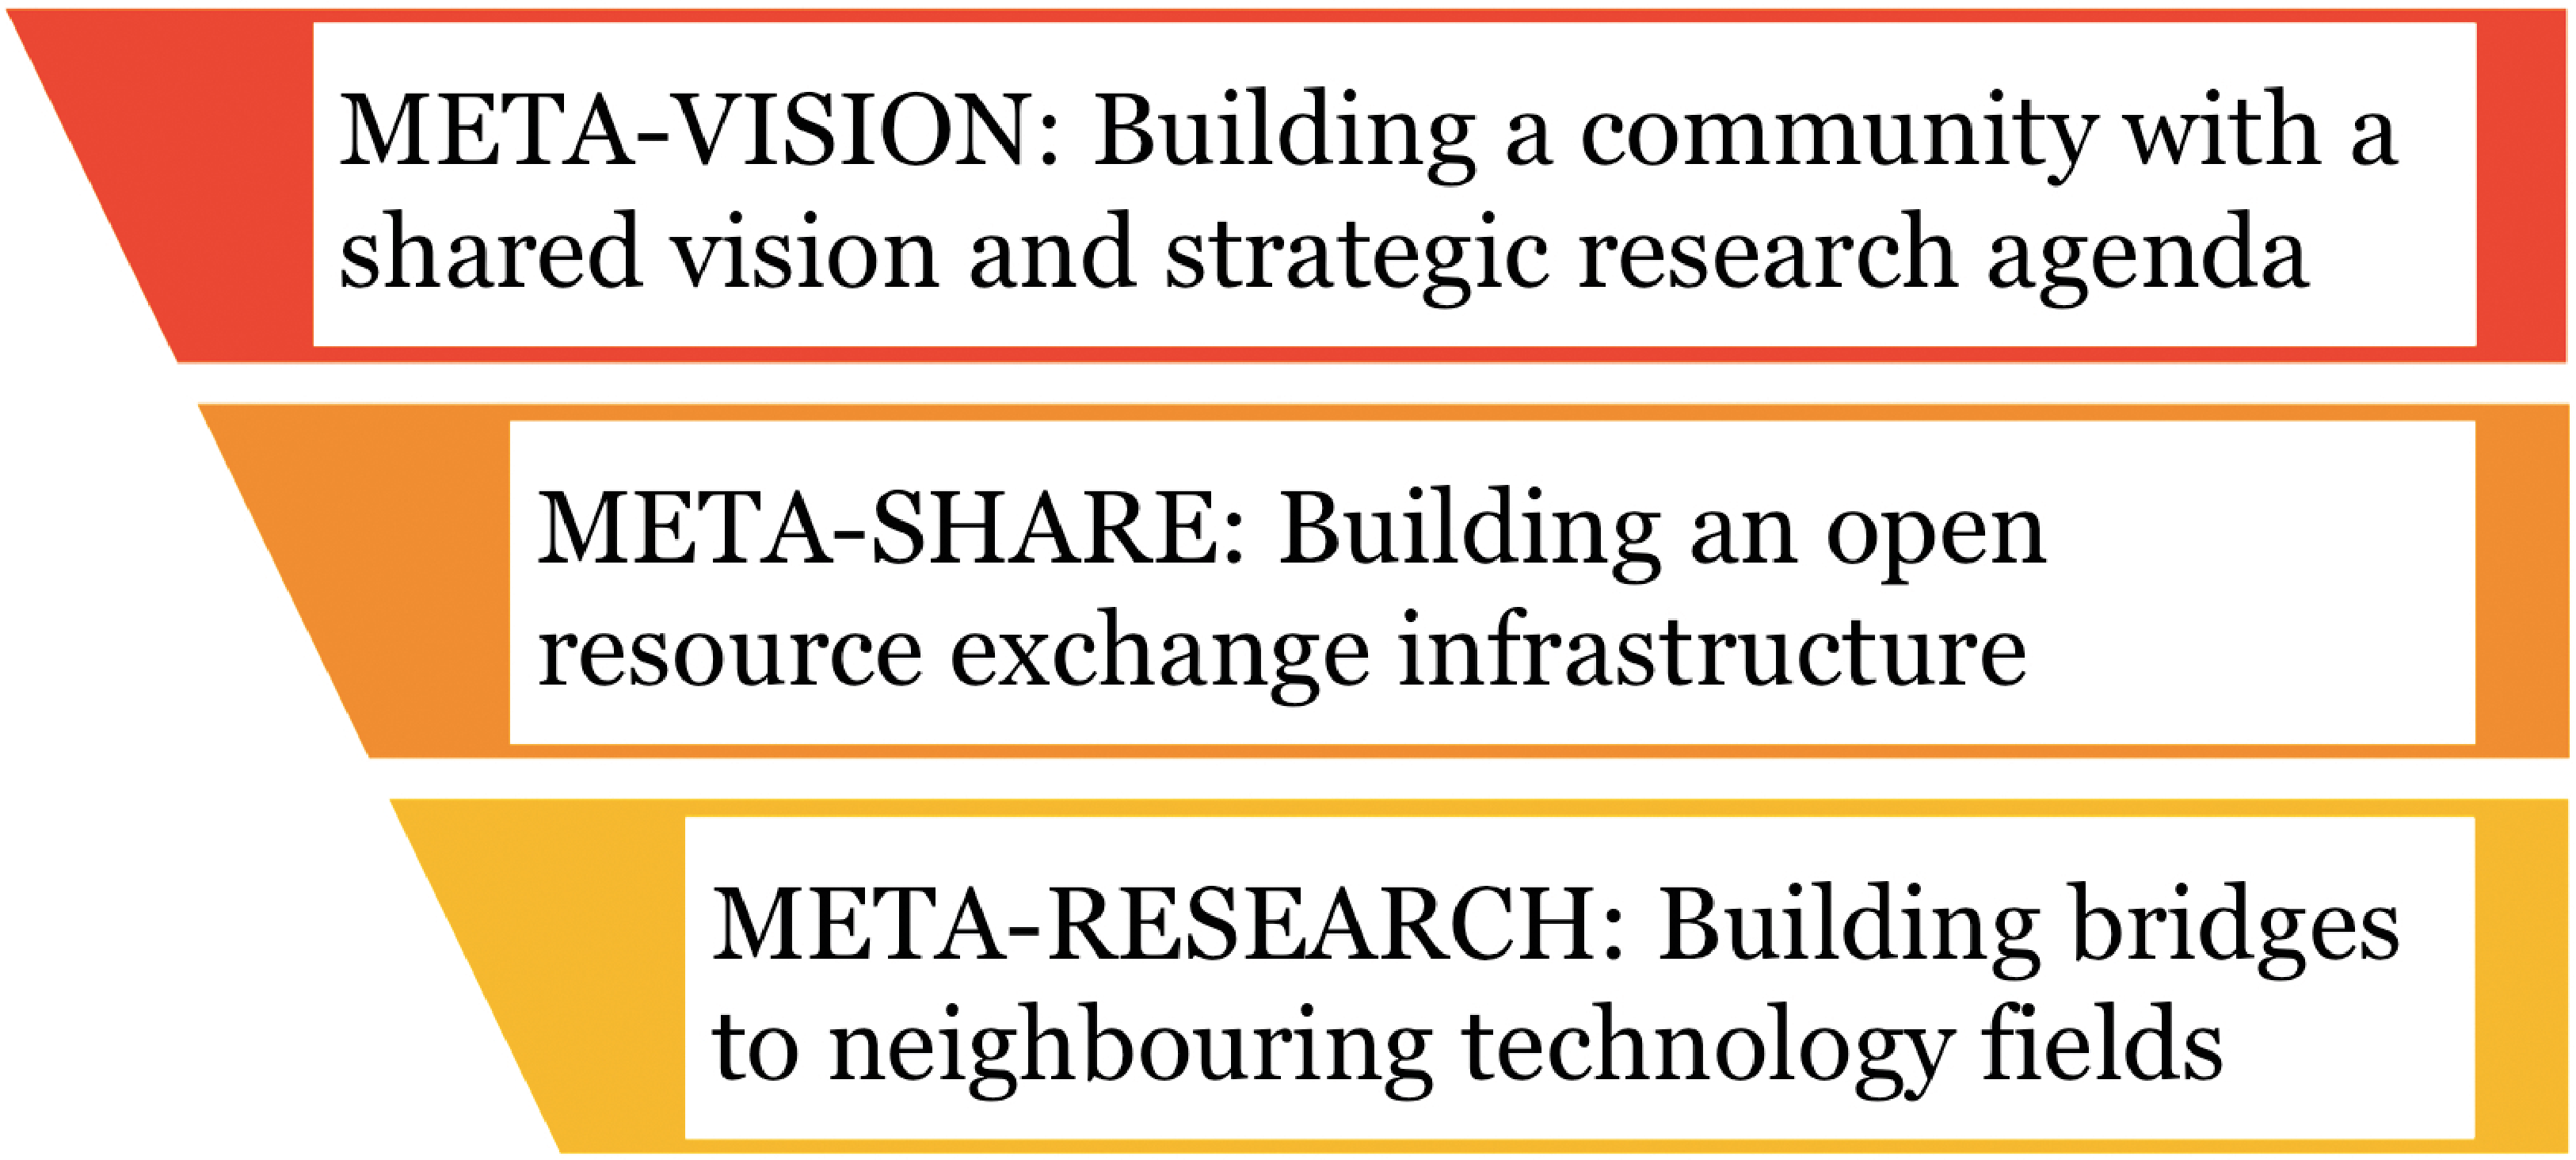
\includegraphics[width=0.42\textwidth]{../_media/action-lines}  
\end{center}

\vfill
%\centerline{office@meta-net.eu -- http://www.meta-net.eu}
\textbf{\centerline{office@meta-net.eu -- http://www.meta-net.eu}}
\end{multicols}

\clearpage

% ===========================================================================

\ssection[Members of META-NET]{Members of META-NET}
\label{metanetmembers}

\small

\begin{longtable}{@{}lp{137mm}@{}}
Austria & Zentrum für Translationswissenschaft, Universität Wien: Gerhard Budin\\ \addlinespace 
Belgium & Centre for Processing Speech and Images, University of Leuven: Dirk van Compernolle \\ \addlinespace
& Computational Linguistics and Psycholinguistics Research Centre, University of Antwerp: \newline Walter Daelemans\\ \addlinespace
Bulgaria & Institute for Bulgarian Language, Bulgarian Academy of Sciences: Svetla Koeva \\ \addlinespace
Croatia & Institute of Linguistics, Faculty of Humanities and Social Science, University of Zagreb: Marko Tadić \\ \addlinespace
Cyprus & Language Centre, School of Humanities: Jack Burston \\ \addlinespace
Czech Republic & Institute of Formal and Applied Linguistics, Charles University in Prague: Jan Hajič \\ \addlinespace
Denmark & Centre for Language Technology, University of Copenhagen: Bolette Sandford Pedersen, \newline Bente Maegaard\\ \addlinespace
Estonia & Institute of Computer Science, University of Tartu: Tiit Roosmaa, Kadri Vider\\ \addlinespace
Finland & Computational Cognitive Systems Research Group, Aalto University: Timo Honkela\\ \addlinespace
& Department of Modern Languages, University of Helsinki: Kimmo Koskenniemi, Krister Lindén \\ \addlinespace
France & Centre National de la Recherche Scientifique, Laboratoire d'Informatique pour la Mécanique et les Sciences de l'Ingénieur and Institute for Multilingual and Multimedia Information: Joseph Mariani \\ \addlinespace
& Evaluations and Language Resources Distribution Agency: Khalid Choukri\\ \addlinespace
& Laboratory of Computer Science, University of Le Mans: Holger Schwenk\\ \addlinespace
& Laboratoire Informatique d'Avignon, University of Avignon: Georges Linares\\ \addlinespace
Germany & Language Technology Lab, DFKI: Hans Uszkoreit, Georg Rehm\\ \addlinespace 
& Human Language Technology and Pattern Recognition, RWTH Aachen University: Hermann Ney \\ \addlinespace 
& Department of Computational Linguistics, Saarland University: Manfred Pinkal\\ \addlinespace
& Institute for Natural Language Processing, University of Stuttgart: Jonas Kuhn, Hinrich Schütze\\ \addlinespace
& Interactive Systems Lab, Karlsruhe Institute of Technology: Alex Waibel\\ \addlinespace 
Greece & R.C. “Athena”, Institute for Language and Speech Processing: Stelios Piperidis\\ \addlinespace
Hungary & Research Institute for Linguistics, Hungarian Academy of Sciences: Tamás Váradi\\  \addlinespace
& Department of Telecommunications and Media Informatics, Budapest University of Technology and Economics: Géza Németh, Gábor Olaszy\\ \addlinespace
Iceland & School of Humanities, University of Iceland: Eiríkur Rögnvaldsson\\ \addlinespace
Ireland & School of Computing, Dublin City University: Josef van Genabith\\ \addlinespace
Italy & Consiglio Nazionale delle Ricerche, Istituto di Linguistica Computazionale “Antonio Zampolli”: \newline Nicoletta Calzolari\\ \addlinespace
& Human Language Technology Research Unit, Fondazione Bruno Kessler:  Bernardo Magnini\\ \addlinespace 
Latvia & Tilde: Andrejs Vasiļjevs\\ \addlinespace  
& Institute of Mathematics and Computer Science, University of Latvia: Inguna Skadiņa\\ \addlinespace
Lithuania & Institute of the Lithuanian Language: Jolanta Zabarskaitė\\ \addlinespace
Luxembourg & Arax Ltd.: Vartkes Goetcherian\\ \addlinespace
Malta & Department Intelligent Computer Systems, University of Malta: Mike Rosner\\ \addlinespace
Netherlands & Utrecht Institute of Linguistics, Utrecht University: Jan Odijk\\ \addlinespace  
& Computational Linguistics, University of Groningen: Gertjan van Noord\\ \addlinespace
Norway & Department of Linguistic, Literary and Aesthetic Studies, University of Bergen: Koenraad De Smedt\\ \addlinespace  
& Department of Informatics, Language Technology Group, University of Oslo:  Stephan Oepen \\ \addlinespace
Poland & Institute of Computer Science, Polish Academy of Sciences: Adam Przepiórkowski, Maciej Ogrodniczuk \\ \addlinespace
& University of Łódź: Barbara Lewandowska-Tomaszczyk, Piotr Pęzik\\ \addlinespace
& Dept.~of Comp.~Linguistics and Artificial Intelligence, Adam Mickiewicz University: Zygmunt Vetulani \\ \addlinespace
Portugal & University of Lisbon: António Branco, Amália Mendes \\ \addlinespace 
& Spoken Language Systems Laboratory, Institute for Systems Engineering and Computers: Isabel Trancoso \\ \addlinespace
Romania & Faculty of Computer Science, University Alexandru Ioan Cuza of Iași: Dan Cristea \\ \addlinespace
& Research Institute for Artificial Intelligence, Romanian Academy of Sciences:  Dan Tufiș \\ \addlinespace
Serbia  & University of Belgrade, Faculty of Mathematics: Duško Vitas, Cvetana Krstev,  Ivan Obradović \\ \addlinespace
& Pupin Institute: Sanja Vranes \\ \addlinespace  
Slovakia & Ľudovít Štúr Institute of Linguistics, Slovak Academy of Sciences: Radovan Garabík \\ \addlinespace 
Slovenia & Jožef Stefan Institute: Marko Grobelnik \\ \addlinespace 
Spain & Barcelona Media: Toni Badia, Maite Melero \\ \addlinespace  
& Aholab Signal Processing Laboratory, University of the Basque Country:  Inma Hernaez Rioja \\ \addlinespace 
& Center for Language and Speech Technologies and Applications, Universitat Politècnica de Catalunya:  Asunción Moreno \\ \addlinespace 
& Department of Signal Processing and Communications, University of Vigo:  Carmen García Mateo \\ \addlinespace 
& Institut Universitari de Lingüística Aplicada, Universitat Pompeu Fabra: Núria Bel \\ \addlinespace 
Sweden & Department of Swedish, University of Gothenburg: Lars Borin \\ \addlinespace 
Switzerland & Idiap Research Institute: Hervé Bourlard \\ \addlinespace 
Turkey & Tübitek Bilgem: Mehmet Ugur Dogan \\ \addlinespace 
UK & School of Computer Science, University of Manchester: Sophia Ananiadou \\ \addlinespace  
& Institute for Language, Cognition and Computation, Center for Speech Technology Research, University of Edinburgh: Steve Renals \\ \addlinespace 
& Research Institute of Informatics and Language Processing, University of Wolverhampton:\newline Ruslan Mitkov \\ \addlinespace
& Department of Computer Science, University of Sheffield: Rob Gaizauskas\\ 
\end{longtable}
\normalsize

\renewcommand*{\figureformat}{}
\renewcommand*{\captionformat}{}

\begin{figure*}[h]
  \colorrule{grey3}{\textwidth}{1.5pt}
  \center
  %\fbox{-- META-NET group picture omitted to keep the size of the PDF file small. --}
  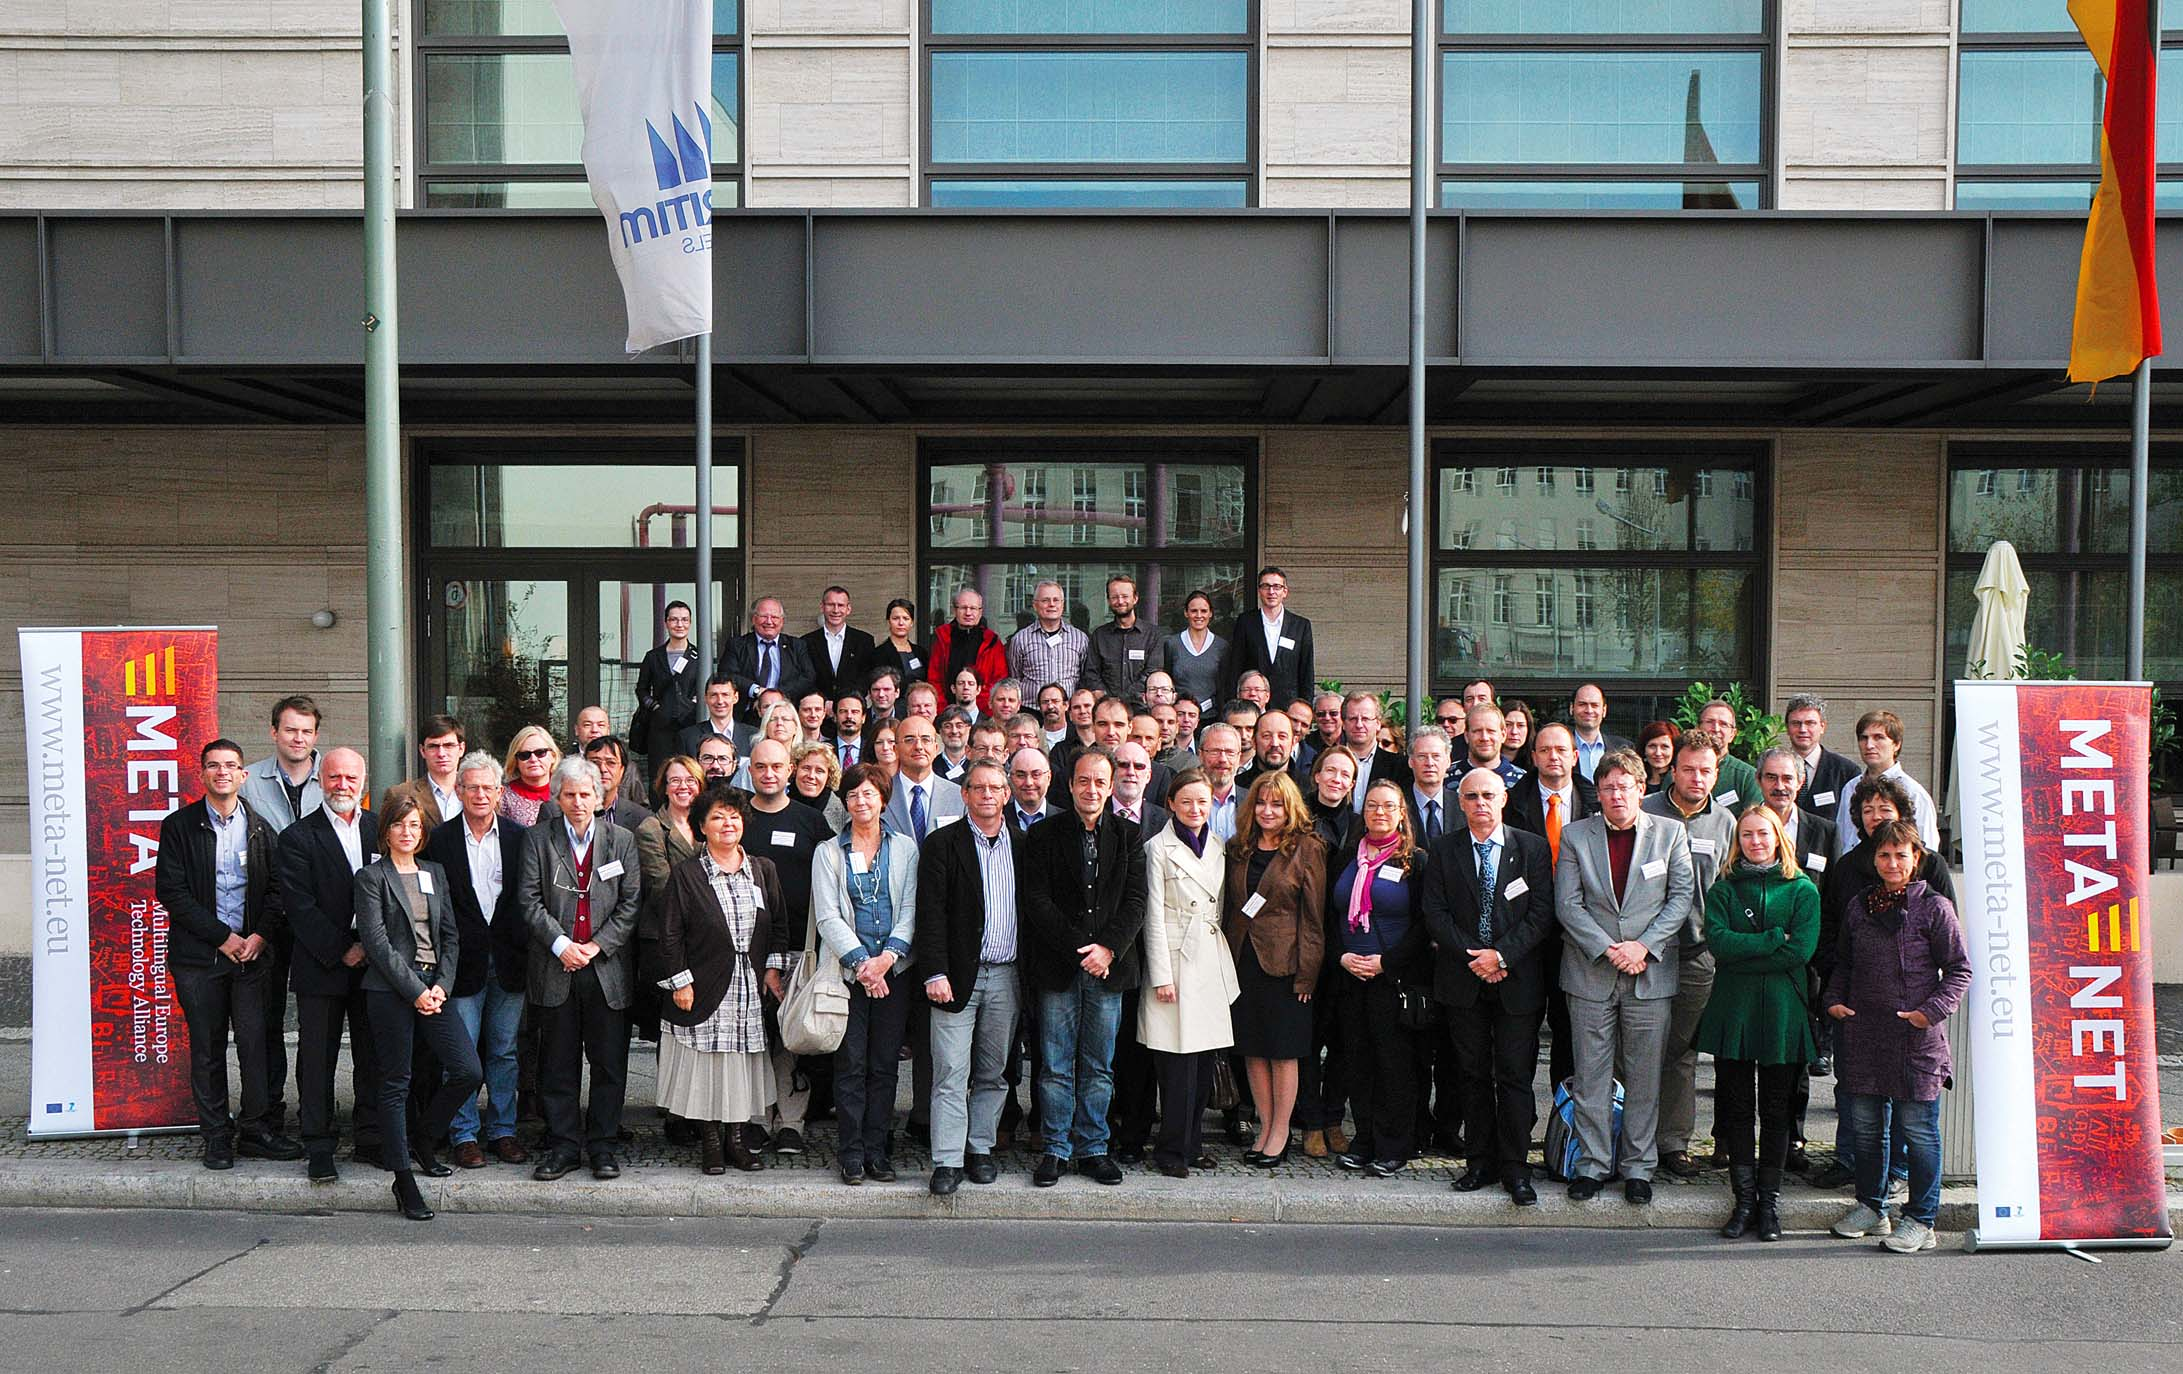
\includegraphics[width=\textwidth]{../_media/meta-net_team.jpg}
  \caption{About 100 language technology experts -- representatives of the countries and languages represented in META-NET -- discussed and finalised the key results and messages of the White Paper Series at a META-NET meeting in Berlin, Germany, on October 21/22, 2011.}
  \medskip
  \colorrule{grey3}{\textwidth}{1.5pt}
\end{figure*}

\clearpage

% ===========================================================================

%\ssection[Members of META]{Members of META}
%\label{metamembers}

% FIXME: Include a very tightly typeset list of the 630+ META members

%\clearpage

% ===========================================================================

\ssection[Milestones and History of the Strategic Research Agenda]{Milestones and History of the\newline Strategic Research Agenda}
\label{vision-evolution}

The META-VISION process within META-NET started in early 2010, its main aim was to produce this Strategic Research Agenda and the accompanying Roadmap document. Hundreds of representatives from academia, industry, official institutions, policy makers, politicians and journalists have contributed to this process. In this section we give an overview of the meetings at which the SRA or important components on the way towards the SRA have been presented and discussed (key meetings of the META-VISION process marked in bold typeface). 

Important milestones within the long and complex process towards this Strategic Research Agenda include five documents: the three Vision Reports prepared by the three domain-specific Vision Groups (see below), a general Vision Paper, ``The Future European Multilingual Information Society: Current State of the Discussion'' \cite{Meta1}, and the Priority Themes Paper in which the three technology visions are specified in a more concrete way, ``LT 2020 -- Vision and Priority Themes for Language Technology Research in Europe until the Year 2020. Towards the META-NET Strategic Research Agenda'' \cite{LT2020}. All reports, papers and discussions that took place in the process have been reflected in the Strategic Research Agenda. The documents are available online at \url{http://www.meta-net.eu/vision}.

% FIXME: Diese Liste evtl. ergänzen um die neuen Events, die bei allen Freunden und Partnern im Herbst 2012 durchgeführt worden sind?

\begin{small}
\begin{enumerate}
\item FLaReNet Forum, Barcelona, Spain, Feb.~11/12, 2010
\item Language Technology Days 2010, Luxembourg, March 22/23, 2010
\item EAMT 2010, Saint-Raphael, France, May 27/28, 2010
\item theMETAnk, Berlin, Germany, June 4/5, 2010
\item Translingual Europe 2010, Berlin, Germany, June 7, 2010
\item Localization World, Berlin, Germany, June 8/9, 2010
\item Multisaund Seminar, Istanbul, Turkey, June 16-18, 2010
\item \textbf{Vision Group ``Text Translation and Localisation''} (1st meeting), Berlin, Germany, July 23, 2010
\item \textbf{Vision Group ``Media and Information Services''} (1st meeting), Paris, France, Sep.~10, 2010
\item \textbf{Vision Group ``Interactive Systems''} (1st meeting), Paris, France, Sep.~10, 2010
\item ICT 2010, Brussels, Belgium, September 27-29, 2010
\item \textbf{Vision Group ``Text Translation and Localisation''} (2nd meeting), Brussels, Belgium, Sep.~29, 2010
\item \textbf{Vision Group ``Interactive Systems''} (2nd meeting), Prague, Czech Republic, Oct.~5, 2010
\item Languages and the Media 2010, Berlin, Germany, October 7, 2010
\item HLT: The Baltic Perspective, Riga, Latvia, October 7/8, 2010
\item LISA Forum Europe, Budapest, Hungary, October 13, 2010
\item \textbf{Vision Group ``Media and Information Services''} (2nd meeting), Barcelona, Spain, Oct.~15, 2010
\item EFNIL 2010, Thessaloniki, Greece, Nov.~3, 2010
\item Interact Presidential Summit, Moffett Field, USA, Nov.~8-9, 2010
\item \textbf{META Technology Council} (1st meeting), Brussels, Belgium, Nov.~16, 2010
\item Language question in research: English vs.~national languages?, Finnish Parliament, Helsinki, Nov.~17, 2010
\item \textbf{META-FORUM 2010: ``Challenges for Multilingual Europe''}, Brussels, Belgium, Nov.~17/18, 2010
\item Oriental-Cocosda 2010, Kathmandu, Nepal, Nov.~24-25, 2010
\item The International Workshop on Spoken Language Translation (IWSLT), Paris, France, Dec.~2/3, 2010
\item Meeting of the LT Berlin working group, Berlin, Germany, Dec.~9, 2010
\item Language Technology for Multilingual Applications, European Parliament, Luxembourg, Jan.~27, 2011
\item Opening of German/Austrian W3C Office at DFKI Berlin, Berlin, Germany, Feb.~10, 2011
\item Japanese Workshop for Machine Translation, Tokyo, Japan, Feb.~23, 2011
\item Meeting of Representatives of European Language Councils, Copenhagen, Denmark, March 08, 2011
\item TRALOGY, Paris, France, March 3/4, 2011
\item \textbf{Vision Group ``Interactive Systems''} (3rd meeting), Rotterdam, The Netherlands, March 28, 2011
\item \textbf{Vision Group ``Media and Information Services''} (3rd meeting), Vienna, Austria, April 1, 2011
\item Meeting of the LT Berlin working group, Berlin, Germany, April 4, 2011
\item W3C Workshop ``Content on the multilingual web'', Pisa, Italy, April 5, 2011
\item \textbf{Vision Group ``Translation and Localisation''} (3rd meeting), Prague, Czech Republic, April 7/8, 2011
\item Attensity Forum 2011, Berlin, Germany, May 6, 2011
\item \textbf{META Technology Council} (2nd meeting), Venice, Italy, May 25, 2011
\item FLaReNet Forum, Venice, May 26-27, 2011
\item Multisaund Seminar, Bursa, Turkey, June 13-14, 2011
\item META-NET Workshop at ICANN 2011: Context in Machine Translation,
Espoo, Finland, June 14, 2011
\item Speech Processing Conference, Tel Aviv, Israel, June 21-22, 2011
\item \textbf{META-FORUM 2011: ``Solutions for Multilingual Europe''}, Budapest, Hungary, June 27/28, 2011
\item Media for All, London, June 29-July 1, 2011
\item EUROLAN 2011 Summer School, Cluj-Napoca, Romania, Aug.~28-Sep.~4, 2011
\item Interspeech 2011, Firenze, Italy, Aug.~28-31, 2011
\item RANLP 2011, Hissar, Bulgaria, Sep.~12-14, 2011
\item Multilingual Web Workshop, Limerick, Ireland, Sep.~21/22, 2011
\item ML4HMT Workshop at MT Summit, Xiamen, China, Sep.~19-23, 2011
\item Workshop Language Technology for a Multilingual Europe at GSCL 2011, Hamburg, Germany, Sep.~27, 2011
\item GSCL 2011: ``Multilingual Resources and Multilingual Applications'', Hamburg, Germany, Sep.~28-30, 2011
\item \textbf{META Technology Council} (3rd meeting), Berlin, Germany, Sep.~30, 2011
\item Workshop on IPR and Metadata by META-NORD, Helsinki, Finland, Sep.~30, 2011
\item META-NET Network Meeting and General Assembly, Berlin, Germany, Oct.~21/22, 2011
\item NPLD Assembly, Eskilstuna, Sweden, Oct.~25/26, 2011
\item EFNIL 2011, London, UK, Oct.~26, 2011
\item Oriental-Cocosda 2011, Hsinchu, Taiwan, Oct.~26-28, 2011
\item SIMC 2011 International Symposium on Multilingualism in the Cyberspace, Brasilia, Brasil, Nov.~7-9, 2011
\item IJCNLP 2011, Chiang Mai, Thailand, Nov.~9-13, 2011
\item ML4HMT-11 Workshop, Barcelona, Spain, Nov.~19, 2011
\item LTC 2011, Poznan, Poland, Nov.~25-27, 2011
\item GALA Conference, Monaco, March 26-29, 2012
\item EACL 2012, Avignon, France, April 23-27, 2012
\item CESAR Roadshow Event, Sofia, Bulgaria, May 2, 2012
\item LREC 2012, Istanbul, Turkey, May 21-27, 2012
\item CESAR Roadshow Event, Bratislava, Slovakia, June 7/8, 2012
\item Multilingual Web Workshop, Dublin, Ireland, June 11, 2012
\item \textbf{META Technology Council} (4th meeting), Brussels, Belgium, June 19, 2012
\item \textbf{META-FORUM 2012: ``A Strategy for Multilingual Europe''}, Brussels, Belgium, June 20/21, 2012
\item CHAT 2012 Workshop, Madrid, Spain, June 22, 2012
\end{enumerate}
\end{small}

\begin{figure*}[htb]
  \colorrule{grey3}{\textwidth}{1.5pt}
  \center
  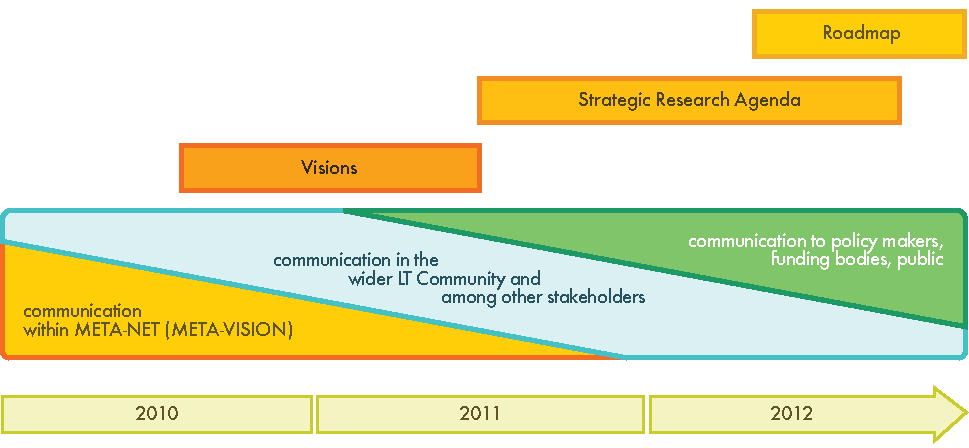
\includegraphics[width=0.65\textwidth]{../_media/Timeline}
  \caption{The three phases of the META-VISION process}
  \label{fig:sra-timeline}
  \colorrule{grey3}{\textwidth}{1.5pt}
\end{figure*}
 
\begin{figure*}[htb]
  \colorrule{grey3}{\textwidth}{1.5pt}
  \center
  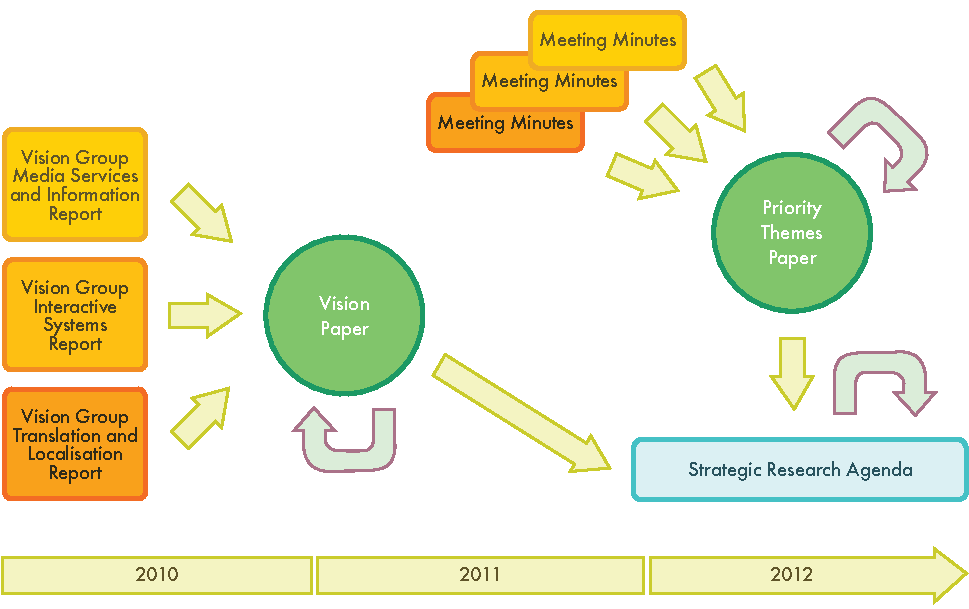
\includegraphics[width=0.65\textwidth]{../_media/Towards-SRA}
  \caption{Steps towards the Strategic Research Agenda for Multilingual Europe 2020}
  \label{fig:towards-sra}
  \colorrule{grey3}{\textwidth}{1.5pt}
\end{figure*}

\clearpage

% ===========================================================================

\ssection[Language White Paper Press Campaign: Overview and Impact]{Language White Paper Press Campaign: Overview and Impact}
\label{lwp-campaign}

% FIXME: Here, we could include graphics, Google Analytics data, more figures, examples, newspaper scans etc.

\textbf{Background:} META-NET prepared a study on the level of support that language technology provides for 30 European languages. The process took more than two years and resulted in 30 volumes of the META-NET White Paper Series “Europe’s Languages in the Digital Age”. More than 200 experts from academia and industry contributed as authors to this immense undertaking. Printed versions of the White Papers are published at Springer. PDF versions are available free of charge on \url{http://www.meta-net.eu/whitepapers}.

\smallskip
\textbf{Timeline:} At the beginning of September 2012, a press release was drafted at the META-NET Coordinator site, DFKI Berlin. This press release was translated and localised into 30 languages and, on September 20, sent out to national and international journalists, politicians and other stakeholder groups. Our goal was to gain traction in the online and traditional press on the occasion of the European Day of Languages which is traditionally held at September 26. The headline of our press release was:

\begin{center}
At Least 21 European Languages in Danger of Digital Extinction\\
Good News and Bad News on the European Day of Languages
\end{center}

\textbf{Response:} We were overwhelmed by the immediate, very big interest in the topic and our key findings. The first articles appeared online only hours after we sent out the first press releases. We also received multiple requests for radio and television interviews. Journalists called to collect additional statements and to enquire about specific details of our study. 

\smallskip
\textbf{Impact and Coverage:} We’re collecting and documenting all mentions in the traditional and online press and also radio and television reports on \url{http://www.meta-net.eu/whitepapers/press-coverage}. This collection process is ongoing. By now we estimate \textbf{ca.~300-350 mentions in the online press} in Europe and also multiple mentions in the international press (from Mexico to New Zealand). We also estimate that our press release generated more than 50 mentions in traditional newspapers. Representatives of META-NET took part in \textbf{about 25 radio interviews} (for example, in Germany, Greece, Iceland, Ireland, Latvia, Norway). We estimate that an \textbf{additional 25 radio and more than 15 television programmes} (including coverage in, for example, Iceland and Latvia) reported on our findings. 

\smallskip
\textbf{Examples:} A few significant newspapers and blogs that reported on us: Der Standard (Austria); Politiken, Berlingske Tidende (Denmark); Tiede (Finland); Heise Newsticker, Süddeutsche Zeitung (Germany); in.gr, Πρώτο Θέμα, Pro\-silip\-sis (Greece); Fréttablaðið, Morgunblaðið (Iceland); Wired (Italy); Computerworld (Norway); Delo, Dnevnik, De\-mo\-kra\-cija (Slovenia); El Mundo (Spain); Huffington Post (UK); Mashable, NBC News, Reddit (USA).

\clearpage

% ===========================================================================

% \ssection[Technologies for Europe's Languages: The Funding Situation]{Technologies for Europe's Languages:\newline The Funding Situation}
\label{european-funding-situation}

% FIXME: The following contains a collection of raw findings per language from the Language White Papers. The collection needs to be completed and the content still needs to be aggregated and integrated into the main text.

% FIXME: If we decide to keep this appendix we should write a short introduction to explain where this info is coming from.

\begin{multicols}{2}

\begin{small}
\subsection*{Basque}
\label{sec:basque}

Since 2000 up till today, the Spanish Government supported within the National Plan of Research and Technology several projects in the area of Multilingual Speech Technologies: TEHAM, AVIVAVOZ, and BUCEADOR. Their main purpose was to improve the quality of Speech Recognition, Speech Translation and Text to Speech Synthesis in all the official languages spoken in Spain: Basque, Galician, Catalan and Spanish.

\subsection*{Bulgarian}
\label{sec:bulgarian}

The first international and national funding supporting language technologies for Bulgarian began at the very beginning of 1990s. Over a short period of time financing for a number of research projects from European institutions was got: LaTeSLav (Language Processing Technologies for Slavic Languages, 1991-1994) aimed at developing a prototype of a grammar checker, BILEDITA (Bilingual Electronic Dictionaries and Intelligent Text Alignment, 1996-1998) for the development of bilingual electronic dictionaries, GLOSSER (Support of Second Language Acquisition and Learning from Aligned Corpora, 1996-1998) aimed at supporting foreign language training and others. The Multext-East (Multilingual Text Tools and Corpora for Central and Eastern European Languages, 1995-1997) extension of the previous Multext and EAGLES (European Commission’s Expert Advisory Group on Language Engineering Standards) EU projects provided the Bulgarian language resources in a standardised format with standard mark-up and annotation, and these resources were later expanded and upgraded in the ELAN (European Language Activity Network, 1998-1999), TELRI I in II (Trans European Language Resources Infrastructure, 1995-1998 / 1999-2001) and Concede (Consortium for Central European Dictionary Encoding, 1998-2000) projects. Bulgarian institutions are also involved in the CLARIN project (Common Language Resources and Technology Infrastructure). Other ongoing projects include those comprised by EUROPEANA aimed at developing the basic technologies and standards necessary to make knowledge on the Internet more widely available in the future.

\subsection*{Catalan}
\label{sec:catalan}

Machine translation, speech recognition, spelling and grammar checking research and industrial developments have been supported by different departments of the Generalitat de Catalunya for more than 20 years. The CREL – Centre de Referència en Enginyeria Lingüística, 1996-2000, managed by the Institut d’Estudis Catalans and with participants from the major Catalan Universities, was created with the specific aim of promoting the creation of resources and tools for the automatic processing of Catalan texts in a variety of applications. As regards the presence of the Catalan language in European infrastructures, in 2008 the Catalan Government signed an agreement with Universitat Pompeu Fabra, the national representative of the European project CLARIN in Spain, with the aim of building a Catalan demonstrator. In addition, the Biblioteca de Catalunya, Catalonia’s national library, is one of the partners in the EUROPEANA project. From 2000 up until the present day, the Spanish Government supported several projects in the area of multilingual speech technologies within the National Plan of Research and Technology, i.e., TEHAM, AVIVAVOZ, and BUCEADOR. The main purpose of these projects was to improve the quality of speech recognition, speech translation and text to speech synthesis in all the official languages spoken in Spain, i.e., Basque, Galician, Catalan and Spanish. In 2005, the Catalan Government launched a project to produce Language Resources for Speech Recognition and Speech Synthesis. As a result, Language Resources for telephone applications, in-car applications and microphone applications were produced. Later, the project TECNOPARLA (2007-2010) had as its objective the translation of speech between Spanish and Catalan. The project resulted on advances in all the component speech technologies, i.e. diarization, speech recognition, speech translation and text to speech synthesis.

%\subsection*{Croatian}
%\label{sec:croatian}
%
%n.\,a.

\subsection*{Czech}
\label{sec:czech}

Most of the government-originating funding programs are maintained by the Czech Science Foundation (GAÈR) and focused on basic research. Recently (2009), a new Technological Agency of the Czech Republic (Technologická agentura Èeské republiky, TAÈR) has been established, which shall focus on applied research. However, there are probably no LT-related projects funded by TAÈR yet. 

\subsection*{Danish}
\label{sec:danish}

The Research Council for the Technical Sciences had speech technology as one of the main themes in their strategy plan for 1998-2002, and they did support several language technology projects. The inter-disciplinary IT research programmes running from mid 1990s to 2003 have been able to support a few language technology related projects (as was the case for OntoQuery and SIABO), but have not had a specific aim to do so.
The Research Agency of the Danish Ministry for Science, Technology and Development decided in 2001 to promote language technology by funding a collaborative effort to enlarge the Danish language technology lexicon developed in the European PAROLE project. The resulting dictionary (STO) is now available through ELRA, and is being used for research and commercial purposes. It was the specific aim of the Research Agency to support the Danish language in the digital age, by granting funds for the development of basic language technology building blocks.
In parallel with the ESFRI initiative for research infrastructure, Denmark has started a roadmap process for research infrastructures. One of the research infrastructures to be supported will be a “Digital Humanities Laboratory” for the support of humanities research through the use of language technology.

\subsection*{Dutch (Netherlands, Flanders)}
\label{sec:dutch-neth-fland}

Activities for the Dutch language have been promoted and supported in several programmes and projects over the last one and a half decade. Thus a Dutch language spoken train information system was developed as a carrier for research in speech analysis and generation, in language analysis and generation, and in dialogue management in the OVIS programme in the late nineties. 

METAL produced a Dutch-French MT system for the ministries of Agriculture and Internal Affairs, and after the Dutch Language Union issued a call for the development of MT systems translating between Dutch on the one hand and English and French on the other in 1999, funded by public money, Systran developed such systems in the context of the NL-Translex project. In the IOP MMI (Innovation Research Programme on Man Machine Interaction) and CATCH programs language and speech technology have been used as tools for man machine interfaces and disclosing cultural heritage.

Most prominent in their focus on the Dutch language are the joint Netherlands-Flanders CGN and STEVIN programmes. These have yielded significant progress in the availability of basic resources (data and tools) for the Dutch language, some initial research and several end user applications. Though some of the results achieved in these projects can be exploited in industry and in academia (e.g. in the CLARIN-NL research infrastructure) the prospects for optimally exploiting these results in actual research and in industry further are grim. 

\subsection*{English}
\label{sec:english}

AKT (2000-2007), was a multi-million pound collaboration between five UK universities, with the aim of enhancing information and knowledge management in the age of the World Wide Web. The research conducted on the project formed an important contribution to the semantic web, in which the use of LT technologies played a central role. A follow-up project, ”EnAKTing the Unbounded Data Web: Challenges in Web Science”, is currently ongoing.
Two systems which support the user in creating new applications from existing libraries of processing components are the University of Sheffield’s GATE system, which has been under development for over 15 years, and the more recent UCompare system, which was developed as part of a collaboration between the Universities of Tokyo, Manchester and Colorado. Whilst current components in UCompare mainly deal with English, the library will be extended as part of META-NET to cover a number of different European languages.

%\subsection*{Estonian}
%\label{sec:estonian}
%
%n.\,a.

\subsection*{Finnish}
\label{sec:finnish}

Public support from TEKES has been an important source of funding for basic research especially through two large technology programs, USIX (User-Oriented Information Technology) 1999--2002 and FENIX (Interactive Computing) 2003--2007. Some of the core technologies identified in the program in UNIX were Finnish speech recognition, large data management and search interfaces.

NLP projects carried out within the FENIX technology program include FENIX 4M (Mobile and Multilingual Maintenance Man) and FinnONTO (Semantic Web Ontologies) at the University of Helsinki, New methods and applications in speech processing and Search-in-a-Box (University of Turku), Rich semantic media for personal and professional users (VTT Technical Research Centre of Finland) and Intelligent Web Services (Helsinki School of Science and Technology), StatHouse Semantics and Automatic content classification and ontologies (Seerco Ltd).  Recently, A joint project on speech synthesis between the University of Helsinki and Aalto University has been very successful in the new field of statistical parametric synthesis based on Hidden Markov Models and a new, physiologically grounded vocoding technology.

EU funded projects in Finland since the 1980’s include LR SIMPLE, LR PAROLE and EU MLIS 5008 LINGMACHINE. The Common Language Resources and Technologies Infrastructure (CLARIN) was funded by the Commission during 2008 - 2010, and the work within the initiative continues. The national part FINCLARIN is funded by the Ministry of Education and Culture.  HFST (Helsinki Finite State Transducer Technology), OMor (Open Source Morphologies), FinnWordNet, and FinnTreeBank are examples of currently ongoing projects.

\subsection*{French (France, Belgium, Switzerland, Canada)}
\label{sec:french-france-belg}

As a follow-up of the FRANCIL program of the AUPELF-UREF (Francophone Universities Association) from 1994 to 2000, the Techno-Langue program (2003-2005), supported by the Ministries of Research, Industry and Culture, included the development of Language Resources (corpus, lexica, dictionaries, etc.) for French and the organization of 8 evaluation campaigns, on topics such as Syntactic Parsing, Text Alignment, Machine Translation, Terminology Extraction, Information Retrieval (Question \& Answer), Broadcast News speech transcription (ESTER campaign), Text-to-Speech Synthesis and Spoken dialog. The ESTER campaign allowed producing, in 2004, 1,700 hours of Broadcast News speech in French, 100 hours of which have been transcribed, making it possible to develop Broadcast News transcription systems of sufficient quality and opening the feasibility of automatic video transcription and indexing for French.  Some of those activities are now continuing as individual projects supported by the ANR (ETAPE, PASSAGE, PORT MEDIA), which also organized the REPERE challenge on multimodal (text, speech and vision) person identification (2010-2013).

CNRS (the National Centre for Scientific Research) had several programs in that field along the years, and the French Ministry for Research settled in 2011 a Corpus Infrastructure in the Human and Social Sciences area, in connection with the EC CLARIN project.

Nowadays, OSEO supports the very large Quaero program gathering 31 industrial and academic partners (French and German) with a total budget of 200 M. and an amount of public funding of 99 M. over 5 years (2008-2013). Quaero addresses the development of around 30 technologies for various medias (speech, text, music, image, video) for the needs of 8 applications related to Multimedia and Multilingual Document processing (Digitization platform, Multimedia Entreprise Capture, Social impact media monitoring, Personalized video, Communication portals \& Digital Heritage, Online Translation Platform, Real Life Mobile Search and Multimedia search engines). All technologies are developed under a strict, regular quantitative evaluation scheme, while a special project produces the data that is necessary for developing and testing the technologies. Although the program mostly addresses the French language, some technologies will be developed for most of the 23 EU official languages. The Voxalead News online application developed by Dassault/Exalead in cooperation with LIMSI-CNRS, Vocapia Research and INRIA is a good example of a major technological achievement made possible within Quaero by gathering know-how in three different areas (search engines, speech processing and image processing). 

In Belgium, the Service de la langue de la Communaute francaise de Belgique has funded the development of terminological researches in the past and is officially in charge of coordinating the terminological activities (at the government level) in the Francophone part of Belgium. The OWIL (Observatoire du Traitement Informatique des Langues et de l’Inforoute) has centralized information on NLP research and activities for several years, but has stopped its activities in 2008.

There is currently no major LTR program in Switzerland.  The most relevant project may be the National Centre of Competence in Research on Interactive Multimodal Information Management (IM2), lead by IDIAP, where speech corpora have been collected, mainly in collaboration with the EC AMI and AMIDA projects. There used to be an “observatoire” for research, but the site is now inactive. 

Canada has a special agency for HLT: the LTRC (Language Technology Research Center) / CRTL (Centre de Recherche en Technologies Langagières). There are in Canada several academic teams working on HLT, but without any specific national program, apart from generic national research programs.

\subsection*{Galician}
\label{sec:galician}

The Centre for the Development of Industrial Technology (CDTI) is a Spanish public organisation, under the Ministry of Science and Innovation, whose objective is to help Spanish companies increase their technological profile. CDTI evaluates and finances R\&D projects through programmes such as CENIT and AVANZA.

The CENIT (National Strategic Consortiums for Technological Research) programme seeks to stimulate public and private-sector cooperation in R\&D. Information Technology and Communication is one of the programme’s priority areas. Projects in this area sometimes include research in Language Technologies.

The aim of the AVANZA Plan is to bring the Information Society to ordinary citizens, and to private and public sectors. Among their priorities is to facilitate the use of new technologies to elderly people and people with disabilities. User-friendly language technology tools offer the principal solution to satisfy this goal, for example by offering speech synthesis for the blind.

The Galician Regional Government supports research through the “Plan Galego de Investigación, Desenvolvemento e Innovación Tecnolóxica (PGIDIT)”. Language Technology is not a priority line, but along the years research groups from the universities and some companies have gotten grants for doing research and developments in LT.

\subsection*{German (Germany, Austria, Switzerland)}
\label{sec:germ-germ-austr}

COLLATE, funded by the BMBF from 2000 to 2006, was one of the first projects to address the issues of a language infrastructure and led to the creation of an information portal for the field (LT World). German and Austrian institutions are involved in the on-going European CLARIN project. Other on-going projects include EUROPEANA and THESEUS, a project co-funded by the Federal Ministry of Economics and Technology (BMWI) that aims to develop the basic technologies and standards needed to make knowledge on the Internet more widely available in the future.

In Austria, the Faculty of Computer Sciences at the University of Vienna is carrying out the JETCAT project on translation between Japanese and English, and an on-going project has been compiling the Austrian Academy Corpus since 2001. There are no dedicated LT programmes in Austria. Funding for LT-related topics typically comes from research programmes that have open topics, especially those that focus on the transfer of knowledge from academic research to industry (particularly via SMEs). Several of these programmes are administered by the Austrian Research Promotion Agency (FFG). The Vienna Science and Technology Fund (WWTF) is a fairly strong supporter of localised LT, especially for topics related to Vienna, such as synthesizing the speech of the Viennese dialect (or sociolect) and building MT systems to translate from Austrian German to Viennese and other dialects.

In Switzerland, interest in language technology began in the 1980s with strong involvement in the EUROTRA project. The Universities of Zurich and Geneva are currently working on several projects in the field of MT including MT between Standard German and Swiss German. Corpus-building projects include the collection of speech corpora by the National Centre of Competence in Research on Interactive Multi- modal Information Management and a project that collects SMS text messages in Swiss German. Generally speaking, Switzerland has a small LT sector, mainly because of limited funding opportunities. 

\subsection*{Greek}
\label{sec:greek}

A significant asset gained by previous funding initiatives is the establishment of a group of LT teams in major Research Centers and University labs as well as of LT aware teams in companies. Most of these teams are continuously active in the area through EU research activities and have acted positively in producing most of the LT resources and tools that are now available for Greek, covering the axes of text, speech and multimedia data processing. A new national all-areas R\&D funding initiative (SYNERGASIA) is currently unfolding, including some promising LT projects. Since this programme is built to foster academia-industry collaborations, it is foreseen that a good set of Greek language tools and LT enhanced systems and services will be available in the coming years.

\subsection*{Hungarian}
\label{sec:hungarian}

In recent years, the international trends of standardisation and uniformisation of existing resources have reached Hungary as well. Several projects started off with the objective of integration and interoperability, e. g. creating a unified Hungarian ontology, or harmonising the different coding systems of separately developed morphological analysers. In 2008, prominent Hungarian academic institutions and R\&D companies formed the Hungarian Platform for Speech and Language Technology, which aims to help sharing and integration of high quality knowledge accumulated in centres that worked in isolation beforehand; to work out detailed strategic and implementation plans and to help their subsequent implementation; to disseminate its analyses and proposals among the members of the IT sector; to represent the Hungarian interests at the international level; and to disseminate the achievements of the Platform among the potential users of the technology. Hungarian institutions have also been involved in the CLARIN project.

\subsection*{Icelandic}
\label{sec:icelandic}

In 2000, the Icelandic Government launched a special Language Technology Programme with the aim of supporting institutions and companies in creating basic resources for Icelandic language technology. This initiative resulted in several projects which have had profound influence on the field in Iceland. After the Language Technology Programme ended in 2004, researchers from three institutes (University of Iceland, Reykjavik University, and the Arni Magnusson Institute for Icelandic Studies), who had been involved in most of the projects funded by the programme, decided to join forces in a consortium called the Icelandic Centre for Language Technology (ICLT), in order to follow up on the tasks of the programme. Since 2005, the ICLT researchers have initiated several new projects which have been partly supported by the Icelandic Research Fund and the Icelandic Technical Development Fund. The most important product of these projects is the open source IceNLP package (IceTagger, IceParser and Lemmald) which is also available as an online service (http://nlp.cs.ru.is). In 2009, the ICLT received a relatively large three year Grant of Excellence from the Icelandic Research Fund to the project ‘Viable Language Technology beyond English – Icelandic as a test case’. Within that project, further basic LT resources for Icelandic are being developed.

\subsection*{Irish}
\label{sec:irish}

Ireland is home to a number of leading research institutions in the field of computational linguistics, and has a National Centre for Language Technology located at Dublin City University alongside the Centre for Next Generation Localisation, which works on using computational linguistics to bring added value to globalisation, localisation and information access. Both of these centres are well established and have strong links with industrial R\&D both locally and abroad, as well as strong ties with other European centres of excellence in the field. The machine translation research team based at the CNGL is among the largest and most successful in the world. 

% No info about funding situation.

\subsection*{Italian}
\label{sec:italian}

As for Italian, a considerable effort has been invested in Language Technologies research in Italy since 1997, when Human Language Technology (hence forth HLT) was designated a National research policy, with the launch of two three-year projects: TAL (National Infrastructure for Linguistic resources in the field of Automatic Treatment of Spoken and Written Natural Language), funded by the Italian government for about 1.75M Euros and LRCMM, devoted to mono and multilingual research in computational linguistics, funded for about 3M Euros. Since the two projects above were launched, only two small-size projects have been recently funded, i.e. MIUR-PARLI, for the harmonization of existing computational resources for Italian, and MIUR-PAISA, for the realization of a platform for learning Italian from annotated corpora. The majority of the production of language resources and technologies for Italian is the result of various EU-funded research projects and other initiatives. Italian groups are involved, often with coordination roles, in international networking projects, particularly at the European Level (for example in CLEF, the Cross Language Evaluation Forum, and in FLaReNet, a project fostering an international network for language resources). According to a recent META-NET survey, there are currently seven national projects running and six European projects coordinated by Italian partners.

%\subsection*{Latvian}
%\label{sec:latvian}
%
%n.\,a.

\subsection*{Lithuanian}
\label{sec:lithuanian}

Most of the initiative and commitment with regard to the functioning of the Lithuanian language within the information society and LT development originates on the national level. The year 2000 saw the launch of the first national programme of the Lithuanian language in the information society for the period of 2000–2006, coordinated by the State Commission of the Lithuanian Language. The Information Society Development Committee under the Ministry of Transport and Communications is responsible for the second phase of the program of the Lithuanian Language in the Information Society 2009-2013. The programme provides for the creation of an Internet portal with free access to all the available language resources and technologies, augmentation of the existing and newly created linguistic resources, improvement of the ASR and TTS technologies, new MT tools, improvement and development of semantic and syntactic analysis and search tools.

The Lithuanian Research Council has launched the first national program ”State and Nation: Heritage and Identity” that encompasses digitalization of intangible heritage (this program saw the implementation of the project called ”Development of a Lituanistic Digital Resource Metadata System out its Compatibility with CLARIN”).  Recently, The Lithuanian Council of Sciences also finances the programme for the Development of National Lituanistics 2009–2015, aimed at developing and promoting lituanistic research, helping meet the priority of lituanistic research, strengthening the input of lituanistic research data into the overall expansion of nation-wide humanistic, providing a scientific base for nurturing national self-consciousness and protecting lituanistic heritage.

\subsection*{Maltese}
\label{sec:maltese}

The government’s National IT Strategy 2008-10 included a number of objectives related to Maltese Language including (i) the development of online government in Maltese, (ii) creation of Maltese language tools, in collaboration with the University, and (iii) support for Maltese online communities.  Currently the language technology scene in Malta is under the influence of four main initiatives: 1.~A government-supported project partly funded by EU regional development funds is under way to bring speech technology within the reach of disabled persons. The project is currently focused on Maltese speech synthesis.  2.~Malta participates in METANET4U and is thus in receipt of significant EU funding aimed at the enhancement and distribution of resources and tools that are specifically for Maltese.  3.~The Maltese Language Resource Server (MLRS) has come to fruition and significant efforts are under way at University, through the Institute of Linguistics and the Department of Intelligent Computer Systems, to maintain and develop it.  4.~Finally, a new undergraduate programme in Human Language Technology is destined to be launched by the Institute of Linguistics in October 2011.  Besides these, a project to develop an electronic version of the Aquilina dictionary is currently in preparation.

\subsection*{Norwegian}
\label{sec:norwegian}

The Research Council of Norway has supported one language technology research program, namely KUNSTI (Kunnskapsutvikling for norsk språkteknologi). It was in part inspired by larger projects in other countries (e.g. the German project Verbmobil) and aimed to increase competence in language technology through basic research. KUNSTI aimed for R\&D to make spoken and written Norwegian in various forms (and to some extent Saami) accessible for computer processing. Twenty research projects of varying sizes were completed under the program, the largest two being in MT and speech processing.

It was an important achievement to establish the Language Technology Resource Collection for Norwegian – Språkbanken in 2010, after two decades of joint efforts between the Norwegian Language Council, the Research Council, commercial companies and the Norwegian research institutions. Språkbanken at the National Library is to function as an infrastructure for making Norwegian LRT available for research and commercial use, thus hopefully reducing the threshold for developing Norwegian LRT products. Sizeable LRT building projects (e.g. the INESS, NoTa-Oslo (Norsk Talespråkskorpus, the Oslo part), Norsk aviskorpus, WeSearch—Language technology for the web and SIRKUS) after KUNSTI have been financed through infrastructure programs (AVIT) or general ICT programs from the Research Council such as VERDIKT. As a part of building basic Norwegian LRT, Språkbanken signed a contract with Kaldera språkteknologi AS in 2011 to create wordnets for Norwegian.

%\subsection*{Polish}
%\label{sec:polish}
%
%n.\,a.

\subsection*{Portuguese (Portugal, Brazil)}
\label{sec:port-port-braz}

In the field of speech processing, it is worth noting the TECNOVOZ project, which started in 2006. This project was directed by INESC-ID and one of its major goals was to foster technology transfer to the business sector, having as partners companies like the public television RTP.  Portuguese and Brazilian institutions have been participating in the ongoing CLARIN project, aiming at establishing an integrated and interoperable European research infrastructure of language resources and technology.  In Portugal, funding for language technology comes mainly from the Ministry of Science, Technology and Higher Education, through the Foundation for Science and Technology (FCT). However, obtaining support for language technology projects is particularly difficult, if not impossible, because project proposals in this area are accepted and evaluated under the Electrical Engineering track in calls for project proposals, where they have to compete with hundreds of proposals on totally unrelated issues and face evaluation committees disconnected from the area and its research topics. On a par with FCT, the Fundação Calouste Gulbenkian occasionally funds some language technology projects.

In Brazil, the FAROL Project (2006-2010), developed and conducted by the Pontifical Catholic University of Rio Grande do Sul, aimed at reinforcing the cooperation links among teams in Brazil, promoting students and researchers interchange and better research quality in natural language processing.  In Brazil, funding for research, in general, and for language technology activities, in particular, is still limited and comes mainly from government agencies. The National Council for Scientific and Technological Development (CNPq), the Sao Paulo Research Foundation (FAPESP), the Coordination for Advancement of High Education Personnel (CAPES), and the Funding Agency for Studies and Projects (FINEP) are the four institutions that significantly support research in this country. Some of these agencies have provided also special joint university-industry funding programs. For instance, FAPESP and Microsoft Research recently formed a partnership to fund socially relevant projects in the state of Sao Paulo, which included, for instance, the PorSimples text simplification project in the area of language technology.

\subsection*{Romanian}
\label{sec:romanian}

Previous national programs have led to an initial impulse, but subsequent financial aid missing or not attractive enough has lead to a loss of interest from major ICT players and young researchers, formed by universities and the Academy. One of the programs of collaboration between industry and education that has a good impact and results in Romania is the MSDN Academic Alliance, offering students free access to different Microsoft technologies.

As for research programs, UAIC and RACAI have been involved in several national or international research programs, intended to develop existing or new language technologies. Many of the conducted projects were European funded. Some nationally funded projects also existed, such as: STAR (A System for Machine Translation for Romanian), SIR-RESDEC (Open Domain Question Answering System for Romanian and English), ROTEL (intelligent systems for the Semantic Web, based on the logic of ontologies and NLP), eDTLR (The Romanian Thesaurus Dictionary in electronic form), among others.

\subsection*{Serbian}
\label{sec:serbian}

The first interdisciplinary project entitled “Interactions between text and dictionaries” was conceived in 2002 as a joint project of the Departments of Serbian at the Faculty of Philology in Belgrade and the Faculty of Philosophy in Novi Sad, as well as the Faculty of Mathematics in Belgrade. In the scope of this project the first corpus of contemporary Serbian was developed and the development of an electronic morphological dictionary of Serbian following the so-called LADL format was initiated.  The project was later continued as a joint project of the Department of Serbian at the Faculty of Philology and the Faculty of Mathematics in the period from 2006 to 2010 under the name “A theoretical and methodological framework for the modernization of Serbian” and from 2011 to 2014 under the name “Serbian and its resources: theory, description and applications”. Within the scope of these projects the development of the electronic dictionary of simple words was finalised, and the development of the dictionary of compounds initiated, aligned French-Serbian and English-Serbian corpora of literary texts were developed, as well as local grammars for certain segments of Serbian (especially for named entities). Different software tools were also developed, among which special attention should be given to LeXimir, a workstation which enables integration and transformation of heterogeneous lexical resources.

Parallel with this research in the field of language, a project was funded within the social sciences field under the name “Fundamental cognitive processes and functions”, realised by the Department of Psychology at the Faculty of Philosophy in Belgrade. The aim of this project, among other things, was to investigate the possibility of the automatic annotation of texts based on an annotated corpus.  Speech synthesis and recognition is being realised at the Faculty of Technical Sciences of the University of Novi Sad through projects of technological development from 2005, namely “Development of speech technologies in Serbian and their application in Telekom Serbia” (2005-2007), “Man-machine speech communication” (2008-2010), “Development of dialogue systems for Serbian and other South-Slavic languages” (2011–2014). They provide support for different TTS and ASR applications and services including IVR systems, private branch exchanges, call centres, audio logging, track commercials, word spotter, etc.  In addition to national projects, Serbian scientific institutions have also taken part in various international projects related to the HLT field.

%\subsection*{Slovak}
%\label{sec:slovak}
%
%n.\,a.

\subsection*{Slovene}
\label{sec:slovene}

In general, it can be stated that in the last two decades language technology for Slovene was never supported by a consistently devised national funding scheme. The process of the development of HLT applications, tools and resources for Slovene has been therefore a mixture of international projects extending their scope from Western European languages to Central and Eastern Europe with a view toward the EU enlargement process, national research funding where speech interaction was the dominant research area, and the enthusiasm of individuals involved in LT or of larger groups working on the localization of free software such as Linux, OpenOffice, etc., to Slovene.  In the 2000s, the Alpineon software company, a spin-off from the Faculty of Electrical Engineering (University of Ljubljana) led a large consortium in the Voicetran project (2004-2008), the biggest national speech interaction project to date.  A new standardization effort concerning a morpho-syntactic tagging system, with origins in the MULTEXT-East project and used in the annotation of the FIDA line of corpora, and a newly developed syntactic annotation system was funded in the JOS project (Linguistic annotation of Slovene 2007--2009). The results of the project are now used in a large European Social Fund project “Communication of Slovene” (2008--2013), led by the Amebis software company, where a new tagger and parser is being developed along with an upgrade of the FidaPLUS corpus to more than 1 billion word Gigafida corpus.  Statistical data on national research funding shows that 18 national research projects were funded in the field of speech interaction from 1995 to 2010, 9 in the field of written language technologies and 3 in the digitization of (historical) resources. However, language technology as a field has never seen a more consistent national effort in the sense of building a LT language infrastructure for Slovene, exemplified by the German COLLATE project or TST Centrale for Dutch.

%\subsection*{Spanish}
%\label{sec:spanish}
%
%n.\,a.

%\subsection*{Swedish}
%\label{sec:swedish}
%
%n.\,a.
\end{small}

\end{multicols}

\clearpage



% ===========================================================================

\ssection[Abbreviations and Acroynms]{Abbreviations and Acronyms}
\label{sec:acronyms}

% Reference acronyms with \acs{AI} or \acl{AI} (acs: short form; acl: long form)

\begin{multicols}{2}
  \begin{acronym}
    \acro{AI}{Artificial Intelligence}
    \acro{API}{Application Programming Interface}
    \acro{CALL}{Computer-Assisted Language Learning}
    \acro{CAT}{Computer-Aided Translation}
    \acro{CEF}{Connecting Europe Facility} 
    \acro{CMS}{Content Management System}
    \acro{EFNIL}{European Federation of National Institutions for Language}
    \acro{ETP}{European Technology Platform}
    \acro{GALA}{Globalization and Localization Association}
    \acro{GPS}{Global Positioning System}
    \acro{HQMT}{High-Quality Machine Translation}
    \acro{HLT}{Human Language Technology}
    \acro{HTML}{Hypertext Markup Language}
    \acro{IaaS}{Infrastructures as a Service}
    \acro{IR}{Information Retrieval}
    \acro{ISO}{International Organization for Standardization}
    \acro{ICT}{Information and Communication Technology}
    \acro{IT}{Information Technology}
    \acro{JTI}{Joint Technology Initiative}
    \acro{LR}{Language Resource}    
    \acro{LSP}{Language Service Provider}    
    \acro{LT}{Language Technology}
    \acro{META}{Multilingual Europe Technology Alliance}
    \acro{MT}{Machine Translation}
    \acro{NLP}{Natural Language Processing}
    \acro{NPLD}{Network to Promote Linguistic Diversity}
    \acro{PaaS}{Platforms as a Service}
    \acro{PHP}{PHP: Hypertext Preprocessor}
    \acro{PPP}{Public-Private Partnership}
    \acro{RSS}{RDF Site Summary; Really Simple Syndication}
    \acro{SME}{Small and Medium Enterprises}
    \acro{SaaS}{Software as a Service}
    \acro{SRA}{Strategic Research Agenda}
    \acro{TFEU}{Treaty of the Functioning of the European Union}
    \acro{TM}{Translation Memory}
    \acro{TMS}{Translation Management System}
    \acro{WWW}{World Wide Web}
    \acro{W3C}{World Wide Web Consortium}
  \end{acronym}
\end{multicols}

% ===========================================================================

\makespine

\end{document}